\documentclass[10pt, openany]{book}
%
%  Packages to use
%
\usepackage{fancyhdr}
\usepackage{fancyvrb}
\usepackage{fancybox}
%
\usepackage{lastpage}
\usepackage{imakeidx}
%
\usepackage{amsmath}
\usepackage{amsfonts}
%
\usepackage{geometry}
\geometry{letterpaper}
%
\usepackage{url}
\usepackage{gensymb}
\usepackage{multicol}
\usepackage{xcolor}
%
\usepackage{tikz}
\usepackage[pdf]{pstricks}
\usepackage{graphicx}
\DeclareGraphicsExtensions{.pdf}
\DeclareGraphicsRule{.pdf}{pdf}{.pdf}{}
%
% Rules to allow import of graphics files in EPS format
%
\usepackage{graphicx}
\DeclareGraphicsExtensions{.eps}
\DeclareGraphicsRule{.eps}{eps}{.eps}{}
%
%  Include the listings package
%
\usepackage{listings}
%
% Macro definitions
%
\newcommand{\operation}[1]{\textbf{\texttt{#1}}}
\newcommand{\package}[1]{\texttt{#1}}
\newcommand{\function}[1]{\texttt{#1}}
\newcommand{\constant}[1]{\emph{\texttt{#1}}}
\newcommand{\keyword}[1]{\texttt{#1}}
\newcommand{\datatype}[1]{\texttt{#1}}
\newcommand{\cli}[1]{\texttt{#1}}
\newcommand{\uvec}[1]{\textnormal{\bfseries{#1}}}
\newcommand{\comment}[1]{{\color{red}{#1}}}

\newcommand{\docname}{Users's Manual for \\ Basic Numerical Analysis Routines}
%
% Front Matter
%
\title{\docname}
\author{Brent Seidel \\ Phoenix, AZ}
\date{ \today }
%========================================================
%%% BEGIN DOCUMENT
\begin{document}
%
%  Header's and Footers
%
\fancypagestyle{plain}{
  \fancyhead[L]{}%
  \fancyhead[R]{}%
  \fancyfoot[C]{Page \thepage\ of \pageref{LastPage}}%
  \fancyfoot[L]{Ada Programming}
  \renewcommand{\headrulewidth}{0pt}%
  \renewcommand{\footrulewidth}{0.4pt}%
}
\fancypagestyle{myfancy}{
  \fancyhead[L]{\docname}%
  \fancyhead[R]{\leftmark}
  \fancyfoot[C]{Page \thepage\ of \pageref{LastPage}}%
  \fancyfoot[L]{Ada Programming}
  \renewcommand{\headrulewidth}{0.4pt}%
  \renewcommand{\footrulewidth}{0.4pt}%
}
\pagestyle{myfancy}
%
% Produce the front matter
%
\frontmatter
\maketitle
\begin{center}
This document is \copyright 2024 Brent Seidel.  All rights reserved.

\paragraph{}Note that this is a draft version and not the final version for publication.
\end{center}
\tableofcontents

\mainmatter
%========================================================
\chapter{Introduction}

Back in the 1980s when I was an undergraduate, I took a numerical analysis course and quite enjoyed it.  Then my first job out of college was working on a numerical analysis library for a small startup that went the way of most startups.  I was recently inspired to dig out my old textbook and try implementing some of the routines.  This collection includes some of those, plus others.

Note that some packages are for complex numbers and some are for real numbers.  At some point, they may be combined.  Most packages are generic.  The packages are:

\section{BBS.Numerical.complex}
This is an object oriented collection of complex number routines.  After writing this, I discovered \package{Ada.Numerics.Generic\_Complex\_Types}.  So this package is deprecated in favor of the Ada package.

\section{BBS.Numerical.derivative}
This is a generic package with a real type parameter.  It contains functions to compute the derivative of real valued functions with a single argument.

\section{BBS.Numerical.functions}
This is a generic package with a real type parameter.  It contains some functions that are used by other packages.

\section{BBS.Numerical.integration\_real}
This is a generic package with a real type parameter.  It contains functions to compute integrals of real valued functions with a single argument.

\section{BBS.Numerical.interpolation}
This is a generic package with a real type parameter.  It contains functions to interpolate a value between a set of data points.  The functions can also extrapolate (if using a value of $x$ outside of the range of the data points, however this is likely to be inaccurate.

\section{BBS.Numerical.ode}
This is a generic package with a real type parameter.  It contains functions to solve ordinary differential equations.

\section{BBS.Numerical.polynomial\_complex}
This is a generic package with a complex type parameter (from \package{Ada.Numerics.Generic\_Complex\_Types}.  It contains functions for polynomials.

\section{BBS.Numerical.plot}
This package defines the base class and interface for plotting.  You should not use the procedures from this package.

\section{BBS.Numerical.plot\_latex\_linear}
This package defines the class and procedures for plotting a linear-linear graph to a TEX (\LaTeX) file.

\section{BBS.Numerical.plot\_svg\_linear}
This package defines the class and procedures for plotting a linear-linear graph to a SVG file.

\section{BBS.Numerical.polynomial\_real}
This is a generic package with a real type parameter.  It contains functions for polynomials.

\section{BBS.Numerical.quaternion}
This is a generic package with a real type parameter.  It contains functions for quaternions.

\section{BBS.Numerical.random}
This is not a generic package.  It contains functions for generating pseudo-random numbers.

\section{BBS.Numerical.regression}
This is a generic package with a real type parameter.  It contains functions for performing regression analysis of data.

\section{BBS.Numerical.roots\_complex}
This is a generic package with a complex type parameter (from \package{Ada.Numerics.Generic\_Complex\_Types}.  It contains functions for finding zeros of functions.

\section{BBS.Numerical.roots\_real}
This is a generic package with a real type parameter.  It contains functions for finding zeros of functions.

\section{BBS.Numerical.statistics}
This is a generic package with a real type parameter.  It contains statistics related functions.

\section{BBS.Numerical.vector}
This is a generic package with a real type parameter.  It contains functions for vectors.

\section{License}
This project is licensed using the GNU General Public License V3.0.  Should you wish other licensing terms, contact the author.

THE SOFTWARE IS PROVIDED "AS IS", WITHOUT WARRANTY OF ANY KIND, EXPRESS OR IMPLIED, INCLUDING BUT NOT LIMITED TO THE WARRANTIES OF MERCHANTABILITY, FITNESS FOR A PARTICULAR PURPOSE AND NONINFRINGEMENT. IN NO EVENT SHALL THE AUTHORS BE LIABLE FOR ANY CLAIM, DAMAGES OR OTHER LIABILITY, WHETHER IN AN ACTION OF CONTRACT, TORT OR OTHERWISE, ARISING FROM, OUT OF OR IN CONNECTION WITH THE SOFTWARE OR THE USE OR OTHER DEALINGS IN THE SOFTWARE.

%========================================================
\chapter{How to Obtain}

This collection is currently available on GitHub at \url{https://github.com/BrentSeidel/Numerical}.

\section{Dependencies}
\subsection{Ada Libraries}
The following Ada libraries are used:
\begin{itemize}
  \item \package{Ada.Numerics}
  \item \package{Ada.Numerics.Generic\_Complex\_Types}
  \item \package{Ada.Numerics.Generic\_Complex\_Elementary\_Functions}
  \item \package{Ada.Numerics.Generic\_Elementary\_Functions}
  \item \package{Ada.Text\_IO} (used for debugging purposes)
\end{itemize}
\subsection{Other Libraries}
This library depends on the root package \package{BBS} available at \url{https://github.com/BrentSeidel/BBS-Ada}.
Internal packages used within this library are:
\begin{itemize}
  \item \package{BBS.Numerical.functions}
  \item \package{BBS.Numerical.Integration\_real}
\end{itemize}

%========================================================
\chapter{Usage Instructions}
This is a library of routines intended to be used by some program.  To use these in your program, edit your *\keyword{.gpr} file to include a line to \keyword{with} the path to \keyword{BBS\_Numerical.gpr}.  Then in your Ada code \keyword{with} in the package(s) you need and use the routines.

%========================================================
\chapter{API Description}
%--------------------------------------------------------------------------------------------------
\section{BBS.Numerical.complex}
This package is deprecated in favor of the Ada package \package{Ada.Numerics.Generic\_Complex\_Types}.

%--------------------------------------------------------------------------------------------------
\section{BBS.Numerical.derivative}
This is a generic package with a real type parameter, \datatype{F}.

It defines a function type \datatype{test\_func} as \datatype{access function (x : f'Base) return f'Base}.

WARNING:
The calculations here may involve adding small numbers to large numbers and taking the difference of two nearly equal numbers.
The world of computers is not the world of mathematics where numbers have infinite precision.  If you aren't careful, you can get into a situation where $(x + h) = x$, or $f(x) = f(x \pm h)$. For example assume that the float type has 6 digits.  Then, if $x$ is $1,000,000$ and $h$ is $1$, adding $x$ and $h$ is a wasted operation.

The functions are:
\subsection{Two Point Formulas}
Two point formula.  Use $h>0$ for forward-difference and $h<0$ for backward-difference.  Derivative calculated at point $x$.  While this is the basis for defining the derivative in calculus, it generally shouldn't be used.
\begin{lstlisting}
function pt2(f1 : test_func; x, h : f'Base) return f'Base;
\end{lstlisting}
\begin{itemize}
  \item \function{f1} - the function that you with to find the derivative of
  \item \function{x} - the point at which to calculate the derivative
  \item \function{h} - the step size
\end{itemize}

\subsection{Three Point Formulas}
Compute the derivative at $x$ using values at $x$, $x+h$, and $x+2h$.
\begin{lstlisting}
function pt3a(f1 : test_func; x, h : f'Base) return f'Base;
\end{lstlisting}
\begin{itemize}
  \item \function{f1} - the function that you with to find the derivative of
  \item \function{x} - the point at which to calculate the derivative
  \item \function{h} - the step size
\end{itemize}

Compute the derivative at $x$ using values at $x-h$ and $x+h$.
\begin{lstlisting}
function pt3b(f1 : test_func; x, h : f'Base) return f'Base;
\end{lstlisting}
\begin{itemize}
  \item \function{f1} - the function that you with to find the derivative of
  \item \function{x} - the point at which to calculate the derivative
  \item \function{h} - the step size
\end{itemize}

\subsection{Five Point Formulas}

Compute the derivative at $x$ using values at $x-2h$, $x-h$, $x+h$, and $x+2h$.
\begin{lstlisting}
function pt5a(f1 : test_func; x, h : f'Base) return f'Base;
\end{lstlisting}
\begin{itemize}
  \item \function{f1} - the function that you with to find the derivative of
  \item \function{x} - the point at which to calculate the derivative
  \item \function{h} - the step size
\end{itemize}

Compute the derivative at $x$ using values at $x$, $x+h$, $x+2h$, $x+3h$, and $x+4h$.
\begin{lstlisting}
function pt5b(f1 : test_func; x, h : f'Base) return f'Base;
\end{lstlisting}
\begin{itemize}
  \item \function{f1} - the function that you with to find the derivative of
  \item \function{x} - the point at which to calculate the derivative
  \item \function{h} - the step size
\end{itemize}

%--------------------------------------------------------------------------------------------------
\section{BBS.Numerical.functions}
This is a generic package with a real type parameter, \datatype{F}.  Its primary purpose is to contain functions that are used by other packages in this library.  They may also be useful to the end user.

\subsection{Gamma Function Related}
Some of the probability functions require computing $\Gamma(\frac{n}{2})$.  Since $\Gamma(\frac{1}{2})=\sqrt{pi}$, $\Gamma(1) = 1$, and $\Gamma(a+1) = a*\Gamma(a)$, computing $\Gamma(\frac{n}{2})$, where $n$ is a positive integer is simpler than computing the full $\Gamma$ function.

Computes $\Gamma$ of $2n$.  Note that this will overflow for \datatype{Float} for $n>70$.
\begin{lstlisting}
function gamma2n(n : Positive) return f'Base;
\end{lstlisting}
\begin{itemize}
  \item $n$ - A positive integer representing twice the value for computing $\Gamma$.
  \item Returns the actual value.
\end{itemize}

To compute $\Gamma$ of $2n$ where $n>70$, logarithms can be used.  This returns the $log_e(\Gamma(n))$.
\begin{lstlisting}
function lngamma2n(n : Positive) return f'Base;
\end{lstlisting}
\begin{itemize}
  \item $n$ - A positive integer representing twice the value for computing $\Gamma$.
  \item Returns the natural log of the value.
\end{itemize}

\subsection{Factorial Related}
The factorial functions are similar to the $\Gamma$ functions.  Since the parameter is not divided by two in this case, overflow will occur for $n>35$.  Thus, as for $\Gamma$, there are two versions.  The first returns the actual value, the second returns the natural log of the value.
\begin{lstlisting}
function factorial(n : Natural) return f'Base;
\end{lstlisting}
\begin{itemize}
  \item $n$ - A natural integer representing.
  \item Returns the actual factorial value.
\end{itemize}
\begin{lstlisting}
function lnfact(n : Natural) return f'Base;
\end{lstlisting}
\begin{itemize}
  \item $n$ - A natural integer representing.
  \item Returns the natural log of the factorial value.
\end{itemize}

\subsection{Combinatorial Related}
The one function computes the binomial coefficients (aka N choose K).  By definition, this computes:
\begin{displaymath}
  \binom{n}{k} = \frac{n!}{k!(b-k)!}
\end{displaymath}
With some algebra, this becomes:
\begin{displaymath}
  \binom{n}{k} = \prod^k_{i=1}\frac{n+1-i}{i}
\end{displaymath}
 which is easier to compute.  The function is:
\begin{lstlisting}
function nChoosek(n, k : Natural) return f'Base
     with pre => (n >= k);
\end{lstlisting}
\begin{itemize}
  \item $n$ - The number of items.
  \item $k$ - The number of items to choose.
  \item Returns the binomial coefficient for $n$ and $k$.
  \item There is a restriction that $n\geq{}k$
\end{itemize}

%--------------------------------------------------------------------------------------------------
\section{BBS.Numerical.integration\_real}
This is a generic package with a real type parameter, \datatype{F}.

It defines a function type \datatype{test\_func} as \datatype{access function (x : f'Base) return f'Base}.

This package contains routines to perform numerical integration of a function with one parameter.  Thus it computes an approximation to:
\begin{displaymath}
  y = \int_a^b f(x) dx
\end{displaymath}

\subsection{Trapezoid Rule}
This estimates the value of the integral using the composite trapezoid rule.
\begin{lstlisting}
function trapezoid(test : test_func; lower, upper : f'Base; steps : Positive)
         return f'Base;
\end{lstlisting}
\begin{itemize}
  \item $test$ - The function to integrate.  It must match the datatype for \datatype{test\_func}.
  \item $lower$ - The lower bounds of the integration.
  \item $upper$ - The upper bounds of the integration.
  \item $steps$ - The number of steps to use.
\end{itemize}

\subsection{Simpson's Rule}
This estimates the value of the integral using the composite Simpson's rule.
\begin{lstlisting}
function simpson(test : test_func; lower, upper : f'Base; steps : Positive)
         return f'Base;
\end{lstlisting}
\begin{itemize}
  \item $test$ - The function to integrate.  It must match the datatype for \datatype{test\_func}.
  \item $lower$ - The lower bounds of the integration.
  \item $upper$ - The upper bounds of the integration.
  \item $steps$ - The number of steps to use.
\end{itemize}

\subsection{Adaptive Simpson's}
This estimates the value of the integral using an adaptive version of Simpson's rule.  The interval is divided into two and each side is evaluated using the composite Simpson's with 1 and 2 steps.  The difference between the two evaluations is used as an error estimate.  If the error is two big, the interval is divided again and the function recurses until either the recursion limit is reached or the error is within limits.
\begin{lstlisting}
function adapt_simpson(test : test_func; lower, upper : f'Base;
                       tol : in out f'Base;
                       levels : Natural) return f'Base;
\end{lstlisting}
\begin{itemize}
  \item $test$ - The function to integrate.  It must match the datatype for \datatype{test\_func}.
  \item $lower$ - The lower bounds of the integration.
  \item $upper$ - The upper bounds of the integration.
  \item $tol$ - The desired error limit.  This also returns the estimated error.
  \item $levels$ - The allowed recursion depth.
\end{itemize}

%--------------------------------------------------------------------------------------------------
\section{BBS.Numerical.interpolation}
This is a generic package with a real type parameter, \datatype{F}.  It uses Lagrange polynomials to interpolate a value given a set of points.  The following data types are defined:
\begin{itemize}
  \item \datatype{point} - A record with $x$ and $y$ values of type \datatype{F}.
  \item \datatype{points} - A currently unused array of \datatype{point}.
\end{itemize}
Interpolation is most accurate within the range of the provided data points.  Outside of that range, it becomes extrapolation and may become increasingly inaccurate.  While higher order methods tend to be more accurate, there is also a potential for oscillations.  It is important to understand your data - if the data is linear or nearly so, using a 5th order method is probably a mistake.

\begin{lstlisting}
function lag2(p0, p1 : point; x : f'Base) return f'Base;
\end{lstlisting}
\begin{itemize}
  \item Interpolation with two points is linear interpolation.  The data is approximated as $y = ax+b$.
  \item $p0$ - The first known point.
  \item $p1$ - The second known point.
  \item $x$ - The location to interpolate.
\end{itemize}

\begin{lstlisting}
function lag3(p0, p1, p2 : point; x : f'Base) return f'Base;
\end{lstlisting}
\begin{itemize}
  \item Interpolation with three points is quadratic interpolation.  The data is approximated as $y = ax^2+bx+c$.
  \item $p0$ - The first known point.
  \item $p1$ - The second known point.
  \item $p2$ - The third known point.
  \item $x$ - The location to interpolate.
\end{itemize}

\begin{lstlisting}
function lag4(p0, p1, p2, p3 : point; x : f'Base) return f'Base;
\end{lstlisting}
\begin{itemize}
  \item Interpolation with four points is cubic interpolation.  The data is approximated as $y = ax^3+bx^2+cx+d$.
  \item $p0$ - The first known point.
  \item $p1$ - The second known point.
  \item $p2$ - The third known point.
  \item $p3$ - The fourth known point.
  \item $x$ - The location to interpolate.
\end{itemize}

\begin{lstlisting}
function lag5(p0, p1, p2, p3, p4 : point; x : f'Base) return f'Base;
\end{lstlisting}
\begin{itemize}
  \item Interpolation with five points is quartic interpolation.  The data is approximated as $y = ax^4+bx^3+cx^2+dx+e$.
  \item $p0$ - The first known point.
  \item $p1$ - The second known point.
  \item $p2$ - The third known point.
  \item $p3$ - The fourth known point.
  \item $p4$ - The fifth known point.
  \item $x$ - The location to interpolate.
\end{itemize}

%--------------------------------------------------------------------------------------------------
\section{BBS.Numerical.ode}
This is a generic package with a real type parameter, \datatype{F}.  It contains methods for numerically solving differential equations.

It defines the following datatypes:
\begin{itemize}
   \item \datatype{test\_func} as \datatype{access function (t, y : f'Base) return f'Base}
   \item \datatype{params} as \datatype{array (integer range <>) of f'Base}
   \item \datatype{sys\_func} as \datatype{access function (t : f'Base; y : params) return f'Base}
   \item \datatype{functs} as \datatype{array (integer range <>) of sys\_func}
\end{itemize}

The goal is to solve an equations:
\begin{displaymath}
  \frac{dy}{dt} = f(t, y)
\end{displaymath}
 for $a\leq t\leq b$, and $y(a) = \alpha$
 
\subsection{Historical}
Euler's method is mostly of historic interest.  It may be used if the function is expensive to evaluate and accuracy isn't very important.  It most case however, there are better methods.

\begin{lstlisting}
function euler(tf : test_func; start, initial, step : f'Base)
         return f'Base;
\end{lstlisting}
\begin{itemize}
  \item $tf$ - The differential equation to solve.
  \item $start$ - The starting independent value for the step ($a$).
  \item $initial$ - The initial value of the differential equation ($\alpha$).
  \item $step$ - The step size.
\end{itemize}

\subsection{Runge-Kutta Methods}
The 4th order Runge-Kutta method is the workhorse differential equation solver.

\begin{lstlisting}
function rk4(tf : test_func; start, initial, step : f'Base)
         return f'Base;
\end{lstlisting}
\begin{itemize}
  \item $tf$ - The differential equation to solve.
  \item $start$ - The starting independent value for the step ($a$).
  \item $initial$ - The initial value of the differential equation ($\alpha$).
  \item $step$ - The step size.
\end{itemize}

By combining a specific 4th order with specific 5th order Runge-Kutta method, one can produce an error estimate.  This is the Runge-Kutta-Fehlber method.  The error estimate can be used to adjust the step size, if needed to improve accuracy.

\begin{lstlisting}
function rkf(tf : test_func; start, initial, step : f'Base;
         tol : out f'Base) return f'Base;
\end{lstlisting}
\begin{itemize}
  \item $tf$ - The differential equation to solve.
  \item $start$ - The starting independent value for the step ($a$).
  \item $initial$ - The initial value of the differential equation ($\alpha$).
  \item $step$ - The step size.
  \item $tol$ - The error estimate as an output.
\end{itemize}

\subsection{Multistep Methods}
The multistep methods depends on the values at multiple previous positions rather than just an initial value.  Thus, generally another method (typically a Runge-Kutta) method is used to generate these values.

Fourth order Adams-Bashforth method.  This is a four step explicit method.

\begin{lstlisting}
function ab4(tf : test_func; start, step : f'Base; i0, i1, i2, i3 : f'Base)
         return f'Base;
\end{lstlisting}
\begin{itemize}
  \item $tf$ - The differential equation to solve.
  \item $start$ - The starting independent value for the step ($a$).
  \item $step$ - The step size.
  \item $i0$ - The initial value of the differential equation ($\alpha$).
  \item $i1$ - The initial value of the differential equation ($\alpha_1$).
  \item $i2$ - The initial value of the differential equation ($\alpha_2$).
  \item $i3$ - The initial value of the differential equation ($\alpha_3$).
\end{itemize}

Fourth order Adams-Moulton method.  This is a three step implicit method.

\begin{lstlisting}
function am4(tf : test_func; start, step : f'Base; i0, i1, i2, i3 : f'Base)
         return f'Base;
\end{lstlisting}
\begin{itemize}
  \item $tf$ - The differential equation to solve.
  \item $start$ - The starting independent value for the step ($a$).
  \item $step$ - The step size.
  \item $i0$ - The initial value of the differential equation ($\alpha$).
  \item $i1$ - The initial value of the differential equation ($\alpha_1$).
  \item $i2$ - The initial value of the differential equation ($\alpha_2$).
  \item $i3$ - The initial value of the differential equation ($\alpha_3$).
\end{itemize}

Fourth order Adams-Bashforth/Adams-Moutlton method.  This uses the Adams-Bashforth method to predict the final value and then uses the Adams-Moulton method to refine that value as a corrector method.

\begin{lstlisting}
function abam4(tf : test_func; start, step : f'Base; i0, i1, i2, i3 : f'Base)
         return f'Base;
\end{lstlisting}
\begin{itemize}
  \item $tf$ - The differential equation to solve.
  \item $start$ - The starting independent value for the step ($a$).
  \item $step$ - The step size.
  \item $i0$ - The initial value of the differential equation ($\alpha$).
  \item $i1$ - The initial value of the differential equation ($\alpha_1$).
  \item $i2$ - The initial value of the differential equation ($\alpha_2$).
  \item $i3$ - The initial value of the differential equation ($\alpha_3$).
\end{itemize}

\subsection{Systems of Differential Equations}
The previous methods solve a single first order differential equation.  If you have a higher order equation or a system of coupled equations, then you need a method that works on systems of differential equations.  An nth order system of first order equations has the form:
\begin{align*}
  \frac{dy_1}{dt} &= f_1(t, y_1, ..., y_n) \\
  \frac{dy_2}{dt} &= f_2(t, y_1, ..., y_n) \\
  &\vdots\\
  \frac{dy_n}{dt} &= f_n(t, y_1, ..., y_n)
\end{align*}
with $a\leq t\leq b$, and initial conditions:
\begin{align*}
  y_1(a) &= \alpha_1 \\
  y_2(a) &= \alpha_2 \\
  &\vdots \\
  y_n(a) &= \alpha_n
\end{align*}

To solve higher order differential equations, they need to be transformed into a system of first order equations.

\begin{lstlisting}
function rk4s(tf : functs; start : f'Base; initial : params; step : f'Base)
         return params
      with pre => (tf'First = initial'First) and (tf'Last = initial'Last);
\end{lstlisting}
\begin{itemize}
  \item $tf$ - An array containing the system of differential equations to solve ($f_1 ... f_n$).
  \item $start$ - The starting independent value for the step ($a$).
  \item $initial$ - An array containing the initial values for the system of differential equation ($\alpha_1 ... \alpha_n$).
  \item $step$ - The step size.
  \item There is a restriction that the array bounds for $tf$ and $initial$ must be the same.
  \item The returned array has the same bounds as $tf$ and $initial$.
\end{itemize}

%--------------------------------------------------------------------------------------------------
\section{BBS.Numerical.plot}
This package defines some data types, a base class, and an interface for plotting graphs.  The type of graph and the medium are to be handled by sub-classes.

\subsection{Datatypes}
There are three datatype for use by the end user and two for subclass implementors.  The \datatype{point} datatype is a record consisting of $x$ and $y$ components as \datatype{Float}.  The \datatype{point\_list} datatype is an unconstrained array of \datatype{point} records.  The last user datatype is \datatype{glyph}.  This is an enumeration of the various glyphs that can be drawn to plot points.  The current glyphs are \datatype{glyph\_plus}, \datatype{glyph\_X}, \datatype{glyph\_asterisk}, \datatype{glyph\_box}, \datatype{glyph\_diamond}, and \datatype{glyph\_octagon}.  More glyphs may be added.

The two datatype for subclass implementors are \datatype{plot\_record} and \datatype{plot}, which is an access type for \datatype{plot\_record}.

Note that due to differences in implementations, graphs will not be identical between implementations, though they should convey the same information.  The main differences are expected to be in fonts and sizes.

\subsection{Common Interface}
A common interface is defined that all plotting implementations should support.  In addition, each plotting implementation will likely have some specific routines for initializing and terminating the plot.

The common routines are:
\begin{lstlisting}
procedure frame(self : in out plot_record; xTicks, yTicks : Natural;
                xLines , yLines : Boolean);
\end{lstlisting}
This draws the basic frame of a plot.  The parameters are:
\begin{itemize}
  \item $self$ - The plot being updated.
  \item $xTicks$ - The number of ticks to be drawn on the X-axis (or number of cycles for a log plot).
  \item $yTicks$ - The number of ticks to be drawn on the Y-axis (or number of cycles for a log plot).
  \item $xLines$ - Should be lines for the X-axis be draw as ticks or all the way across the plot?
  \item $yLines$ - Should be lines for the Y-axis be draw as ticks or all the way across the plot?
\end{itemize}
\begin{lstlisting}
procedure label(self : in out plot_record; xLabel, yLabel : String);
\end{lstlisting}
Draw the axis labels on the plot.
\begin{itemize}
  \item $self$ - The plot being updated.
  \item $xLabel$ - The label for the X-axis.
  \item $yLabel$ - The label for the Y-axis
\end{itemize}
\begin{lstlisting}
 procedure title(self : in out plot_record; title : String);
\end{lstlisting}
Draw the title on the plot.
\begin{itemize}
  \item $self$ - The plot being updated.
  \item $title$ - The title to add to the plot.
\end{itemize}
\begin{lstlisting}
procedure draw_line(self : in out plot_record; points : point_list;
                    color : String);
\end{lstlisting}
Draw a line on the plot through a list of points.
\begin{itemize}
  \item $self$ - The plot being updated.
  \item $points$ - An array of points to plot.
  \item $color$ - A string representing the color of the line.
\end{itemize}
\begin{lstlisting}
procedure draw_point(self : in out plot_record; p : point;
                     size : Float; color : String);
\end{lstlisting}
Draw a single point on the plot as a circle.
\begin{itemize}
  \item $self$ - The plot being updated.
  \item $p$ - The point to plot.
  \item $size$ - The radius of the circle to draw.
  \item $color$ - A string representing the color of the circle.
\end{itemize}
\begin{lstlisting}
procedure draw_point(self : in out plot_record; points : point_list;
                     size : Float; color : String);
\end{lstlisting}
Draw a set of points on a plot as circles.
\begin{itemize}
  \item $self$ - The plot being updated.
  \item $points$ - An array of points to plot.
  \item $size$ - The radius of the circles to draw.
  \item $color$ - A string representing the color of the circles.
\end{itemize}
\begin{lstlisting}
procedure draw_text(self : in out plot_record; p : point;
                    color, text : String);
\end{lstlisting}
Draw some text at a specified point on the plot.
\begin{itemize}
  \item $self$ - The plot being updated.
  \item $p$ - The location to draw the text.
  \item $color$ - A string representing the color of the text.
  \item $text$ - The text to draw.
\end{itemize}
\begin{lstlisting}
procedure draw_glyph(self : in out plot_record; p : point; g : glyph;
                     color : String);
\end{lstlisting}
Draw a single glyph at a specified point on the plot.
\begin{itemize}
  \item $self$ - The plot being updated.
  \item $p$ - The location of the glyph.
  \item $g$ - The glyph to draw.
  \item $color$ - A string representing the color of the glyph.
\end{itemize}
\begin{lstlisting}
procedure draw_glyph(self : in out plot_record; points : point_list;
                     g : glyph; color : String);
\end{lstlisting}
Draw a set of glyphs at a specified points on the plot.
\begin{itemize}
  \item $self$ - The plot being updated.
  \item $points$ - An array of points for the glyph locations.
  \item $g$ - The glyph to draw.
  \item $color$ - A string representing the color of the glyph.
\end{itemize}

%--------------------------------------------------------------------------------------------------
\section{BBS.Numerical.plot\_latex\_linear}
This package contains specific routines for drawing a plot with linear axis using the \package{tikz} \LaTeX package.  The plot can be included in a \LaTeX document.  See below for examples.  In addition to the routines defined in \package{BBS.Numerical.plot}, it defines two additional routines.  For using the common interface, use a \datatype{BBS.Numerical.linear\_latex\_plot\_record} instead of the basic \datatype{BBS.Numerical.plot\_record}.

\begin{lstlisting}
procedure start_plot(self : in out linear_latex_plot_record; name : string;
                     xmin, xmax, ymin, ymax : float);
\end{lstlisting}
Starts a plot.  It opens the output file for the SVG plot and sets the plot's bounds.
\begin{itemize}
  \item $self$ - The plot being started.
  \item $name$ - The name of the file to open.  Note that this should have a \cli{tex} extension.
  \item $xmin$ - The smallest $X$ value on the plot.
  \item $xmax$ - The largest $X$ value on the plot.
  \item $ymin$ - The smallest $Y$ value on the plot.
  \item $ymax$ - The largest $Y$ value on the plot.
\end{itemize}
\begin{lstlisting}
procedure end_plot(self : in out linear_latex_plot_record);
\end{lstlisting}
This ends the plot and closes the plot file.  If the plot has not been started, the nothing happens.
\begin{itemize}
  \item $self$ - The plot being closed.
\end{itemize}

To include a plot, first add include the \package{tikz} package.
\begin{lstlisting}
\usepackage{tikz}
\end{lstlisting}
Then add something like the following to your \LaTeX document where you want the figure to appear:
\begin{lstlisting}
\begin{figure}
  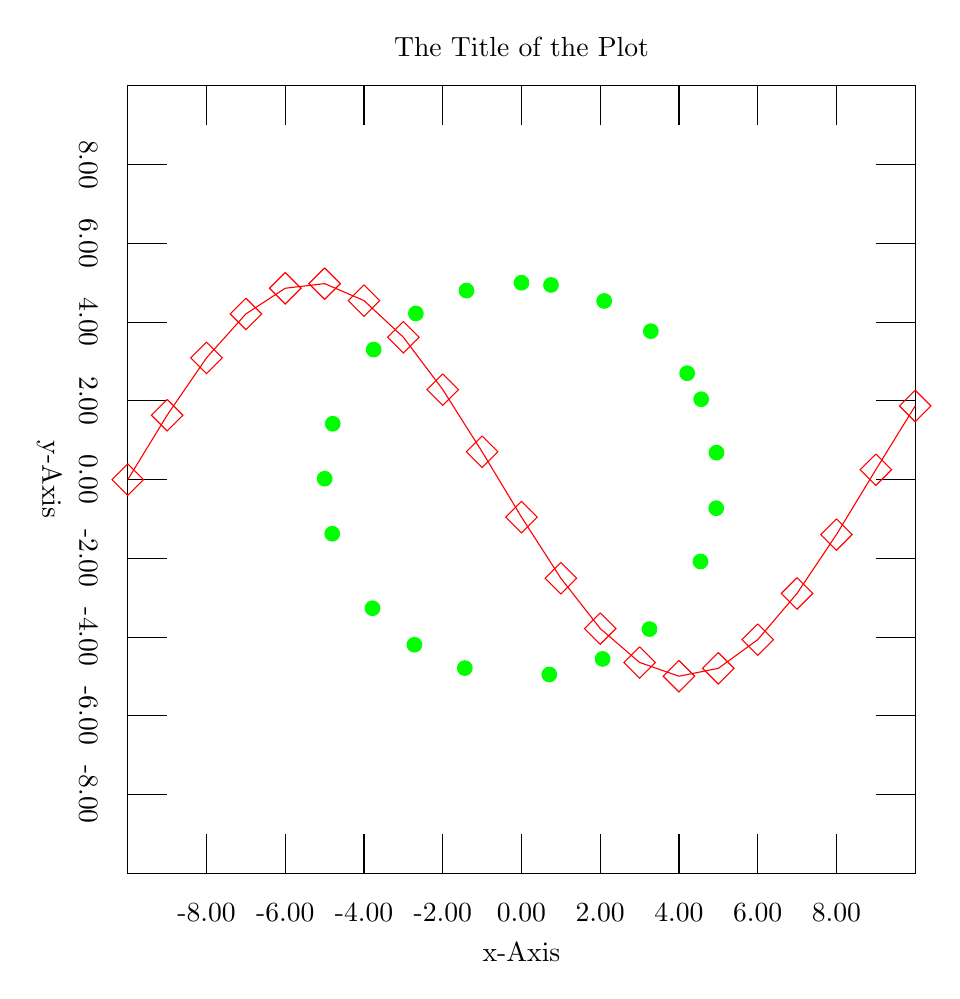
\begin{tikzpicture}
\draw ( 1.00000E+00, 1.00000E+00) rectangle ( 1.10000E+01, 1.10000E+01);
\draw ( 2.00000E+00, 1.00000E+00) -- ( 2.00000E+00, 1.50000E+00);
\draw ( 2.00000E+00, 1.05000E+01) -- ( 2.00000E+00, 1.10000E+01);
\node at ( 2.00000E+00, 5.00000E-01) {-8.00};
\draw ( 3.00000E+00, 1.00000E+00) -- ( 3.00000E+00, 1.50000E+00);
\draw ( 3.00000E+00, 1.05000E+01) -- ( 3.00000E+00, 1.10000E+01);
\node at ( 3.00000E+00, 5.00000E-01) {-6.00};
\draw ( 4.00000E+00, 1.00000E+00) -- ( 4.00000E+00, 1.50000E+00);
\draw ( 4.00000E+00, 1.05000E+01) -- ( 4.00000E+00, 1.10000E+01);
\node at ( 4.00000E+00, 5.00000E-01) {-4.00};
\draw ( 5.00000E+00, 1.00000E+00) -- ( 5.00000E+00, 1.50000E+00);
\draw ( 5.00000E+00, 1.05000E+01) -- ( 5.00000E+00, 1.10000E+01);
\node at ( 5.00000E+00, 5.00000E-01) {-2.00};
\draw ( 6.00000E+00, 1.00000E+00) -- ( 6.00000E+00, 1.50000E+00);
\draw ( 6.00000E+00, 1.05000E+01) -- ( 6.00000E+00, 1.10000E+01);
\node at ( 6.00000E+00, 5.00000E-01) { 0.00};
\draw ( 7.00000E+00, 1.00000E+00) -- ( 7.00000E+00, 1.50000E+00);
\draw ( 7.00000E+00, 1.05000E+01) -- ( 7.00000E+00, 1.10000E+01);
\node at ( 7.00000E+00, 5.00000E-01) { 2.00};
\draw ( 8.00000E+00, 1.00000E+00) -- ( 8.00000E+00, 1.50000E+00);
\draw ( 8.00000E+00, 1.05000E+01) -- ( 8.00000E+00, 1.10000E+01);
\node at ( 8.00000E+00, 5.00000E-01) { 4.00};
\draw ( 9.00000E+00, 1.00000E+00) -- ( 9.00000E+00, 1.50000E+00);
\draw ( 9.00000E+00, 1.05000E+01) -- ( 9.00000E+00, 1.10000E+01);
\node at ( 9.00000E+00, 5.00000E-01) { 6.00};
\draw ( 1.00000E+01, 1.00000E+00) -- ( 1.00000E+01, 1.50000E+00);
\draw ( 1.00000E+01, 1.05000E+01) -- ( 1.00000E+01, 1.10000E+01);
\node at ( 1.00000E+01, 5.00000E-01) { 8.00};
\draw ( 1.00000E+00, 2.00000E+00) -- ( 1.50000E+00, 2.00000E+00);\draw ( 1.05000E+01, 2.00000E+00) -- ( 1.10000E+01, 2.00000E+00);
\node [rotate=-90] at ( 5.00000E-01, 2.00000E+00) {-8.00};
\draw ( 1.00000E+00, 3.00000E+00) -- ( 1.50000E+00, 3.00000E+00);\draw ( 1.05000E+01, 3.00000E+00) -- ( 1.10000E+01, 3.00000E+00);
\node [rotate=-90] at ( 5.00000E-01, 3.00000E+00) {-6.00};
\draw ( 1.00000E+00, 4.00000E+00) -- ( 1.50000E+00, 4.00000E+00);\draw ( 1.05000E+01, 4.00000E+00) -- ( 1.10000E+01, 4.00000E+00);
\node [rotate=-90] at ( 5.00000E-01, 4.00000E+00) {-4.00};
\draw ( 1.00000E+00, 5.00000E+00) -- ( 1.50000E+00, 5.00000E+00);\draw ( 1.05000E+01, 5.00000E+00) -- ( 1.10000E+01, 5.00000E+00);
\node [rotate=-90] at ( 5.00000E-01, 5.00000E+00) {-2.00};
\draw ( 1.00000E+00, 6.00000E+00) -- ( 1.50000E+00, 6.00000E+00);\draw ( 1.05000E+01, 6.00000E+00) -- ( 1.10000E+01, 6.00000E+00);
\node [rotate=-90] at ( 5.00000E-01, 6.00000E+00) { 0.00};
\draw ( 1.00000E+00, 7.00000E+00) -- ( 1.50000E+00, 7.00000E+00);\draw ( 1.05000E+01, 7.00000E+00) -- ( 1.10000E+01, 7.00000E+00);
\node [rotate=-90] at ( 5.00000E-01, 7.00000E+00) { 2.00};
\draw ( 1.00000E+00, 8.00000E+00) -- ( 1.50000E+00, 8.00000E+00);\draw ( 1.05000E+01, 8.00000E+00) -- ( 1.10000E+01, 8.00000E+00);
\node [rotate=-90] at ( 5.00000E-01, 8.00000E+00) { 4.00};
\draw ( 1.00000E+00, 9.00000E+00) -- ( 1.50000E+00, 9.00000E+00);\draw ( 1.05000E+01, 9.00000E+00) -- ( 1.10000E+01, 9.00000E+00);
\node [rotate=-90] at ( 5.00000E-01, 9.00000E+00) { 6.00};
\draw ( 1.00000E+00, 1.00000E+01) -- ( 1.50000E+00, 1.00000E+01);\draw ( 1.05000E+01, 1.00000E+01) -- ( 1.10000E+01, 1.00000E+01);
\node [rotate=-90] at ( 5.00000E-01, 1.00000E+01) { 8.00};
\node at ( 6.00000E+00, 0.00000E+00) {x-Axis};
\node [rotate=-90] at ( 0.00000E+00, 6.00000E+00) {y-Axis};
\node at ( 6.00000E+00, 1.15000E+01) {The Title of the Plot};
\draw [red] ( 1.00000E+00, 6.00000E+00) -- ( 1.50000E+00, 6.81799E+00) -- ( 2.00000E+00, 7.54592E+00) -- ( 2.50000E+00, 8.10368E+00) -- ( 3.00000E+00, 8.42984E+00) -- ( 3.50000E+00, 8.48852E+00) -- ( 4.00000E+00, 8.27324E+00) -- ( 4.50000E+00, 7.80771E+00) -- ( 5.00000E+00, 7.14318E+00) -- ( 5.50000E+00, 6.35280E+00) -- ( 6.00000E+00, 5.52358E+00) -- ( 6.50000E+00, 4.74681E+00) -- ( 7.00000E+00, 4.10799E+00) -- ( 7.50000E+00, 3.67746E+00) -- ( 8.00000E+00, 3.50261E+00) -- ( 8.50000E+00, 3.60269E+00) -- ( 9.00000E+00, 3.96668E+00) -- ( 9.50000E+00, 4.55450E+00) -- ( 1.00000E+01, 5.30146E+00) -- ( 1.05000E+01, 6.12532E+00) -- ( 1.10000E+01, 6.93538E+00);
<g stroke="red" stroke-width="1">
\draw [red] ( 1.00000E+00, 6.20000E+00) -- ( 8.00000E-01, 6.00000E+00) -- ( 1.00000E+00, 5.80000E+00) -- ( 1.20000E+00, 6.00000E+00) -- ( 1.00000E+00, 6.20000E+00);
\draw [red] ( 1.50000E+00, 7.01799E+00) -- ( 1.30000E+00, 6.81799E+00) -- ( 1.50000E+00, 6.61799E+00) -- ( 1.70000E+00, 6.81799E+00) -- ( 1.50000E+00, 7.01799E+00);
\draw [red] ( 2.00000E+00, 7.74592E+00) -- ( 1.80000E+00, 7.54592E+00) -- ( 2.00000E+00, 7.34592E+00) -- ( 2.20000E+00, 7.54592E+00) -- ( 2.00000E+00, 7.74592E+00);
\draw [red] ( 2.50000E+00, 8.30368E+00) -- ( 2.30000E+00, 8.10368E+00) -- ( 2.50000E+00, 7.90368E+00) -- ( 2.70000E+00, 8.10368E+00) -- ( 2.50000E+00, 8.30368E+00);
\draw [red] ( 3.00000E+00, 8.62984E+00) -- ( 2.80000E+00, 8.42984E+00) -- ( 3.00000E+00, 8.22985E+00) -- ( 3.20000E+00, 8.42984E+00) -- ( 3.00000E+00, 8.62984E+00);
\draw [red] ( 3.50000E+00, 8.68852E+00) -- ( 3.30000E+00, 8.48852E+00) -- ( 3.50000E+00, 8.28852E+00) -- ( 3.70000E+00, 8.48852E+00) -- ( 3.50000E+00, 8.68852E+00);
\draw [red] ( 4.00000E+00, 8.47324E+00) -- ( 3.80000E+00, 8.27324E+00) -- ( 4.00000E+00, 8.07324E+00) -- ( 4.20000E+00, 8.27324E+00) -- ( 4.00000E+00, 8.47324E+00);
\draw [red] ( 4.50000E+00, 8.00772E+00) -- ( 4.30000E+00, 7.80771E+00) -- ( 4.50000E+00, 7.60772E+00) -- ( 4.70000E+00, 7.80771E+00) -- ( 4.50000E+00, 8.00772E+00);
\draw [red] ( 5.00000E+00, 7.34318E+00) -- ( 4.80000E+00, 7.14318E+00) -- ( 5.00000E+00, 6.94318E+00) -- ( 5.20000E+00, 7.14318E+00) -- ( 5.00000E+00, 7.34318E+00);
\draw [red] ( 5.50000E+00, 6.55280E+00) -- ( 5.30000E+00, 6.35280E+00) -- ( 5.50000E+00, 6.15280E+00) -- ( 5.70000E+00, 6.35280E+00) -- ( 5.50000E+00, 6.55280E+00);
\draw [red] ( 6.00000E+00, 5.72358E+00) -- ( 5.80000E+00, 5.52358E+00) -- ( 6.00000E+00, 5.32358E+00) -- ( 6.20000E+00, 5.52358E+00) -- ( 6.00000E+00, 5.72358E+00);
\draw [red] ( 6.50000E+00, 4.94681E+00) -- ( 6.30000E+00, 4.74681E+00) -- ( 6.50000E+00, 4.54681E+00) -- ( 6.70000E+00, 4.74681E+00) -- ( 6.50000E+00, 4.94681E+00);
\draw [red] ( 7.00000E+00, 4.30799E+00) -- ( 6.80000E+00, 4.10799E+00) -- ( 7.00000E+00, 3.90799E+00) -- ( 7.20000E+00, 4.10799E+00) -- ( 7.00000E+00, 4.30799E+00);
\draw [red] ( 7.50000E+00, 3.87746E+00) -- ( 7.30000E+00, 3.67746E+00) -- ( 7.50000E+00, 3.47746E+00) -- ( 7.70000E+00, 3.67746E+00) -- ( 7.50000E+00, 3.87746E+00);
\draw [red] ( 8.00000E+00, 3.70261E+00) -- ( 7.80000E+00, 3.50261E+00) -- ( 8.00000E+00, 3.30261E+00) -- ( 8.20000E+00, 3.50261E+00) -- ( 8.00000E+00, 3.70261E+00);
\draw [red] ( 8.50000E+00, 3.80269E+00) -- ( 8.30000E+00, 3.60269E+00) -- ( 8.50000E+00, 3.40269E+00) -- ( 8.70000E+00, 3.60269E+00) -- ( 8.50000E+00, 3.80269E+00);
\draw [red] ( 9.00000E+00, 4.16668E+00) -- ( 8.80000E+00, 3.96668E+00) -- ( 9.00000E+00, 3.76668E+00) -- ( 9.20000E+00, 3.96668E+00) -- ( 9.00000E+00, 4.16668E+00);
\draw [red] ( 9.50000E+00, 4.75450E+00) -- ( 9.30000E+00, 4.55450E+00) -- ( 9.50000E+00, 4.35450E+00) -- ( 9.70000E+00, 4.55450E+00) -- ( 9.50000E+00, 4.75450E+00);
\draw [red] ( 1.00000E+01, 5.50146E+00) -- ( 9.80000E+00, 5.30146E+00) -- ( 1.00000E+01, 5.10146E+00) -- ( 1.02000E+01, 5.30146E+00) -- ( 1.00000E+01, 5.50146E+00);
\draw [red] ( 1.05000E+01, 6.32532E+00) -- ( 1.03000E+01, 6.12532E+00) -- ( 1.05000E+01, 5.92532E+00) -- ( 1.07000E+01, 6.12532E+00) -- ( 1.05000E+01, 6.32532E+00);
\draw [red] ( 1.10000E+01, 7.13538E+00) -- ( 1.08000E+01, 6.93538E+00) -- ( 1.10000E+01, 6.73538E+00) -- ( 1.12000E+01, 6.93538E+00) -- ( 1.10000E+01, 7.13538E+00);
</g>
\path [fill=green] ( 6.00000E+00, 8.50000E+00) circle [radius= 1.00000E-01];
\path [fill=green] ( 8.10368E+00, 7.35076E+00) circle [radius= 1.00000E-01];
\path [fill=green] ( 8.27324E+00, 4.95963E+00) circle [radius= 1.00000E-01];
\path [fill=green] ( 6.35280E+00, 3.52502E+00) circle [radius= 1.00000E-01];
\path [fill=green] ( 4.10799E+00, 4.36589E+00) circle [radius= 1.00000E-01];
\path [fill=green] ( 3.60269E+00, 6.70916E+00) circle [radius= 1.00000E-01];
\path [fill=green] ( 5.30146E+00, 8.40043E+00) circle [radius= 1.00000E-01];
\path [fill=green] ( 7.64247E+00, 7.88476E+00) circle [radius= 1.00000E-01];
\path [fill=green] ( 8.47340E+00, 5.63625E+00) circle [radius= 1.00000E-01];
\path [fill=green] ( 7.03030E+00, 3.72217E+00) circle [radius= 1.00000E-01];
\path [fill=green] ( 4.63995E+00, 3.90232E+00) circle [radius= 1.00000E-01];
\path [fill=green] ( 3.50002E+00, 6.01106E+00) circle [radius= 1.00000E-01];
\path [fill=green] ( 4.65857E+00, 8.10964E+00) circle [radius= 1.00000E-01];
\path [fill=green] ( 7.05042E+00, 8.26862E+00) circle [radius= 1.00000E-01];
\path [fill=green] ( 8.47652E+00, 6.34184E+00) circle [radius= 1.00000E-01];
\path [fill=green] ( 7.62572E+00, 4.10078E+00) circle [radius= 1.00000E-01];
\path [fill=green] ( 5.28024E+00, 3.60585E+00) circle [radius= 1.00000E-01];
\path [fill=green] ( 3.59651E+00, 5.31209E+00) circle [radius= 1.00000E-01];
\path [fill=green] ( 4.12253E+00, 7.65079E+00) circle [radius= 1.00000E-01];
\path [fill=green] ( 6.37469E+00, 8.47176E+00) circle [radius= 1.00000E-01];
\path [fill=green] ( 8.28236E+00, 7.02021E+00) circle [radius= 1.00000E-01];
\end{tikzpicture}

  \caption{A Sample Figure}
\end{figure}
\end{lstlisting}

Some example figures are shown in Figures \ref{tex:Ave} and \ref{tex:Prob}.

\begin{figure}
  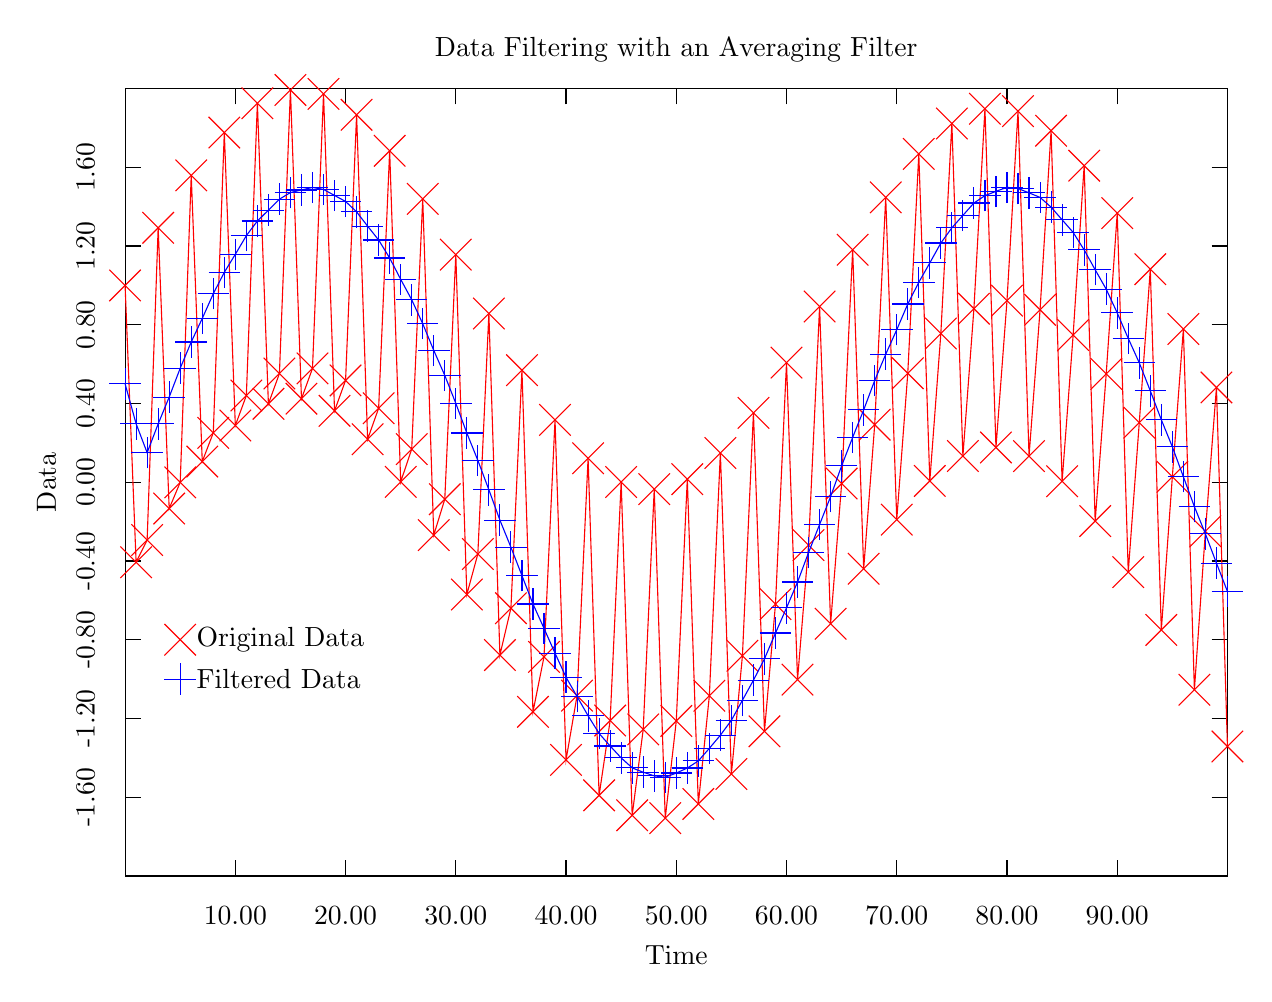
\begin{tikzpicture}
\draw ( 1.00000E+00, 1.00000E+00) rectangle ( 1.50000E+01, 1.10000E+01);
\draw ( 2.40000E+00, 1.00000E+00) -- ( 2.40000E+00, 1.20000E+00);
\draw ( 2.40000E+00, 1.08000E+01) -- ( 2.40000E+00, 1.10000E+01);
\node at ( 2.40000E+00, 5.00000E-01) {10.00};
\draw ( 3.80000E+00, 1.00000E+00) -- ( 3.80000E+00, 1.20000E+00);
\draw ( 3.80000E+00, 1.08000E+01) -- ( 3.80000E+00, 1.10000E+01);
\node at ( 3.80000E+00, 5.00000E-01) {20.00};
\draw ( 5.20000E+00, 1.00000E+00) -- ( 5.20000E+00, 1.20000E+00);
\draw ( 5.20000E+00, 1.08000E+01) -- ( 5.20000E+00, 1.10000E+01);
\node at ( 5.20000E+00, 5.00000E-01) {30.00};
\draw ( 6.60000E+00, 1.00000E+00) -- ( 6.60000E+00, 1.20000E+00);
\draw ( 6.60000E+00, 1.08000E+01) -- ( 6.60000E+00, 1.10000E+01);
\node at ( 6.60000E+00, 5.00000E-01) {40.00};
\draw ( 8.00000E+00, 1.00000E+00) -- ( 8.00000E+00, 1.20000E+00);
\draw ( 8.00000E+00, 1.08000E+01) -- ( 8.00000E+00, 1.10000E+01);
\node at ( 8.00000E+00, 5.00000E-01) {50.00};
\draw ( 9.40000E+00, 1.00000E+00) -- ( 9.40000E+00, 1.20000E+00);
\draw ( 9.40000E+00, 1.08000E+01) -- ( 9.40000E+00, 1.10000E+01);
\node at ( 9.40000E+00, 5.00000E-01) {60.00};
\draw ( 1.08000E+01, 1.00000E+00) -- ( 1.08000E+01, 1.20000E+00);
\draw ( 1.08000E+01, 1.08000E+01) -- ( 1.08000E+01, 1.10000E+01);
\node at ( 1.08000E+01, 5.00000E-01) {70.00};
\draw ( 1.22000E+01, 1.00000E+00) -- ( 1.22000E+01, 1.20000E+00);
\draw ( 1.22000E+01, 1.08000E+01) -- ( 1.22000E+01, 1.10000E+01);
\node at ( 1.22000E+01, 5.00000E-01) {80.00};
\draw ( 1.36000E+01, 1.00000E+00) -- ( 1.36000E+01, 1.20000E+00);
\draw ( 1.36000E+01, 1.08000E+01) -- ( 1.36000E+01, 1.10000E+01);
\node at ( 1.36000E+01, 5.00000E-01) {90.00};
\draw ( 1.00000E+00, 2.00000E+00) -- ( 1.20000E+00, 2.00000E+00);\draw ( 1.48000E+01, 2.00000E+00) -- ( 1.50000E+01, 2.00000E+00);
\node [rotate=90] at ( 5.00000E-01, 2.00000E+00) {-1.60};
\draw ( 1.00000E+00, 3.00000E+00) -- ( 1.20000E+00, 3.00000E+00);\draw ( 1.48000E+01, 3.00000E+00) -- ( 1.50000E+01, 3.00000E+00);
\node [rotate=90] at ( 5.00000E-01, 3.00000E+00) {-1.20};
\draw ( 1.00000E+00, 4.00000E+00) -- ( 1.20000E+00, 4.00000E+00);\draw ( 1.48000E+01, 4.00000E+00) -- ( 1.50000E+01, 4.00000E+00);
\node [rotate=90] at ( 5.00000E-01, 4.00000E+00) {-0.80};
\draw ( 1.00000E+00, 5.00000E+00) -- ( 1.20000E+00, 5.00000E+00);\draw ( 1.48000E+01, 5.00000E+00) -- ( 1.50000E+01, 5.00000E+00);
\node [rotate=90] at ( 5.00000E-01, 5.00000E+00) {-0.40};
\draw ( 1.00000E+00, 6.00000E+00) -- ( 1.20000E+00, 6.00000E+00);\draw ( 1.48000E+01, 6.00000E+00) -- ( 1.50000E+01, 6.00000E+00);
\node [rotate=90] at ( 5.00000E-01, 6.00000E+00) { 0.00};
\draw ( 1.00000E+00, 7.00000E+00) -- ( 1.20000E+00, 7.00000E+00);\draw ( 1.48000E+01, 7.00000E+00) -- ( 1.50000E+01, 7.00000E+00);
\node [rotate=90] at ( 5.00000E-01, 7.00000E+00) { 0.40};
\draw ( 1.00000E+00, 8.00000E+00) -- ( 1.20000E+00, 8.00000E+00);\draw ( 1.48000E+01, 8.00000E+00) -- ( 1.50000E+01, 8.00000E+00);
\node [rotate=90] at ( 5.00000E-01, 8.00000E+00) { 0.80};
\draw ( 1.00000E+00, 9.00000E+00) -- ( 1.20000E+00, 9.00000E+00);\draw ( 1.48000E+01, 9.00000E+00) -- ( 1.50000E+01, 9.00000E+00);
\node [rotate=90] at ( 5.00000E-01, 9.00000E+00) { 1.20};
\draw ( 1.00000E+00, 1.00000E+01) -- ( 1.20000E+00, 1.00000E+01);\draw ( 1.48000E+01, 1.00000E+01) -- ( 1.50000E+01, 1.00000E+01);
\node [rotate=90] at ( 5.00000E-01, 1.00000E+01) { 1.60};
\node at ( 8.00000E+00, 0.00000E+00) {Time};
\node [rotate=90] at ( 0.00000E+00, 6.00000E+00) {Data};
\node at ( 8.00000E+00, 1.15000E+01) {Data Filtering with an Averaging Filter};
\draw [red] ( 8.00000E-01, 8.30000E+00) -- ( 1.20000E+00, 8.70000E+00);
\draw [red] ( 1.20000E+00, 8.30000E+00) -- ( 8.00000E-01, 8.70000E+00);
\draw [red] ( 9.40000E-01, 4.78501E+00) -- ( 1.34000E+00, 5.18501E+00);
\draw [red] ( 1.34000E+00, 4.78501E+00) -- ( 9.40000E-01, 5.18501E+00);
\draw [red] ( 1.08000E+00, 5.06617E+00) -- ( 1.48000E+00, 5.46617E+00);
\draw [red] ( 1.48000E+00, 5.06617E+00) -- ( 1.08000E+00, 5.46617E+00);
\draw [red] ( 1.22000E+00, 9.03135E+00) -- ( 1.62000E+00, 9.43135E+00);
\draw [red] ( 1.62000E+00, 9.03135E+00) -- ( 1.22000E+00, 9.43135E+00);
\draw [red] ( 1.36000E+00, 5.46620E+00) -- ( 1.76000E+00, 5.86620E+00);
\draw [red] ( 1.76000E+00, 5.46620E+00) -- ( 1.36000E+00, 5.86620E+00);
\draw [red] ( 1.50000E+00, 5.79885E+00) -- ( 1.90000E+00, 6.19885E+00);
\draw [red] ( 1.90000E+00, 5.79885E+00) -- ( 1.50000E+00, 6.19885E+00);
\draw [red] ( 1.64000E+00, 9.69791E+00) -- ( 2.04000E+00, 1.00979E+01);
\draw [red] ( 2.04000E+00, 9.69791E+00) -- ( 1.64000E+00, 1.00979E+01);
\draw [red] ( 1.78000E+00, 6.06330E+00) -- ( 2.18000E+00, 6.46329E+00);
\draw [red] ( 2.18000E+00, 6.06330E+00) -- ( 1.78000E+00, 6.46329E+00);
\draw [red] ( 1.92000E+00, 6.42784E+00) -- ( 2.32000E+00, 6.82784E+00);
\draw [red] ( 2.32000E+00, 6.42784E+00) -- ( 1.92000E+00, 6.82784E+00);
\draw [red] ( 2.06000E+00, 1.02412E+01) -- ( 2.46000E+00, 1.06412E+01);
\draw [red] ( 2.46000E+00, 1.02412E+01) -- ( 2.06000E+00, 1.06412E+01);
\draw [red] ( 2.20000E+00, 6.52088E+00) -- ( 2.60000E+00, 6.92088E+00);
\draw [red] ( 2.60000E+00, 6.52088E+00) -- ( 2.20000E+00, 6.92088E+00);
\draw [red] ( 2.34000E+00, 6.90131E+00) -- ( 2.74000E+00, 7.30131E+00);
\draw [red] ( 2.74000E+00, 6.90131E+00) -- ( 2.34000E+00, 7.30131E+00);
\draw [red] ( 2.48000E+00, 1.06135E+01) -- ( 2.88000E+00, 1.10135E+01);
\draw [red] ( 2.88000E+00, 1.06135E+01) -- ( 2.48000E+00, 1.10135E+01);
\draw [red] ( 2.62000E+00, 6.79579E+00) -- ( 3.02000E+00, 7.19579E+00);
\draw [red] ( 3.02000E+00, 6.79579E+00) -- ( 2.62000E+00, 7.19579E+00);
\draw [red] ( 2.76000E+00, 7.18105E+00) -- ( 3.16000E+00, 7.58105E+00);
\draw [red] ( 3.16000E+00, 7.18105E+00) -- ( 2.76000E+00, 7.58105E+00);
\draw [red] ( 2.90000E+00, 1.07820E+01) -- ( 3.30000E+00, 1.11820E+01);
\draw [red] ( 3.30000E+00, 1.07820E+01) -- ( 2.90000E+00, 1.11820E+01);
\draw [red] ( 3.04000E+00, 6.86090E+00) -- ( 3.44000E+00, 7.26090E+00);
\draw [red] ( 3.44000E+00, 6.86090E+00) -- ( 3.04000E+00, 7.26090E+00);
\draw [red] ( 3.18000E+00, 7.24588E+00) -- ( 3.58000E+00, 7.64588E+00);
\draw [red] ( 3.58000E+00, 7.24588E+00) -- ( 3.18000E+00, 7.64588E+00);
\draw [red] ( 3.32000E+00, 1.07316E+01) -- ( 3.72000E+00, 1.11316E+01);
\draw [red] ( 3.72000E+00, 1.07316E+01) -- ( 3.32000E+00, 1.11316E+01);
\draw [red] ( 3.46000E+00, 6.70749E+00) -- ( 3.86000E+00, 7.10749E+00);
\draw [red] ( 3.86000E+00, 6.70749E+00) -- ( 3.46000E+00, 7.10749E+00);
\draw [red] ( 3.60000E+00, 7.09343E+00) -- ( 4.00000E+00, 7.49343E+00);
\draw [red] ( 4.00000E+00, 7.09343E+00) -- ( 3.60000E+00, 7.49343E+00);
\draw [red] ( 3.74000E+00, 1.04665E+01) -- ( 4.14000E+00, 1.08665E+01);
\draw [red] ( 4.14000E+00, 1.04665E+01) -- ( 3.74000E+00, 1.08665E+01);
\draw [red] ( 3.88000E+00, 6.34601E+00) -- ( 4.28000E+00, 6.74601E+00);
\draw [red] ( 4.28000E+00, 6.34601E+00) -- ( 3.88000E+00, 6.74601E+00);
\draw [red] ( 4.02000E+00, 6.74041E+00) -- ( 4.42000E+00, 7.14041E+00);
\draw [red] ( 4.42000E+00, 6.74041E+00) -- ( 4.02000E+00, 7.14041E+00);
\draw [red] ( 4.16000E+00, 1.00094E+01) -- ( 4.56000E+00, 1.04094E+01);
\draw [red] ( 4.56000E+00, 1.00094E+01) -- ( 4.16000E+00, 1.04094E+01);
\draw [red] ( 4.30000E+00, 5.80517E+00) -- ( 4.70000E+00, 6.20517E+00);
\draw [red] ( 4.70000E+00, 5.80517E+00) -- ( 4.30000E+00, 6.20517E+00);
\draw [red] ( 4.44000E+00, 6.22111E+00) -- ( 4.84000E+00, 6.62111E+00);
\draw [red] ( 4.84000E+00, 6.22111E+00) -- ( 4.44000E+00, 6.62111E+00);
\draw [red] ( 4.58000E+00, 9.39991E+00) -- ( 4.98000E+00, 9.79991E+00);
\draw [red] ( 4.98000E+00, 9.39991E+00) -- ( 4.58000E+00, 9.79991E+00);
\draw [red] ( 4.72000E+00, 5.12943E+00) -- ( 5.12000E+00, 5.52943E+00);
\draw [red] ( 5.12000E+00, 5.12943E+00) -- ( 4.72000E+00, 5.52943E+00);
\draw [red] ( 4.86000E+00, 5.58440E+00) -- ( 5.26000E+00, 5.98440E+00);
\draw [red] ( 5.26000E+00, 5.58440E+00) -- ( 4.86000E+00, 5.98440E+00);
\draw [red] ( 5.00000E+00, 8.69089E+00) -- ( 5.40000E+00, 9.09089E+00);
\draw [red] ( 5.40000E+00, 8.69089E+00) -- ( 5.00000E+00, 9.09089E+00);
\draw [red] ( 5.14000E+00, 4.37509E+00) -- ( 5.54000E+00, 4.77509E+00);
\draw [red] ( 5.54000E+00, 4.37509E+00) -- ( 5.14000E+00, 4.77509E+00);
\draw [red] ( 5.28000E+00, 4.88948E+00) -- ( 5.68000E+00, 5.28948E+00);
\draw [red] ( 5.68000E+00, 4.88948E+00) -- ( 5.28000E+00, 5.28948E+00);
\draw [red] ( 5.42000E+00, 7.94385E+00) -- ( 5.82000E+00, 8.34385E+00);
\draw [red] ( 5.82000E+00, 7.94385E+00) -- ( 5.42000E+00, 8.34385E+00);
\draw [red] ( 5.56000E+00, 3.60540E+00) -- ( 5.96000E+00, 4.00540E+00);
\draw [red] ( 5.96000E+00, 3.60540E+00) -- ( 5.56000E+00, 4.00540E+00);
\draw [red] ( 5.70000E+00, 4.20066E+00) -- ( 6.10000E+00, 4.60066E+00);
\draw [red] ( 6.10000E+00, 4.20066E+00) -- ( 5.70000E+00, 4.60066E+00);
\draw [red] ( 5.84000E+00, 7.22358E+00) -- ( 6.24000E+00, 7.62358E+00);
\draw [red] ( 6.24000E+00, 7.22358E+00) -- ( 5.84000E+00, 7.62358E+00);
\draw [red] ( 5.98000E+00, 2.88496E+00) -- ( 6.38000E+00, 3.28496E+00);
\draw [red] ( 6.38000E+00, 2.88496E+00) -- ( 5.98000E+00, 3.28496E+00);
\draw [red] ( 6.12000E+00, 3.58170E+00) -- ( 6.52000E+00, 3.98170E+00);
\draw [red] ( 6.52000E+00, 3.58170E+00) -- ( 6.12000E+00, 3.98170E+00);
\draw [red] ( 6.26000E+00, 6.59244E+00) -- ( 6.66000E+00, 6.99244E+00);
\draw [red] ( 6.66000E+00, 6.59244E+00) -- ( 6.26000E+00, 6.99244E+00);
\draw [red] ( 6.40000E+00, 2.27412E+00) -- ( 6.80000E+00, 2.67412E+00);
\draw [red] ( 6.80000E+00, 2.27412E+00) -- ( 6.40000E+00, 2.67412E+00);
\draw [red] ( 6.54000E+00, 3.09034E+00) -- ( 6.94000E+00, 3.49034E+00);
\draw [red] ( 6.94000E+00, 3.09034E+00) -- ( 6.54000E+00, 3.49034E+00);
\draw [red] ( 6.68000E+00, 6.10495E+00) -- ( 7.08000E+00, 6.50495E+00);
\draw [red] ( 7.08000E+00, 6.10495E+00) -- ( 6.68000E+00, 6.50495E+00);
\draw [red] ( 6.82000E+00, 1.82368E+00) -- ( 7.22000E+00, 2.22368E+00);
\draw [red] ( 7.22000E+00, 1.82368E+00) -- ( 6.82000E+00, 2.22368E+00);
\draw [red] ( 6.96000E+00, 2.77306E+00) -- ( 7.36000E+00, 3.17306E+00);
\draw [red] ( 7.36000E+00, 2.77306E+00) -- ( 6.96000E+00, 3.17306E+00);
\draw [red] ( 7.10000E+00, 5.80298E+00) -- ( 7.50000E+00, 6.20298E+00);
\draw [red] ( 7.50000E+00, 5.80298E+00) -- ( 7.10000E+00, 6.20298E+00);
\draw [red] ( 7.24000E+00, 1.57039E+00) -- ( 7.64000E+00, 1.97039E+00);
\draw [red] ( 7.64000E+00, 1.57039E+00) -- ( 7.24000E+00, 1.97039E+00);
\draw [red] ( 7.38000E+00, 2.66122E+00) -- ( 7.78000E+00, 3.06122E+00);
\draw [red] ( 7.78000E+00, 2.66122E+00) -- ( 7.38000E+00, 3.06122E+00);
\draw [red] ( 7.52000E+00, 5.71208E+00) -- ( 7.92000E+00, 6.11208E+00);
\draw [red] ( 7.92000E+00, 5.71208E+00) -- ( 7.52000E+00, 6.11208E+00);
\draw [red] ( 7.66000E+00, 1.53384E+00) -- ( 8.06000E+00, 1.93384E+00);
\draw [red] ( 8.06000E+00, 1.53384E+00) -- ( 7.66000E+00, 1.93384E+00);
\draw [red] ( 7.80000E+00, 2.76812E+00) -- ( 8.20000E+00, 3.16812E+00);
\draw [red] ( 8.20000E+00, 2.76812E+00) -- ( 7.80000E+00, 3.16812E+00);
\draw [red] ( 7.94000E+00, 5.83928E+00) -- ( 8.34000E+00, 6.23928E+00);
\draw [red] ( 8.34000E+00, 5.83928E+00) -- ( 7.94000E+00, 6.23928E+00);
\draw [red] ( 8.08000E+00, 1.71461E+00) -- ( 8.48000E+00, 2.11461E+00);
\draw [red] ( 8.48000E+00, 1.71461E+00) -- ( 8.08000E+00, 2.11461E+00);
\draw [red] ( 8.22000E+00, 3.08797E+00) -- ( 8.62000E+00, 3.48797E+00);
\draw [red] ( 8.62000E+00, 3.08797E+00) -- ( 8.22000E+00, 3.48797E+00);
\draw [red] ( 8.36000E+00, 6.17242E+00) -- ( 8.76000E+00, 6.57242E+00);
\draw [red] ( 8.76000E+00, 6.17242E+00) -- ( 8.36000E+00, 6.57242E+00);
\draw [red] ( 8.50000E+00, 2.09437E+00) -- ( 8.90000E+00, 2.49437E+00);
\draw [red] ( 8.90000E+00, 2.09437E+00) -- ( 8.50000E+00, 2.49437E+00);
\draw [red] ( 8.64000E+00, 3.59631E+00) -- ( 9.04000E+00, 3.99631E+00);
\draw [red] ( 9.04000E+00, 3.59631E+00) -- ( 8.64000E+00, 3.99631E+00);
\draw [red] ( 8.78000E+00, 6.68127E+00) -- ( 9.18000E+00, 7.08127E+00);
\draw [red] ( 9.18000E+00, 6.68127E+00) -- ( 8.78000E+00, 7.08127E+00);
\draw [red] ( 8.92000E+00, 2.63733E+00) -- ( 9.32000E+00, 3.03733E+00);
\draw [red] ( 9.32000E+00, 2.63733E+00) -- ( 8.92000E+00, 3.03733E+00);
\draw [red] ( 9.06000E+00, 4.25223E+00) -- ( 9.46000E+00, 4.65223E+00);
\draw [red] ( 9.46000E+00, 4.25223E+00) -- ( 9.06000E+00, 4.65223E+00);
\draw [red] ( 9.20000E+00, 7.32014E+00) -- ( 9.60000E+00, 7.72014E+00);
\draw [red] ( 9.60000E+00, 7.32014E+00) -- ( 9.20000E+00, 7.72014E+00);
\draw [red] ( 9.34000E+00, 3.29352E+00) -- ( 9.74000E+00, 3.69352E+00);
\draw [red] ( 9.74000E+00, 3.29352E+00) -- ( 9.34000E+00, 3.69352E+00);
\draw [red] ( 9.48000E+00, 5.00186E+00) -- ( 9.88000E+00, 5.40185E+00);
\draw [red] ( 9.88000E+00, 5.00186E+00) -- ( 9.48000E+00, 5.40185E+00);
\draw [red] ( 9.62000E+00, 8.03190E+00) -- ( 1.00200E+01, 8.43190E+00);
\draw [red] ( 1.00200E+01, 8.03190E+00) -- ( 9.62000E+00, 8.43190E+00);
\draw [red] ( 9.76000E+00, 4.00304E+00) -- ( 1.01600E+01, 4.40304E+00);
\draw [red] ( 1.01600E+01, 4.00304E+00) -- ( 9.76000E+00, 4.40304E+00);
\draw [red] ( 9.90000E+00, 5.78315E+00) -- ( 1.03000E+01, 6.18315E+00);
\draw [red] ( 1.03000E+01, 5.78315E+00) -- ( 9.90000E+00, 6.18315E+00);
\draw [red] ( 1.00400E+01, 8.75296E+00) -- ( 1.04400E+01, 9.15296E+00);
\draw [red] ( 1.04400E+01, 8.75296E+00) -- ( 1.00400E+01, 9.15296E+00);
\draw [red] ( 1.01800E+01, 4.70141E+00) -- ( 1.05800E+01, 5.10141E+00);
\draw [red] ( 1.05800E+01, 4.70141E+00) -- ( 1.01800E+01, 5.10141E+00);
\draw [red] ( 1.03200E+01, 6.53127E+00) -- ( 1.07200E+01, 6.93127E+00);
\draw [red] ( 1.07200E+01, 6.53127E+00) -- ( 1.03200E+01, 6.93127E+00);
\draw [red] ( 1.04600E+01, 9.41888E+00) -- ( 1.08600E+01, 9.81888E+00);
\draw [red] ( 1.08600E+01, 9.41888E+00) -- ( 1.04600E+01, 9.81888E+00);
\draw [red] ( 1.06000E+01, 5.32516E+00) -- ( 1.10000E+01, 5.72516E+00);
\draw [red] ( 1.10000E+01, 5.32516E+00) -- ( 1.06000E+01, 5.72516E+00);
\draw [red] ( 1.07400E+01, 7.18439E+00) -- ( 1.11400E+01, 7.58439E+00);
\draw [red] ( 1.11400E+01, 7.18439E+00) -- ( 1.07400E+01, 7.58439E+00);
\draw [red] ( 1.08800E+01, 9.96999E+00) -- ( 1.12800E+01, 1.03700E+01);
\draw [red] ( 1.12800E+01, 9.96999E+00) -- ( 1.08800E+01, 1.03700E+01);
\draw [red] ( 1.10200E+01, 5.81742E+00) -- ( 1.14200E+01, 6.21742E+00);
\draw [red] ( 1.14200E+01, 5.81742E+00) -- ( 1.10200E+01, 6.21742E+00);
\draw [red] ( 1.11600E+01, 7.68892E+00) -- ( 1.15600E+01, 8.08892E+00);
\draw [red] ( 1.15600E+01, 7.68892E+00) -- ( 1.11600E+01, 8.08892E+00);
\draw [red] ( 1.13000E+01, 1.03566E+01) -- ( 1.17000E+01, 1.07566E+01);
\draw [red] ( 1.17000E+01, 1.03566E+01) -- ( 1.13000E+01, 1.07566E+01);
\draw [red] ( 1.14400E+01, 6.13283E+00) -- ( 1.18400E+01, 6.53283E+00);
\draw [red] ( 1.18400E+01, 6.13283E+00) -- ( 1.14400E+01, 6.53283E+00);
\draw [red] ( 1.15800E+01, 8.00430E+00) -- ( 1.19800E+01, 8.40430E+00);
\draw [red] ( 1.19800E+01, 8.00430E+00) -- ( 1.15800E+01, 8.40430E+00);
\draw [red] ( 1.17200E+01, 1.05434E+01) -- ( 1.21200E+01, 1.09434E+01);
\draw [red] ( 1.21200E+01, 1.05434E+01) -- ( 1.17200E+01, 1.09434E+01);
\draw [red] ( 1.18600E+01, 6.24162E+00) -- ( 1.22600E+01, 6.64162E+00);
\draw [red] ( 1.22600E+01, 6.24162E+00) -- ( 1.18600E+01, 6.64162E+00);
\draw [red] ( 1.20000E+01, 8.10658E+00) -- ( 1.24000E+01, 8.50658E+00);
\draw [red] ( 1.24000E+01, 8.10658E+00) -- ( 1.20000E+01, 8.50658E+00);
\draw [red] ( 1.21400E+01, 1.05125E+01) -- ( 1.25400E+01, 1.09125E+01);
\draw [red] ( 1.25400E+01, 1.05125E+01) -- ( 1.21400E+01, 1.09125E+01);
\draw [red] ( 1.22800E+01, 6.13216E+00) -- ( 1.26800E+01, 6.53216E+00);
\draw [red] ( 1.26800E+01, 6.13216E+00) -- ( 1.22800E+01, 6.53216E+00);
\draw [red] ( 1.24200E+01, 7.99042E+00) -- ( 1.28200E+01, 8.39042E+00);
\draw [red] ( 1.28200E+01, 7.99042E+00) -- ( 1.24200E+01, 8.39042E+00);
\draw [red] ( 1.25600E+01, 1.02650E+01) -- ( 1.29600E+01, 1.06650E+01);
\draw [red] ( 1.29600E+01, 1.02650E+01) -- ( 1.25600E+01, 1.06650E+01);
\draw [red] ( 1.27000E+01, 5.81199E+00) -- ( 1.31000E+01, 6.21199E+00);
\draw [red] ( 1.31000E+01, 5.81199E+00) -- ( 1.27000E+01, 6.21199E+00);
\draw [red] ( 1.28400E+01, 7.66971E+00) -- ( 1.32400E+01, 8.06971E+00);
\draw [red] ( 1.32400E+01, 7.66971E+00) -- ( 1.28400E+01, 8.06971E+00);
\draw [red] ( 1.29800E+01, 9.82092E+00) -- ( 1.33800E+01, 1.02209E+01);
\draw [red] ( 1.33800E+01, 9.82092E+00) -- ( 1.29800E+01, 1.02209E+01);
\draw [red] ( 1.31200E+01, 5.30710E+00) -- ( 1.35200E+01, 5.70710E+00);
\draw [red] ( 1.35200E+01, 5.30710E+00) -- ( 1.31200E+01, 5.70710E+00);
\draw [red] ( 1.32600E+01, 7.17618E+00) -- ( 1.36600E+01, 7.57618E+00);
\draw [red] ( 1.36600E+01, 7.17618E+00) -- ( 1.32600E+01, 7.57618E+00);
\draw [red] ( 1.34000E+01, 9.21755E+00) -- ( 1.38000E+01, 9.61755E+00);
\draw [red] ( 1.38000E+01, 9.21755E+00) -- ( 1.34000E+01, 9.61755E+00);
\draw [red] ( 1.35400E+01, 4.65978E+00) -- ( 1.39400E+01, 5.05978E+00);
\draw [red] ( 1.39400E+01, 4.65978E+00) -- ( 1.35400E+01, 5.05978E+00);
\draw [red] ( 1.36800E+01, 6.55673E+00) -- ( 1.40800E+01, 6.95673E+00);
\draw [red] ( 1.40800E+01, 6.55673E+00) -- ( 1.36800E+01, 6.95673E+00);
\draw [red] ( 1.38200E+01, 8.50591E+00) -- ( 1.42200E+01, 8.90591E+00);
\draw [red] ( 1.42200E+01, 8.50591E+00) -- ( 1.38200E+01, 8.90591E+00);
\draw [red] ( 1.39600E+01, 3.92482E+00) -- ( 1.43600E+01, 4.32482E+00);
\draw [red] ( 1.43600E+01, 3.92482E+00) -- ( 1.39600E+01, 4.32482E+00);
\draw [red] ( 1.41000E+01, 5.86922E+00) -- ( 1.45000E+01, 6.26922E+00);
\draw [red] ( 1.45000E+01, 5.86922E+00) -- ( 1.41000E+01, 6.26922E+00);
\draw [red] ( 1.42400E+01, 7.74654E+00) -- ( 1.46400E+01, 8.14654E+00);
\draw [red] ( 1.46400E+01, 7.74654E+00) -- ( 1.42400E+01, 8.14654E+00);
\draw [red] ( 1.43800E+01, 3.16472E+00) -- ( 1.47800E+01, 3.56472E+00);
\draw [red] ( 1.47800E+01, 3.16472E+00) -- ( 1.43800E+01, 3.56472E+00);
\draw [red] ( 1.45200E+01, 5.17762E+00) -- ( 1.49200E+01, 5.57762E+00);
\draw [red] ( 1.49200E+01, 5.17762E+00) -- ( 1.45200E+01, 5.57762E+00);
\draw [red] ( 1.46600E+01, 7.00411E+00) -- ( 1.50600E+01, 7.40411E+00);
\draw [red] ( 1.50600E+01, 7.00411E+00) -- ( 1.46600E+01, 7.40411E+00);
\draw [red] ( 1.48000E+01, 2.44429E+00) -- ( 1.52000E+01, 2.84429E+00);
\draw [red] ( 1.52000E+01, 2.44429E+00) -- ( 1.48000E+01, 2.84429E+00);
\draw [red] ( 1.00000E+00, 8.50000E+00) -- ( 1.14000E+00, 4.98501E+00) -- ( 1.28000E+00, 5.26617E+00) -- ( 1.42000E+00, 9.23135E+00) -- ( 1.56000E+00, 5.66620E+00) -- ( 1.70000E+00, 5.99885E+00) -- ( 1.84000E+00, 9.89791E+00) -- ( 1.98000E+00, 6.26330E+00) -- ( 2.12000E+00, 6.62784E+00) -- ( 2.26000E+00, 1.04412E+01) -- ( 2.40000E+00, 6.72088E+00) -- ( 2.54000E+00, 7.10131E+00) -- ( 2.68000E+00, 1.08135E+01) -- ( 2.82000E+00, 6.99579E+00) -- ( 2.96000E+00, 7.38105E+00) -- ( 3.10000E+00, 1.09820E+01) -- ( 3.24000E+00, 7.06090E+00) -- ( 3.38000E+00, 7.44588E+00) -- ( 3.52000E+00, 1.09316E+01) -- ( 3.66000E+00, 6.90749E+00) -- ( 3.80000E+00, 7.29343E+00) -- ( 3.94000E+00, 1.06665E+01) -- ( 4.08000E+00, 6.54601E+00) -- ( 4.22000E+00, 6.94041E+00) -- ( 4.36000E+00, 1.02094E+01) -- ( 4.50000E+00, 6.00517E+00) -- ( 4.64000E+00, 6.42111E+00) -- ( 4.78000E+00, 9.59991E+00) -- ( 4.92000E+00, 5.32943E+00) -- ( 5.06000E+00, 5.78440E+00) -- ( 5.20000E+00, 8.89089E+00) -- ( 5.34000E+00, 4.57509E+00) -- ( 5.48000E+00, 5.08948E+00) -- ( 5.62000E+00, 8.14385E+00) -- ( 5.76000E+00, 3.80540E+00) -- ( 5.90000E+00, 4.40066E+00) -- ( 6.04000E+00, 7.42358E+00) -- ( 6.18000E+00, 3.08496E+00) -- ( 6.32000E+00, 3.78170E+00) -- ( 6.46000E+00, 6.79244E+00) -- ( 6.60000E+00, 2.47412E+00) -- ( 6.74000E+00, 3.29034E+00) -- ( 6.88000E+00, 6.30495E+00) -- ( 7.02000E+00, 2.02368E+00) -- ( 7.16000E+00, 2.97306E+00) -- ( 7.30000E+00, 6.00298E+00) -- ( 7.44000E+00, 1.77039E+00) -- ( 7.58000E+00, 2.86122E+00) -- ( 7.72000E+00, 5.91208E+00) -- ( 7.86000E+00, 1.73384E+00) -- ( 8.00000E+00, 2.96812E+00) -- ( 8.14000E+00, 6.03928E+00) -- ( 8.28000E+00, 1.91461E+00) -- ( 8.42000E+00, 3.28797E+00) -- ( 8.56000E+00, 6.37242E+00) -- ( 8.70000E+00, 2.29437E+00) -- ( 8.84000E+00, 3.79631E+00) -- ( 8.98000E+00, 6.88127E+00) -- ( 9.12000E+00, 2.83733E+00) -- ( 9.26000E+00, 4.45223E+00) -- ( 9.40000E+00, 7.52014E+00) -- ( 9.54000E+00, 3.49352E+00) -- ( 9.68000E+00, 5.20186E+00) -- ( 9.82000E+00, 8.23190E+00) -- ( 9.96000E+00, 4.20304E+00) -- ( 1.01000E+01, 5.98315E+00) -- ( 1.02400E+01, 8.95296E+00) -- ( 1.03800E+01, 4.90141E+00) -- ( 1.05200E+01, 6.73127E+00) -- ( 1.06600E+01, 9.61888E+00) -- ( 1.08000E+01, 5.52516E+00) -- ( 1.09400E+01, 7.38439E+00) -- ( 1.10800E+01, 1.01700E+01) -- ( 1.12200E+01, 6.01742E+00) -- ( 1.13600E+01, 7.88892E+00) -- ( 1.15000E+01, 1.05566E+01) -- ( 1.16400E+01, 6.33283E+00) -- ( 1.17800E+01, 8.20430E+00) -- ( 1.19200E+01, 1.07434E+01) -- ( 1.20600E+01, 6.44162E+00) -- ( 1.22000E+01, 8.30658E+00) -- ( 1.23400E+01, 1.07125E+01) -- ( 1.24800E+01, 6.33216E+00) -- ( 1.26200E+01, 8.19042E+00) -- ( 1.27600E+01, 1.04650E+01) -- ( 1.29000E+01, 6.01199E+00) -- ( 1.30400E+01, 7.86971E+00) -- ( 1.31800E+01, 1.00209E+01) -- ( 1.33200E+01, 5.50710E+00) -- ( 1.34600E+01, 7.37618E+00) -- ( 1.36000E+01, 9.41755E+00) -- ( 1.37400E+01, 4.85978E+00) -- ( 1.38800E+01, 6.75673E+00) -- ( 1.40200E+01, 8.70591E+00) -- ( 1.41600E+01, 4.12482E+00) -- ( 1.43000E+01, 6.06922E+00) -- ( 1.44400E+01, 7.94654E+00) -- ( 1.45800E+01, 3.36472E+00) -- ( 1.47200E+01, 5.37762E+00) -- ( 1.48600E+01, 7.20411E+00) -- ( 1.50000E+01, 2.64429E+00);
\draw[blue] ( 8.00000E-01, 7.25000E+00) -- ( 1.20000E+00, 7.25000E+00);\draw[blue] ( 1.00000E+00
, 7.05000E+00) -- ( 1.00000E+00, 7.45000E+00);
\draw[blue] ( 9.40000E-01, 6.74250E+00) -- ( 1.34000E+00, 6.74250E+00);\draw[blue] ( 1.14000E+00
, 6.54250E+00) -- ( 1.14000E+00, 6.94250E+00);
\draw[blue] ( 1.08000E+00, 6.37559E+00) -- ( 1.48000E+00, 6.37559E+00);\draw[blue] ( 1.28000E+00
, 6.17559E+00) -- ( 1.28000E+00, 6.57559E+00);
\draw[blue] ( 1.22000E+00, 6.74126E+00) -- ( 1.62000E+00, 6.74126E+00);\draw[blue] ( 1.42000E+00
, 6.54126E+00) -- ( 1.42000E+00, 6.94126E+00);
\draw[blue] ( 1.36000E+00, 7.08186E+00) -- ( 1.76000E+00, 7.08186E+00);\draw[blue] ( 1.56000E+00
, 6.88186E+00) -- ( 1.56000E+00, 7.28186E+00);
\draw[blue] ( 1.50000E+00, 7.44820E+00) -- ( 1.90000E+00, 7.44820E+00);\draw[blue] ( 1.70000E+00
, 7.24820E+00) -- ( 1.70000E+00, 7.64820E+00);
\draw[blue] ( 1.64000E+00, 7.78148E+00) -- ( 2.04000E+00, 7.78148E+00);\draw[blue] ( 1.84000E+00
, 7.58148E+00) -- ( 1.84000E+00, 7.98148E+00);
\draw[blue] ( 1.78000E+00, 8.08003E+00) -- ( 2.18000E+00, 8.08003E+00);\draw[blue] ( 1.98000E+00
, 7.88003E+00) -- ( 1.98000E+00, 8.28003E+00);
\draw[blue] ( 1.92000E+00, 8.39452E+00) -- ( 2.32000E+00, 8.39452E+00);\draw[blue] ( 2.12000E+00
, 8.19452E+00) -- ( 2.12000E+00, 8.59452E+00);
\draw[blue] ( 2.06000E+00, 8.66617E+00) -- ( 2.46000E+00, 8.66617E+00);\draw[blue] ( 2.26000E+00
, 8.46617E+00) -- ( 2.26000E+00, 8.86617E+00);
\draw[blue] ( 2.20000E+00, 8.89496E+00) -- ( 2.60000E+00, 8.89496E+00);\draw[blue] ( 2.40000E+00
, 8.69496E+00) -- ( 2.40000E+00, 9.09496E+00);
\draw[blue] ( 2.34000E+00, 9.13170E+00) -- ( 2.74000E+00, 9.13170E+00);\draw[blue] ( 2.54000E+00
, 8.93170E+00) -- ( 2.54000E+00, 9.33170E+00);
\draw[blue] ( 2.48000E+00, 9.31785E+00) -- ( 2.88000E+00, 9.31785E+00);\draw[blue] ( 2.68000E+00
, 9.11785E+00) -- ( 2.68000E+00, 9.51785E+00);
\draw[blue] ( 2.62000E+00, 9.45531E+00) -- ( 3.02000E+00, 9.45531E+00);\draw[blue] ( 2.82000E+00
, 9.25531E+00) -- ( 2.82000E+00, 9.65531E+00);
\draw[blue] ( 2.76000E+00, 9.59518E+00) -- ( 3.16000E+00, 9.59518E+00);\draw[blue] ( 2.96000E+00
, 9.39518E+00) -- ( 2.96000E+00, 9.79518E+00);
\draw[blue] ( 2.90000E+00, 9.67943E+00) -- ( 3.30000E+00, 9.67943E+00);\draw[blue] ( 3.10000E+00
, 9.47943E+00) -- ( 3.10000E+00, 9.87943E+00);
\draw[blue] ( 3.04000E+00, 9.71198E+00) -- ( 3.44000E+00, 9.71198E+00);\draw[blue] ( 3.24000E+00
, 9.51198E+00) -- ( 3.24000E+00, 9.91198E+00);
\draw[blue] ( 3.18000E+00, 9.74439E+00) -- ( 3.58000E+00, 9.74439E+00);\draw[blue] ( 3.38000E+00
, 9.54439E+00) -- ( 3.38000E+00, 9.94439E+00);
\draw[blue] ( 3.32000E+00, 9.71921E+00) -- ( 3.72000E+00, 9.71921E+00);\draw[blue] ( 3.52000E+00
, 9.51921E+00) -- ( 3.52000E+00, 9.91921E+00);
\draw[blue] ( 3.46000E+00, 9.64251E+00) -- ( 3.86000E+00, 9.64251E+00);\draw[blue] ( 3.66000E+00
, 9.44251E+00) -- ( 3.66000E+00, 9.84251E+00);
\draw[blue] ( 3.60000E+00, 9.56629E+00) -- ( 4.00000E+00, 9.56629E+00);\draw[blue] ( 3.80000E+00
, 9.36629E+00) -- ( 3.80000E+00, 9.76628E+00);
\draw[blue] ( 3.74000E+00, 9.43371E+00) -- ( 4.14000E+00, 9.43371E+00);\draw[blue] ( 3.94000E+00
, 9.23371E+00) -- ( 3.94000E+00, 9.63371E+00);
\draw[blue] ( 3.88000E+00, 9.25297E+00) -- ( 4.28000E+00, 9.25297E+00);\draw[blue] ( 4.08000E+00
, 9.05297E+00) -- ( 4.08000E+00, 9.45297E+00);
\draw[blue] ( 4.02000E+00, 9.07646E+00) -- ( 4.42000E+00, 9.07646E+00);\draw[blue] ( 4.22000E+00
, 8.87646E+00) -- ( 4.22000E+00, 9.27646E+00);
\draw[blue] ( 4.16000E+00, 8.84791E+00) -- ( 4.56000E+00, 8.84791E+00);\draw[blue] ( 4.36000E+00
, 8.64791E+00) -- ( 4.36000E+00, 9.04791E+00);
\draw[blue] ( 4.30000E+00, 8.57749E+00) -- ( 4.70000E+00, 8.57749E+00);\draw[blue] ( 4.50000E+00
, 8.37749E+00) -- ( 4.50000E+00, 8.77749E+00);
\draw[blue] ( 4.44000E+00, 8.31784E+00) -- ( 4.84000E+00, 8.31784E+00);\draw[blue] ( 4.64000E+00
, 8.11784E+00) -- ( 4.64000E+00, 8.51784E+00);
\draw[blue] ( 4.58000E+00, 8.01309E+00) -- ( 4.98000E+00, 8.01309E+00);\draw[blue] ( 4.78000E+00
, 7.81309E+00) -- ( 4.78000E+00, 8.21309E+00);
\draw[blue] ( 4.72000E+00, 7.67522E+00) -- ( 5.12000E+00, 7.67522E+00);\draw[blue] ( 4.92000E+00
, 7.47522E+00) -- ( 4.92000E+00, 7.87522E+00);
\draw[blue] ( 4.86000E+00, 7.35687E+00) -- ( 5.26000E+00, 7.35687E+00);\draw[blue] ( 5.06000E+00
, 7.15687E+00) -- ( 5.06000E+00, 7.55687E+00);
\draw[blue] ( 5.00000E+00, 7.00236E+00) -- ( 5.40000E+00, 7.00236E+00);\draw[blue] ( 5.20000E+00
, 6.80236E+00) -- ( 5.20000E+00, 7.20236E+00);
\draw[blue] ( 5.14000E+00, 6.62519E+00) -- ( 5.54000E+00, 6.62519E+00);\draw[blue] ( 5.34000E+00
, 6.42519E+00) -- ( 5.34000E+00, 6.82519E+00);
\draw[blue] ( 5.28000E+00, 6.27773E+00) -- ( 5.68000E+00, 6.27773E+00);\draw[blue] ( 5.48000E+00
, 6.07773E+00) -- ( 5.48000E+00, 6.47773E+00);
\draw[blue] ( 5.42000E+00, 5.90421E+00) -- ( 5.82000E+00, 5.90421E+00);\draw[blue] ( 5.62000E+00
, 5.70421E+00) -- ( 5.62000E+00, 6.10421E+00);
\draw[blue] ( 5.56000E+00, 5.51937E+00) -- ( 5.96000E+00, 5.51937E+00);\draw[blue] ( 5.76000E+00
, 5.31937E+00) -- ( 5.76000E+00, 5.71937E+00);
\draw[blue] ( 5.70000E+00, 5.17496E+00) -- ( 6.10000E+00, 5.17496E+00);\draw[blue] ( 5.90000E+00
, 4.97496E+00) -- ( 5.90000E+00, 5.37496E+00);
\draw[blue] ( 5.84000E+00, 4.81482E+00) -- ( 6.24000E+00, 4.81482E+00);\draw[blue] ( 6.04000E+00
, 4.61482E+00) -- ( 6.04000E+00, 5.01482E+00);
\draw[blue] ( 5.98000E+00, 4.45460E+00) -- ( 6.38000E+00, 4.45460E+00);\draw[blue] ( 6.18000E+00
, 4.25460E+00) -- ( 6.18000E+00, 4.65460E+00);
\draw[blue] ( 6.12000E+00, 4.14512E+00) -- ( 6.52000E+00, 4.14512E+00);\draw[blue] ( 6.32000E+00
, 3.94512E+00) -- ( 6.32000E+00, 4.34512E+00);
\draw[blue] ( 6.26000E+00, 3.82955E+00) -- ( 6.66000E+00, 3.82955E+00);\draw[blue] ( 6.46000E+00
, 3.62955E+00) -- ( 6.46000E+00, 4.02955E+00);
\draw[blue] ( 6.40000E+00, 3.52413E+00) -- ( 6.80000E+00, 3.52413E+00);\draw[blue] ( 6.60000E+00
, 3.32413E+00) -- ( 6.60000E+00, 3.72413E+00);
\draw[blue] ( 6.54000E+00, 3.27845E+00) -- ( 6.94000E+00, 3.27845E+00);\draw[blue] ( 6.74000E+00
, 3.07845E+00) -- ( 6.74000E+00, 3.47845E+00);
\draw[blue] ( 6.68000E+00, 3.03470E+00) -- ( 7.08000E+00, 3.03470E+00);\draw[blue] ( 6.88000E+00
, 2.83470E+00) -- ( 6.88000E+00, 3.23470E+00);
\draw[blue] ( 6.82000E+00, 2.80948E+00) -- ( 7.22000E+00, 2.80948E+00);\draw[blue] ( 7.02000E+00
, 2.60948E+00) -- ( 7.02000E+00, 3.00948E+00);
\draw[blue] ( 6.96000E+00, 2.65084E+00) -- ( 7.36000E+00, 2.65084E+00);\draw[blue] ( 7.16000E+00
, 2.45084E+00) -- ( 7.16000E+00, 2.85084E+00);
\draw[blue] ( 7.10000E+00, 2.49986E+00) -- ( 7.50000E+00, 2.49986E+00);\draw[blue] ( 7.30000E+00
, 2.29986E+00) -- ( 7.30000E+00, 2.69986E+00);
\draw[blue] ( 7.24000E+00, 2.37321E+00) -- ( 7.64000E+00, 2.37321E+00);\draw[blue] ( 7.44000E+00
, 2.17321E+00) -- ( 7.44000E+00, 2.57321E+00);
\draw[blue] ( 7.38000E+00, 2.31730E+00) -- ( 7.78000E+00, 2.31730E+00);\draw[blue] ( 7.58000E+00
, 2.11730E+00) -- ( 7.58000E+00, 2.51730E+00);
\draw[blue] ( 7.52000E+00, 2.27185E+00) -- ( 7.92000E+00, 2.27185E+00);\draw[blue] ( 7.72000E+00
, 2.07185E+00) -- ( 7.72000E+00, 2.47185E+00);
\draw[blue] ( 7.66000E+00, 2.25357E+00) -- ( 8.06000E+00, 2.25357E+00);\draw[blue] ( 7.86000E+00
, 2.05357E+00) -- ( 7.86000E+00, 2.45357E+00);
\draw[blue] ( 7.80000E+00, 2.30702E+00) -- ( 8.20000E+00, 2.30702E+00);\draw[blue] ( 8.00000E+00
, 2.10702E+00) -- ( 8.00000E+00, 2.50702E+00);
\draw[blue] ( 7.94000E+00, 2.37061E+00) -- ( 8.34000E+00, 2.37061E+00);\draw[blue] ( 8.14000E+00
, 2.17061E+00) -- ( 8.14000E+00, 2.57061E+00);
\draw[blue] ( 8.08000E+00, 2.46100E+00) -- ( 8.48000E+00, 2.46100E+00);\draw[blue] ( 8.28000E+00
, 2.26100E+00) -- ( 8.28000E+00, 2.66100E+00);
\draw[blue] ( 8.22000E+00, 2.62093E+00) -- ( 8.62000E+00, 2.62093E+00);\draw[blue] ( 8.42000E+00
, 2.42093E+00) -- ( 8.42000E+00, 2.82093E+00);
\draw[blue] ( 8.36000E+00, 2.78750E+00) -- ( 8.76000E+00, 2.78750E+00);\draw[blue] ( 8.56000E+00
, 2.58750E+00) -- ( 8.56000E+00, 2.98750E+00);
\draw[blue] ( 8.50000E+00, 2.97738E+00) -- ( 8.90000E+00, 2.97738E+00);\draw[blue] ( 8.70000E+00
, 2.77738E+00) -- ( 8.70000E+00, 3.17738E+00);
\draw[blue] ( 8.64000E+00, 3.23155E+00) -- ( 9.04000E+00, 3.23155E+00);\draw[blue] ( 8.84000E+00
, 3.03155E+00) -- ( 8.84000E+00, 3.43155E+00);
\draw[blue] ( 8.78000E+00, 3.48598E+00) -- ( 9.18000E+00, 3.48598E+00);\draw[blue] ( 8.98000E+00
, 3.28598E+00) -- ( 8.98000E+00, 3.68598E+00);
\draw[blue] ( 8.92000E+00, 3.75746E+00) -- ( 9.32000E+00, 3.75746E+00);\draw[blue] ( 9.12000E+00
, 3.55746E+00) -- ( 9.12000E+00, 3.95746E+00);
\draw[blue] ( 9.06000E+00, 4.08541E+00) -- ( 9.46000E+00, 4.08541E+00);\draw[blue] ( 9.26000E+00
, 3.88541E+00) -- ( 9.26000E+00, 4.28541E+00);
\draw[blue] ( 9.20000E+00, 4.40485E+00) -- ( 9.60000E+00, 4.40485E+00);\draw[blue] ( 9.40000E+00
, 4.20485E+00) -- ( 9.40000E+00, 4.60485E+00);
\draw[blue] ( 9.34000E+00, 4.73294E+00) -- ( 9.74000E+00, 4.73294E+00);\draw[blue] ( 9.54000E+00
, 4.53295E+00) -- ( 9.54000E+00, 4.93294E+00);
\draw[blue] ( 9.48000E+00, 5.10776E+00) -- ( 9.88000E+00, 5.10776E+00);\draw[blue] ( 9.68000E+00
, 4.90776E+00) -- ( 9.68000E+00, 5.30776E+00);
\draw[blue] ( 9.62000E+00, 5.46364E+00) -- ( 1.00200E+01, 5.46364E+00);\draw[blue] ( 9.82000E+00
, 5.26364E+00) -- ( 9.82000E+00, 5.66364E+00);
\draw[blue] ( 9.76000E+00, 5.81840E+00) -- ( 1.01600E+01, 5.81840E+00);\draw[blue] ( 9.96000E+00
, 5.61840E+00) -- ( 9.96000E+00, 6.01840E+00);
\draw[blue] ( 9.90000E+00, 6.20905E+00) -- ( 1.03000E+01, 6.20905E+00);\draw[blue] ( 1.01000E+01
, 6.00905E+00) -- ( 1.01000E+01, 6.40905E+00);
\draw[blue] ( 1.00400E+01, 6.56958E+00) -- ( 1.04400E+01, 6.56958E+00);\draw[blue] ( 1.02400E+01
, 6.36958E+00) -- ( 1.02400E+01, 6.76958E+00);
\draw[blue] ( 1.01800E+01, 6.91876E+00) -- ( 1.05800E+01, 6.91876E+00);\draw[blue] ( 1.03800E+01
, 6.71876E+00) -- ( 1.03800E+01, 7.11876E+00);
\draw[blue] ( 1.03200E+01, 7.29282E+00) -- ( 1.07200E+01, 7.29282E+00);\draw[blue] ( 1.05200E+01
, 7.09282E+00) -- ( 1.05200E+01, 7.49282E+00);
\draw[blue] ( 1.04600E+01, 7.62578E+00) -- ( 1.08600E+01, 7.62578E+00);\draw[blue] ( 1.06600E+01
, 7.42578E+00) -- ( 1.06600E+01, 7.82578E+00);
\draw[blue] ( 1.06000E+01, 7.93766E+00) -- ( 1.10000E+01, 7.93766E+00);\draw[blue] ( 1.08000E+01
, 7.73766E+00) -- ( 1.08000E+01, 8.13766E+00);
\draw[blue] ( 1.07400E+01, 8.26422E+00) -- ( 1.11400E+01, 8.26422E+00);\draw[blue] ( 1.09400E+01
, 8.06422E+00) -- ( 1.09400E+01, 8.46422E+00);
\draw[blue] ( 1.08800E+01, 8.53977E+00) -- ( 1.12800E+01, 8.53977E+00);\draw[blue] ( 1.10800E+01
, 8.33977E+00) -- ( 1.10800E+01, 8.73977E+00);
\draw[blue] ( 1.10200E+01, 8.78590E+00) -- ( 1.14200E+01, 8.78590E+00);\draw[blue] ( 1.12200E+01
, 8.58590E+00) -- ( 1.12200E+01, 8.98590E+00);
\draw[blue] ( 1.11600E+01, 9.03816E+00) -- ( 1.15600E+01, 9.03816E+00);\draw[blue] ( 1.13600E+01
, 8.83816E+00) -- ( 1.13600E+01, 9.23816E+00);
\draw[blue] ( 1.13000E+01, 9.23147E+00) -- ( 1.17000E+01, 9.23147E+00);\draw[blue] ( 1.15000E+01
, 9.03147E+00) -- ( 1.15000E+01, 9.43147E+00);
\draw[blue] ( 1.14400E+01, 9.38917E+00) -- ( 1.18400E+01, 9.38917E+00);\draw[blue] ( 1.16400E+01
, 9.18917E+00) -- ( 1.16400E+01, 9.58917E+00);
\draw[blue] ( 1.15800E+01, 9.54686E+00) -- ( 1.19800E+01, 9.54686E+00);\draw[blue] ( 1.17800E+01
, 9.34686E+00) -- ( 1.17800E+01, 9.74686E+00);
\draw[blue] ( 1.17200E+01, 9.64026E+00) -- ( 1.21200E+01, 9.64026E+00);\draw[blue] ( 1.19200E+01
, 9.44026E+00) -- ( 1.19200E+01, 9.84026E+00);
\draw[blue] ( 1.18600E+01, 9.69466E+00) -- ( 1.22600E+01, 9.69466E+00);\draw[blue] ( 1.20600E+01
, 9.49466E+00) -- ( 1.20600E+01, 9.89466E+00);
\draw[blue] ( 1.20000E+01, 9.74580E+00) -- ( 1.24000E+01, 9.74580E+00);\draw[blue] ( 1.22000E+01
, 9.54580E+00) -- ( 1.22000E+01, 9.94580E+00);
\draw[blue] ( 1.21400E+01, 9.73034E+00) -- ( 1.25400E+01, 9.73034E+00);\draw[blue] ( 1.23400E+01
, 9.53034E+00) -- ( 1.23400E+01, 9.93034E+00);
\draw[blue] ( 1.22800E+01, 9.67561E+00) -- ( 1.26800E+01, 9.67561E+00);\draw[blue] ( 1.24800E+01
, 9.47561E+00) -- ( 1.24800E+01, 9.87561E+00);
\draw[blue] ( 1.24200E+01, 9.61752E+00) -- ( 1.28200E+01, 9.61752E+00);\draw[blue] ( 1.26200E+01
, 9.41752E+00) -- ( 1.26200E+01, 9.81752E+00);
\draw[blue] ( 1.25600E+01, 9.49377E+00) -- ( 1.29600E+01, 9.49377E+00);\draw[blue] ( 1.27600E+01
, 9.29377E+00) -- ( 1.27600E+01, 9.69377E+00);
\draw[blue] ( 1.27000E+01, 9.33368E+00) -- ( 1.31000E+01, 9.33368E+00);\draw[blue] ( 1.29000E+01
, 9.13369E+00) -- ( 1.29000E+01, 9.53368E+00);
\draw[blue] ( 1.28400E+01, 9.17333E+00) -- ( 1.32400E+01, 9.17333E+00);\draw[blue] ( 1.30400E+01
, 8.97333E+00) -- ( 1.30400E+01, 9.37333E+00);
\draw[blue] ( 1.29800E+01, 8.95131E+00) -- ( 1.33800E+01, 8.95131E+00);\draw[blue] ( 1.31800E+01
, 8.75131E+00) -- ( 1.31800E+01, 9.15131E+00);
\draw[blue] ( 1.31200E+01, 8.69887E+00) -- ( 1.35200E+01, 8.69887E+00);\draw[blue] ( 1.33200E+01
, 8.49887E+00) -- ( 1.33200E+01, 8.89887E+00);
\draw[blue] ( 1.32600E+01, 8.45210E+00) -- ( 1.36600E+01, 8.45210E+00);\draw[blue] ( 1.34600E+01
, 8.25210E+00) -- ( 1.34600E+01, 8.65210E+00);
\draw[blue] ( 1.34000E+01, 8.15042E+00) -- ( 1.38000E+01, 8.15042E+00);\draw[blue] ( 1.36000E+01
, 7.95042E+00) -- ( 1.36000E+01, 8.35042E+00);
\draw[blue] ( 1.35400E+01, 7.82675E+00) -- ( 1.39400E+01, 7.82675E+00);\draw[blue] ( 1.37400E+01
, 7.62675E+00) -- ( 1.37400E+01, 8.02675E+00);
\draw[blue] ( 1.36800E+01, 7.51703E+00) -- ( 1.40800E+01, 7.51703E+00);\draw[blue] ( 1.38800E+01
, 7.31703E+00) -- ( 1.38800E+01, 7.71703E+00);
\draw[blue] ( 1.38200E+01, 7.16121E+00) -- ( 1.42200E+01, 7.16121E+00);\draw[blue] ( 1.40200E+01
, 6.96121E+00) -- ( 1.40200E+01, 7.36121E+00);
\draw[blue] ( 1.39600E+01, 6.79372E+00) -- ( 1.43600E+01, 6.79372E+00);\draw[blue] ( 1.41600E+01
, 6.59372E+00) -- ( 1.41600E+01, 6.99372E+00);
\draw[blue] ( 1.41000E+01, 6.44997E+00) -- ( 1.45000E+01, 6.44997E+00);\draw[blue] ( 1.43000E+01
, 6.24997E+00) -- ( 1.43000E+01, 6.64997E+00);
\draw[blue] ( 1.42400E+01, 6.07029E+00) -- ( 1.46400E+01, 6.07029E+00);\draw[blue] ( 1.44400E+01
, 5.87029E+00) -- ( 1.44400E+01, 6.27029E+00);
\draw[blue] ( 1.43800E+01, 5.69024E+00) -- ( 1.47800E+01, 5.69024E+00);\draw[blue] ( 1.45800E+01
, 5.49024E+00) -- ( 1.45800E+01, 5.89024E+00);
\draw[blue] ( 1.45200E+01, 5.34444E+00) -- ( 1.49200E+01, 5.34444E+00);\draw[blue] ( 1.47200E+01
, 5.14444E+00) -- ( 1.47200E+01, 5.54444E+00);
\draw[blue] ( 1.46600E+01, 4.97323E+00) -- ( 1.50600E+01, 4.97323E+00);\draw[blue] ( 1.48600E+01
, 4.77323E+00) -- ( 1.48600E+01, 5.17323E+00);
\draw[blue] ( 1.48000E+01, 4.61301E+00) -- ( 1.52000E+01, 4.61301E+00);\draw[blue] ( 1.50000E+01
, 4.41301E+00) -- ( 1.50000E+01, 4.81301E+00);
\draw [blue] ( 1.00000E+00, 7.25000E+00) -- ( 1.14000E+00, 6.74250E+00) -- ( 1.28000E+00, 6.37559E+00) -- ( 1.42000E+00, 6.74126E+00) -- ( 1.56000E+00, 7.08186E+00) -- ( 1.70000E+00, 7.44820E+00) -- ( 1.84000E+00, 7.78148E+00) -- ( 1.98000E+00, 8.08003E+00) -- ( 2.12000E+00, 8.39452E+00) -- ( 2.26000E+00, 8.66617E+00) -- ( 2.40000E+00, 8.89496E+00) -- ( 2.54000E+00, 9.13170E+00) -- ( 2.68000E+00, 9.31785E+00) -- ( 2.82000E+00, 9.45531E+00) -- ( 2.96000E+00, 9.59518E+00) -- ( 3.10000E+00, 9.67943E+00) -- ( 3.24000E+00, 9.71198E+00) -- ( 3.38000E+00, 9.74439E+00) -- ( 3.52000E+00, 9.71921E+00) -- ( 3.66000E+00, 9.64251E+00) -- ( 3.80000E+00, 9.56629E+00) -- ( 3.94000E+00, 9.43371E+00) -- ( 4.08000E+00, 9.25297E+00) -- ( 4.22000E+00, 9.07646E+00) -- ( 4.36000E+00, 8.84791E+00) -- ( 4.50000E+00, 8.57749E+00) -- ( 4.64000E+00, 8.31784E+00) -- ( 4.78000E+00, 8.01309E+00) -- ( 4.92000E+00, 7.67522E+00) -- ( 5.06000E+00, 7.35687E+00) -- ( 5.20000E+00, 7.00236E+00) -- ( 5.34000E+00, 6.62519E+00) -- ( 5.48000E+00, 6.27773E+00) -- ( 5.62000E+00, 5.90421E+00) -- ( 5.76000E+00, 5.51937E+00) -- ( 5.90000E+00, 5.17496E+00) -- ( 6.04000E+00, 4.81482E+00) -- ( 6.18000E+00, 4.45460E+00) -- ( 6.32000E+00, 4.14512E+00) -- ( 6.46000E+00, 3.82955E+00) -- ( 6.60000E+00, 3.52413E+00) -- ( 6.74000E+00, 3.27845E+00) -- ( 6.88000E+00, 3.03470E+00) -- ( 7.02000E+00, 2.80948E+00) -- ( 7.16000E+00, 2.65084E+00) -- ( 7.30000E+00, 2.49986E+00) -- ( 7.44000E+00, 2.37321E+00) -- ( 7.58000E+00, 2.31730E+00) -- ( 7.72000E+00, 2.27185E+00) -- ( 7.86000E+00, 2.25357E+00) -- ( 8.00000E+00, 2.30702E+00) -- ( 8.14000E+00, 2.37061E+00) -- ( 8.28000E+00, 2.46100E+00) -- ( 8.42000E+00, 2.62093E+00) -- ( 8.56000E+00, 2.78750E+00) -- ( 8.70000E+00, 2.97738E+00) -- ( 8.84000E+00, 3.23155E+00) -- ( 8.98000E+00, 3.48598E+00) -- ( 9.12000E+00, 3.75746E+00) -- ( 9.26000E+00, 4.08541E+00) -- ( 9.40000E+00, 4.40485E+00) -- ( 9.54000E+00, 4.73294E+00) -- ( 9.68000E+00, 5.10776E+00) -- ( 9.82000E+00, 5.46364E+00) -- ( 9.96000E+00, 5.81840E+00) -- ( 1.01000E+01, 6.20905E+00) -- ( 1.02400E+01, 6.56958E+00) -- ( 1.03800E+01, 6.91876E+00) -- ( 1.05200E+01, 7.29282E+00) -- ( 1.06600E+01, 7.62578E+00) -- ( 1.08000E+01, 7.93766E+00) -- ( 1.09400E+01, 8.26422E+00) -- ( 1.10800E+01, 8.53977E+00) -- ( 1.12200E+01, 8.78590E+00) -- ( 1.13600E+01, 9.03816E+00) -- ( 1.15000E+01, 9.23147E+00) -- ( 1.16400E+01, 9.38917E+00) -- ( 1.17800E+01, 9.54686E+00) -- ( 1.19200E+01, 9.64026E+00) -- ( 1.20600E+01, 9.69466E+00) -- ( 1.22000E+01, 9.74580E+00) -- ( 1.23400E+01, 9.73034E+00) -- ( 1.24800E+01, 9.67561E+00) -- ( 1.26200E+01, 9.61752E+00) -- ( 1.27600E+01, 9.49377E+00) -- ( 1.29000E+01, 9.33368E+00) -- ( 1.30400E+01, 9.17333E+00) -- ( 1.31800E+01, 8.95131E+00) -- ( 1.33200E+01, 8.69887E+00) -- ( 1.34600E+01, 8.45210E+00) -- ( 1.36000E+01, 8.15042E+00) -- ( 1.37400E+01, 7.82675E+00) -- ( 1.38800E+01, 7.51703E+00) -- ( 1.40200E+01, 7.16121E+00) -- ( 1.41600E+01, 6.79372E+00) -- ( 1.43000E+01, 6.44997E+00) -- ( 1.44400E+01, 6.07029E+00) -- ( 1.45800E+01, 5.69024E+00) -- ( 1.47200E+01, 5.34444E+00) -- ( 1.48600E+01, 4.97323E+00) -- ( 1.50000E+01, 4.61301E+00);
\draw [red] ( 1.50000E+00, 3.80000E+00) -- ( 1.90000E+00, 4.20000E+00);
\draw [red] ( 1.90000E+00, 3.80000E+00) -- ( 1.50000E+00, 4.20000E+00);
\node [right, black] at ( 1.78400E+00, 4.00000E+00) {Original Data};
\draw[blue] ( 1.50000E+00, 3.50000E+00) -- ( 1.90000E+00, 3.50000E+00);\draw[blue] ( 1.70000E+00
, 3.30000E+00) -- ( 1.70000E+00, 3.70000E+00);
\node [right, black] at ( 1.78400E+00, 3.50000E+00) {Filtered Data};
\end{tikzpicture}

  \caption{Example Averaging Filter}
  \label{tex:Ave}
\end{figure}

\begin{figure}
  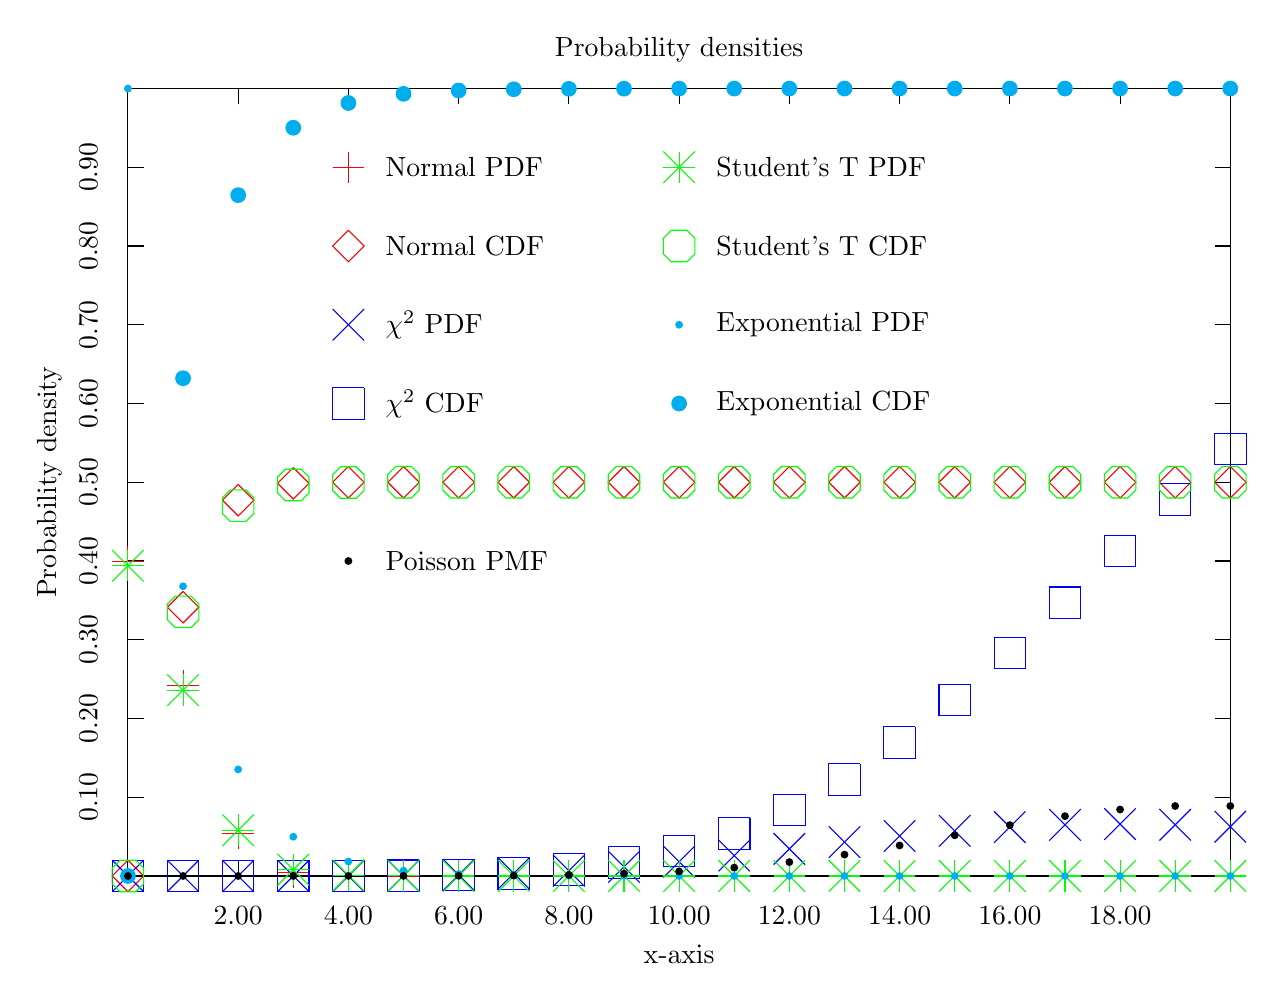
\begin{tikzpicture}
\draw ( 1.00000E+00, 1.00000E+00) rectangle ( 1.50000E+01, 1.10000E+01);
\draw ( 2.40000E+00, 1.00000E+00) -- ( 2.40000E+00, 1.20000E+00);
\draw ( 2.40000E+00, 1.08000E+01) -- ( 2.40000E+00, 1.10000E+01);
\node at ( 2.40000E+00, 5.00000E-01) { 2.00};
\draw ( 3.80000E+00, 1.00000E+00) -- ( 3.80000E+00, 1.20000E+00);
\draw ( 3.80000E+00, 1.08000E+01) -- ( 3.80000E+00, 1.10000E+01);
\node at ( 3.80000E+00, 5.00000E-01) { 4.00};
\draw ( 5.20000E+00, 1.00000E+00) -- ( 5.20000E+00, 1.20000E+00);
\draw ( 5.20000E+00, 1.08000E+01) -- ( 5.20000E+00, 1.10000E+01);
\node at ( 5.20000E+00, 5.00000E-01) { 6.00};
\draw ( 6.60000E+00, 1.00000E+00) -- ( 6.60000E+00, 1.20000E+00);
\draw ( 6.60000E+00, 1.08000E+01) -- ( 6.60000E+00, 1.10000E+01);
\node at ( 6.60000E+00, 5.00000E-01) { 8.00};
\draw ( 8.00000E+00, 1.00000E+00) -- ( 8.00000E+00, 1.20000E+00);
\draw ( 8.00000E+00, 1.08000E+01) -- ( 8.00000E+00, 1.10000E+01);
\node at ( 8.00000E+00, 5.00000E-01) {10.00};
\draw ( 9.40000E+00, 1.00000E+00) -- ( 9.40000E+00, 1.20000E+00);
\draw ( 9.40000E+00, 1.08000E+01) -- ( 9.40000E+00, 1.10000E+01);
\node at ( 9.40000E+00, 5.00000E-01) {12.00};
\draw ( 1.08000E+01, 1.00000E+00) -- ( 1.08000E+01, 1.20000E+00);
\draw ( 1.08000E+01, 1.08000E+01) -- ( 1.08000E+01, 1.10000E+01);
\node at ( 1.08000E+01, 5.00000E-01) {14.00};
\draw ( 1.22000E+01, 1.00000E+00) -- ( 1.22000E+01, 1.20000E+00);
\draw ( 1.22000E+01, 1.08000E+01) -- ( 1.22000E+01, 1.10000E+01);
\node at ( 1.22000E+01, 5.00000E-01) {16.00};
\draw ( 1.36000E+01, 1.00000E+00) -- ( 1.36000E+01, 1.20000E+00);
\draw ( 1.36000E+01, 1.08000E+01) -- ( 1.36000E+01, 1.10000E+01);
\node at ( 1.36000E+01, 5.00000E-01) {18.00};
\draw ( 1.00000E+00, 2.00000E+00) -- ( 1.20000E+00, 2.00000E+00);\draw ( 1.48000E+01, 2.00000E+00) -- ( 1.50000E+01, 2.00000E+00);
\node [rotate=90] at ( 5.00000E-01, 2.00000E+00) { 0.10};
\draw ( 1.00000E+00, 3.00000E+00) -- ( 1.20000E+00, 3.00000E+00);\draw ( 1.48000E+01, 3.00000E+00) -- ( 1.50000E+01, 3.00000E+00);
\node [rotate=90] at ( 5.00000E-01, 3.00000E+00) { 0.20};
\draw ( 1.00000E+00, 4.00000E+00) -- ( 1.20000E+00, 4.00000E+00);\draw ( 1.48000E+01, 4.00000E+00) -- ( 1.50000E+01, 4.00000E+00);
\node [rotate=90] at ( 5.00000E-01, 4.00000E+00) { 0.30};
\draw ( 1.00000E+00, 5.00000E+00) -- ( 1.20000E+00, 5.00000E+00);\draw ( 1.48000E+01, 5.00000E+00) -- ( 1.50000E+01, 5.00000E+00);
\node [rotate=90] at ( 5.00000E-01, 5.00000E+00) { 0.40};
\draw ( 1.00000E+00, 6.00000E+00) -- ( 1.20000E+00, 6.00000E+00);\draw ( 1.48000E+01, 6.00000E+00) -- ( 1.50000E+01, 6.00000E+00);
\node [rotate=90] at ( 5.00000E-01, 6.00000E+00) { 0.50};
\draw ( 1.00000E+00, 7.00000E+00) -- ( 1.20000E+00, 7.00000E+00);\draw ( 1.48000E+01, 7.00000E+00) -- ( 1.50000E+01, 7.00000E+00);
\node [rotate=90] at ( 5.00000E-01, 7.00000E+00) { 0.60};
\draw ( 1.00000E+00, 8.00000E+00) -- ( 1.20000E+00, 8.00000E+00);\draw ( 1.48000E+01, 8.00000E+00) -- ( 1.50000E+01, 8.00000E+00);
\node [rotate=90] at ( 5.00000E-01, 8.00000E+00) { 0.70};
\draw ( 1.00000E+00, 9.00000E+00) -- ( 1.20000E+00, 9.00000E+00);\draw ( 1.48000E+01, 9.00000E+00) -- ( 1.50000E+01, 9.00000E+00);
\node [rotate=90] at ( 5.00000E-01, 9.00000E+00) { 0.80};
\draw ( 1.00000E+00, 1.00000E+01) -- ( 1.20000E+00, 1.00000E+01);\draw ( 1.48000E+01, 1.00000E+01) -- ( 1.50000E+01, 1.00000E+01);
\node [rotate=90] at ( 5.00000E-01, 1.00000E+01) { 0.90};
\node at ( 8.00000E+00, 0.00000E+00) {x-axis};
\node [rotate=90] at ( 0.00000E+00, 6.00000E+00) {Probability density};
\node at ( 8.00000E+00, 1.15000E+01) {Probability densities};
\draw[red] ( 8.00000E-01, 4.98942E+00) -- ( 1.20000E+00, 4.98942E+00);\draw[red] ( 1.00000E+00
, 4.78942E+00) -- ( 1.00000E+00, 5.18942E+00);
\draw [red] ( 1.00000E+00, 1.20000E+00) -- ( 8.00000E-01, 1.00000E+00) -- ( 1.00000E+00, 8.00000E-01) -- ( 1.20000E+00, 1.00000E+00) -- ( 1.00000E+00, 1.20000E+00);
\draw [blue] ( 8.00000E-01, 8.00000E-01) -- ( 1.20000E+00, 1.20000E+00);
\draw [blue] ( 1.20000E+00, 8.00000E-01) -- ( 8.00000E-01, 1.20000E+00);
\draw [blue] ( 1.20000E+00, 1.20000E+00) -- ( 8.00000E-01, 1.20000E+00) -- ( 8.00000E-01, 8.00000E-01) -- ( 1.20000E+00, 8.00000E-01) -- ( 1.20000E+00, 1.20000E+00);
\draw[green] ( 8.00000E-01, 4.93988E+00) -- ( 1.20000E+00, 4.93988E+00);\draw[green] ( 1.00000E+00
, 4.73988E+00) -- ( 1.00000E+00, 5.13988E+00);
\draw [green] ( 8.00000E-01, 4.73988E+00) -- ( 1.20000E+00, 5.13988E+00);
\draw [green] ( 1.20000E+00, 4.73988E+00) -- ( 8.00000E-01, 5.13988E+00);
\draw [green] ( 9.00000E-01, 1.20000E+00) -- ( 1.10000E+00, 1.20000E+00) -- ( 1.20000E+00, 1.10000E+00) -- ( 1.20000E+00, 9.00000E-01) -- ( 1.10000E+00, 8.00000E-01) -- ( 9.00000E-01, 8.00000E-01) -- ( 8.00000E-01, 9.00000E-01) -- ( 8.00000E-01, 1.10000E+00) -- ( 9.00000E-01, 1.20000E+00);\path [fill=cyan] ( 1.00000E+00, 1.10000E+01) circle [radius= 5.00000E-02];
\path [fill=cyan] ( 1.00000E+00, 1.00000E+00) circle [radius= 1.00000E-01];
\path [fill=black] ( 1.00000E+00, 1.00000E+00) circle [radius= 5.00000E-02];
\draw[red] ( 1.50000E+00, 3.41971E+00) -- ( 1.90000E+00, 3.41971E+00);\draw[red] ( 1.70000E+00
, 3.21971E+00) -- ( 1.70000E+00, 3.61971E+00);
\draw [red] ( 1.70000E+00, 4.61345E+00) -- ( 1.50000E+00, 4.41345E+00) -- ( 1.70000E+00, 4.21345E+00) -- ( 1.90000E+00, 4.41345E+00) -- ( 1.70000E+00, 4.61345E+00);
\draw [blue] ( 1.50000E+00, 8.00000E-01) -- ( 1.90000E+00, 1.20000E+00);
\draw [blue] ( 1.90000E+00, 8.00000E-01) -- ( 1.50000E+00, 1.20000E+00);
\draw [blue] ( 1.90000E+00, 1.20000E+00) -- ( 1.50000E+00, 1.20000E+00) -- ( 1.50000E+00, 8.00000E-01) -- ( 1.90000E+00, 8.00000E-01) -- ( 1.90000E+00, 1.20000E+00);
\draw[green] ( 1.50000E+00, 3.36045E+00) -- ( 1.90000E+00, 3.36045E+00);\draw[green] ( 1.70000E+00
, 3.16045E+00) -- ( 1.70000E+00, 3.56045E+00);
\draw [green] ( 1.50000E+00, 3.16045E+00) -- ( 1.90000E+00, 3.56045E+00);
\draw [green] ( 1.90000E+00, 3.16045E+00) -- ( 1.50000E+00, 3.56045E+00);
\draw [green] ( 1.60000E+00, 4.55372E+00) -- ( 1.80000E+00, 4.55372E+00) -- ( 1.90000E+00, 4.45372E+00) -- ( 1.90000E+00, 4.25372E+00) -- ( 1.80000E+00, 4.15372E+00) -- ( 1.60000E+00, 4.15372E+00) -- ( 1.50000E+00, 4.25372E+00) -- ( 1.50000E+00, 4.45372E+00) -- ( 1.60000E+00, 4.55372E+00);\path [fill=cyan] ( 1.70000E+00, 4.67879E+00) circle [radius= 5.00000E-02];
\path [fill=cyan] ( 1.70000E+00, 7.32121E+00) circle [radius= 1.00000E-01];
\path [fill=black] ( 1.70000E+00, 1.00000E+00) circle [radius= 5.00000E-02];
\draw[red] ( 2.20000E+00, 1.53991E+00) -- ( 2.60000E+00, 1.53991E+00);\draw[red] ( 2.40000E+00
, 1.33991E+00) -- ( 2.40000E+00, 1.73991E+00);
\draw [red] ( 2.40000E+00, 5.97250E+00) -- ( 2.20000E+00, 5.77250E+00) -- ( 2.40000E+00, 5.57250E+00) -- ( 2.60000E+00, 5.77250E+00) -- ( 2.40000E+00, 5.97250E+00);
\draw [blue] ( 2.20000E+00, 8.00005E-01) -- ( 2.60000E+00, 1.20001E+00);
\draw [blue] ( 2.60000E+00, 8.00005E-01) -- ( 2.20000E+00, 1.20001E+00);
\draw [blue] ( 2.60000E+00, 1.20000E+00) -- ( 2.20000E+00, 1.20000E+00) -- ( 2.20000E+00, 8.00001E-01) -- ( 2.60000E+00, 8.00001E-01) -- ( 2.60000E+00, 1.20000E+00);
\draw[green] ( 2.20000E+00, 1.58087E+00) -- ( 2.60000E+00, 1.58087E+00);\draw[green] ( 2.40000E+00
, 1.38087E+00) -- ( 2.40000E+00, 1.78087E+00);
\draw [green] ( 2.20000E+00, 1.38087E+00) -- ( 2.60000E+00, 1.78087E+00);
\draw [green] ( 2.60000E+00, 1.38087E+00) -- ( 2.20000E+00, 1.78087E+00);
\draw [green] ( 2.30000E+00, 5.90366E+00) -- ( 2.50000E+00, 5.90366E+00) -- ( 2.60000E+00, 5.80366E+00) -- ( 2.60000E+00, 5.60366E+00) -- ( 2.50000E+00, 5.50366E+00) -- ( 2.30000E+00, 5.50366E+00) -- ( 2.20000E+00, 5.60366E+00) -- ( 2.20000E+00, 5.80366E+00) -- ( 2.30000E+00, 5.90366E+00);\path [fill=cyan] ( 2.40000E+00, 2.35335E+00) circle [radius= 5.00000E-02];
\path [fill=cyan] ( 2.40000E+00, 9.64665E+00) circle [radius= 1.00000E-01];
\path [fill=black] ( 2.40000E+00, 1.00000E+00) circle [radius= 5.00000E-02];
\draw[red] ( 2.90000E+00, 1.04432E+00) -- ( 3.30000E+00, 1.04432E+00);\draw[red] ( 3.10000E+00
, 8.44318E-01) -- ( 3.10000E+00, 1.24432E+00);
\draw [red] ( 3.10000E+00, 6.18650E+00) -- ( 2.90000E+00, 5.98650E+00) -- ( 3.10000E+00, 5.78650E+00) -- ( 3.30000E+00, 5.98650E+00) -- ( 3.10000E+00, 6.18650E+00);
\draw [blue] ( 2.90000E+00, 8.00118E-01) -- ( 3.30000E+00, 1.20012E+00);
\draw [blue] ( 3.30000E+00, 8.00118E-01) -- ( 2.90000E+00, 1.20012E+00);
\draw [blue] ( 3.30000E+00, 1.20004E+00) -- ( 2.90000E+00, 1.20004E+00) -- ( 2.90000E+00, 8.00043E-01) -- ( 3.30000E+00, 8.00043E-01) -- ( 3.30000E+00, 1.20004E+00);
\draw[green] ( 2.90000E+00, 1.07964E+00) -- ( 3.30000E+00, 1.07964E+00);\draw[green] ( 3.10000E+00
, 8.79638E-01) -- ( 3.10000E+00, 1.27964E+00);
\draw [green] ( 2.90000E+00, 8.79638E-01) -- ( 3.30000E+00, 1.27964E+00);
\draw [green] ( 3.30000E+00, 8.79638E-01) -- ( 2.90000E+00, 1.27964E+00);
\draw [green] ( 3.00000E+00, 6.16460E+00) -- ( 3.20000E+00, 6.16460E+00) -- ( 3.30000E+00, 6.06460E+00) -- ( 3.30000E+00, 5.86460E+00) -- ( 3.20000E+00, 5.76461E+00) -- ( 3.00000E+00, 5.76461E+00) -- ( 2.90000E+00, 5.86460E+00) -- ( 2.90000E+00, 6.06460E+00) -- ( 3.00000E+00, 6.16460E+00);\path [fill=cyan] ( 3.10000E+00, 1.49787E+00) circle [radius= 5.00000E-02];
\path [fill=cyan] ( 3.10000E+00, 1.05021E+01) circle [radius= 1.00000E-01];
\path [fill=black] ( 3.10000E+00, 1.00003E+00) circle [radius= 5.00000E-02];
\draw[red] ( 3.60000E+00, 1.00134E+00) -- ( 4.00000E+00, 1.00134E+00);\draw[red] ( 3.80000E+00
, 8.01338E-01) -- ( 3.80000E+00, 1.20134E+00);
\draw [red] ( 3.80000E+00, 6.19968E+00) -- ( 3.60000E+00, 5.99968E+00) -- ( 3.80000E+00, 5.79968E+00) -- ( 4.00000E+00, 5.99968E+00) -- ( 3.80000E+00, 6.19968E+00);
\draw [blue] ( 3.60000E+00, 8.00955E-01) -- ( 4.00000E+00, 1.20095E+00);
\draw [blue] ( 4.00000E+00, 8.00955E-01) -- ( 3.60000E+00, 1.20095E+00);
\draw [blue] ( 4.00000E+00, 1.20048E+00) -- ( 3.60000E+00, 1.20048E+00) -- ( 3.60000E+00, 8.00479E-01) -- ( 4.00000E+00, 8.00479E-01) -- ( 4.00000E+00, 1.20048E+00);
\draw[green] ( 3.60000E+00, 1.00822E+00) -- ( 4.00000E+00, 1.00822E+00);\draw[green] ( 3.80000E+00
, 8.08225E-01) -- ( 3.80000E+00, 1.20822E+00);
\draw [green] ( 3.60000E+00, 8.08225E-01) -- ( 4.00000E+00, 1.20822E+00);
\draw [green] ( 4.00000E+00, 8.08225E-01) -- ( 3.60000E+00, 1.20822E+00);
\draw [green] ( 3.70000E+00, 6.19649E+00) -- ( 3.90000E+00, 6.19649E+00) -- ( 4.00000E+00, 6.09649E+00) -- ( 4.00000E+00, 5.89649E+00) -- ( 3.90000E+00, 5.79649E+00) -- ( 3.70000E+00, 5.79649E+00) -- ( 3.60000E+00, 5.89649E+00) -- ( 3.60000E+00, 6.09649E+00) -- ( 3.70000E+00, 6.19649E+00);\path [fill=cyan] ( 3.80000E+00, 1.18316E+00) circle [radius= 5.00000E-02];
\path [fill=cyan] ( 3.80000E+00, 1.08168E+01) circle [radius= 1.00000E-01];
\path [fill=black] ( 3.80000E+00, 1.00014E+00) circle [radius= 5.00000E-02];
\draw[red] ( 4.30000E+00, 1.00001E+00) -- ( 4.70000E+00, 1.00001E+00);\draw[red] ( 4.50000E+00
, 8.00015E-01) -- ( 4.50000E+00, 1.20001E+00);
\draw [red] ( 4.50000E+00, 6.20000E+00) -- ( 4.30000E+00, 6.00000E+00) -- ( 4.50000E+00, 5.80000E+00) -- ( 4.70000E+00, 6.00000E+00) -- ( 4.50000E+00, 6.20000E+00);
\draw [blue] ( 4.30000E+00, 8.04315E-01) -- ( 4.70000E+00, 1.20431E+00);
\draw [blue] ( 4.70000E+00, 8.04315E-01) -- ( 4.30000E+00, 1.20431E+00);
\draw [blue] ( 4.70000E+00, 1.20283E+00) -- ( 4.30000E+00, 1.20283E+00) -- ( 4.30000E+00, 8.02831E-01) -- ( 4.70000E+00, 8.02831E-01) -- ( 4.70000E+00, 1.20283E+00);
\draw[green] ( 4.30000E+00, 1.00079E+00) -- ( 4.70000E+00, 1.00079E+00);\draw[green] ( 4.50000E+00
, 8.00790E-01) -- ( 4.50000E+00, 1.20079E+00);
\draw [green] ( 4.30000E+00, 8.00790E-01) -- ( 4.70000E+00, 1.20079E+00);
\draw [green] ( 4.70000E+00, 8.00790E-01) -- ( 4.30000E+00, 1.20079E+00);
\draw [green] ( 4.40000E+00, 6.19966E+00) -- ( 4.60000E+00, 6.19966E+00) -- ( 4.70000E+00, 6.09966E+00) -- ( 4.70000E+00, 5.89966E+00) -- ( 4.60000E+00, 5.79966E+00) -- ( 4.40000E+00, 5.79966E+00) -- ( 4.30000E+00, 5.89966E+00) -- ( 4.30000E+00, 6.09966E+00) -- ( 4.40000E+00, 6.19966E+00);\path [fill=cyan] ( 4.50000E+00, 1.06738E+00) circle [radius= 5.00000E-02];
\path [fill=cyan] ( 4.50000E+00, 1.09326E+01) circle [radius= 1.00000E-01];
\path [fill=black] ( 4.50000E+00, 1.00055E+00) circle [radius= 5.00000E-02];
\draw[red] ( 5.00000E+00, 1.00000E+00) -- ( 5.40000E+00, 1.00000E+00);\draw[red] ( 5.20000E+00
, 8.00000E-01) -- ( 5.20000E+00, 1.20000E+00);
\draw [red] ( 5.20000E+00, 6.20000E+00) -- ( 5.00000E+00, 6.00000E+00) -- ( 5.20000E+00, 5.80000E+00) -- ( 5.40000E+00, 6.00000E+00) -- ( 5.20000E+00, 6.20000E+00);
\draw [blue] ( 5.00000E+00, 8.13502E-01) -- ( 5.40000E+00, 1.21350E+00);
\draw [blue] ( 5.40000E+00, 8.13502E-01) -- ( 5.00000E+00, 1.21350E+00);
\draw [blue] ( 5.40000E+00, 1.21103E+00) -- ( 5.00000E+00, 1.21103E+00) -- ( 5.00000E+00, 8.11033E-01) -- ( 5.40000E+00, 8.11033E-01) -- ( 5.40000E+00, 1.21103E+00);
\draw[green] ( 5.00000E+00, 1.00008E+00) -- ( 5.40000E+00, 1.00008E+00);\draw[green] ( 5.20000E+00
, 8.00080E-01) -- ( 5.20000E+00, 1.20008E+00);
\draw [green] ( 5.00000E+00, 8.00080E-01) -- ( 5.40000E+00, 1.20008E+00);
\draw [green] ( 5.40000E+00, 8.00080E-01) -- ( 5.00000E+00, 1.20008E+00);
\draw [green] ( 5.10000E+00, 6.19997E+00) -- ( 5.30000E+00, 6.19997E+00) -- ( 5.40000E+00, 6.09997E+00) -- ( 5.40000E+00, 5.89997E+00) -- ( 5.30000E+00, 5.79997E+00) -- ( 5.10000E+00, 5.79997E+00) -- ( 5.00000E+00, 5.89997E+00) -- ( 5.00000E+00, 6.09997E+00) -- ( 5.10000E+00, 6.19997E+00);\path [fill=cyan] ( 5.20000E+00, 1.02479E+00) circle [radius= 5.00000E-02];
\path [fill=cyan] ( 5.20000E+00, 1.09752E+01) circle [radius= 1.00000E-01];
\path [fill=black] ( 5.20000E+00, 1.00183E+00) circle [radius= 5.00000E-02];
\draw[red] ( 5.70000E+00, 1.00000E+00) -- ( 6.10000E+00, 1.00000E+00);\draw[red] ( 5.90000E+00
, 8.00000E-01) -- ( 5.90000E+00, 1.20000E+00);
\draw [red] ( 5.90000E+00, 6.20000E+00) -- ( 5.70000E+00, 6.00000E+00) -- ( 5.90000E+00, 5.80000E+00) -- ( 6.10000E+00, 6.00000E+00) -- ( 5.90000E+00, 6.20000E+00);
\draw [blue] ( 5.70000E+00, 8.32794E-01) -- ( 6.10000E+00, 1.23279E+00);
\draw [blue] ( 6.10000E+00, 8.32794E-01) -- ( 5.70000E+00, 1.23279E+00);
\draw [blue] ( 6.10000E+00, 1.23316E+00) -- ( 5.70000E+00, 1.23316E+00) -- ( 5.70000E+00, 8.33161E-01) -- ( 6.10000E+00, 8.33161E-01) -- ( 6.10000E+00, 1.23316E+00);
\draw[green] ( 5.70000E+00, 1.00001E+00) -- ( 6.10000E+00, 1.00001E+00);\draw[green] ( 5.90000E+00
, 8.00009E-01) -- ( 5.90000E+00, 1.20001E+00);
\draw [green] ( 5.70000E+00, 8.00009E-01) -- ( 6.10000E+00, 1.20001E+00);
\draw [green] ( 6.10000E+00, 8.00009E-01) -- ( 5.70000E+00, 1.20001E+00);
\draw [green] ( 5.80000E+00, 6.19998E+00) -- ( 6.00000E+00, 6.19998E+00) -- ( 6.10000E+00, 6.09998E+00) -- ( 6.10000E+00, 5.89998E+00) -- ( 6.00000E+00, 5.79998E+00) -- ( 5.80000E+00, 5.79998E+00) -- ( 5.70000E+00, 5.89998E+00) -- ( 5.70000E+00, 6.09998E+00) -- ( 5.80000E+00, 6.19998E+00);\path [fill=cyan] ( 5.90000E+00, 1.00912E+00) circle [radius= 5.00000E-02];
\path [fill=cyan] ( 5.90000E+00, 1.09909E+01) circle [radius= 1.00000E-01];
\path [fill=black] ( 5.90000E+00, 1.00523E+00) circle [radius= 5.00000E-02];
\draw[red] ( 6.40000E+00, 1.00000E+00) -- ( 6.80000E+00, 1.00000E+00);\draw[red] ( 6.60000E+00
, 8.00000E-01) -- ( 6.60000E+00, 1.20000E+00);
\draw [red] ( 6.60000E+00, 6.20000E+00) -- ( 6.40000E+00, 6.00000E+00) -- ( 6.60000E+00, 5.80000E+00) -- ( 6.80000E+00, 6.00000E+00) -- ( 6.60000E+00, 6.20000E+00);
\draw [blue] ( 6.40000E+00, 8.66156E-01) -- ( 6.80000E+00, 1.26616E+00);
\draw [blue] ( 6.80000E+00, 8.66156E-01) -- ( 6.40000E+00, 1.26616E+00);
\draw [blue] ( 6.80000E+00, 1.28133E+00) -- ( 6.40000E+00, 1.28133E+00) -- ( 6.40000E+00, 8.81329E-01) -- ( 6.80000E+00, 8.81329E-01) -- ( 6.80000E+00, 1.28133E+00);
\draw[green] ( 6.40000E+00, 1.00000E+00) -- ( 6.80000E+00, 1.00000E+00);\draw[green] ( 6.60000E+00
, 8.00001E-01) -- ( 6.60000E+00, 1.20000E+00);
\draw [green] ( 6.40000E+00, 8.00001E-01) -- ( 6.80000E+00, 1.20000E+00);
\draw [green] ( 6.80000E+00, 8.00001E-01) -- ( 6.40000E+00, 1.20000E+00);
\draw [green] ( 6.50000E+00, 6.19999E+00) -- ( 6.70000E+00, 6.19999E+00) -- ( 6.80000E+00, 6.09999E+00) -- ( 6.80000E+00, 5.89999E+00) -- ( 6.70000E+00, 5.79999E+00) -- ( 6.50000E+00, 5.79999E+00) -- ( 6.40000E+00, 5.89999E+00) -- ( 6.40000E+00, 6.09999E+00) -- ( 6.50000E+00, 6.19999E+00);\path [fill=cyan] ( 6.60000E+00, 1.00335E+00) circle [radius= 5.00000E-02];
\path [fill=cyan] ( 6.60000E+00, 1.09966E+01) circle [radius= 1.00000E-01];
\path [fill=black] ( 6.60000E+00, 1.01309E+00) circle [radius= 5.00000E-02];
\draw[red] ( 7.10000E+00, 1.00000E+00) -- ( 7.50000E+00, 1.00000E+00);\draw[red] ( 7.30000E+00
, 8.00000E-01) -- ( 7.30000E+00, 1.20000E+00);
\draw [red] ( 7.30000E+00, 6.20000E+00) -- ( 7.10000E+00, 6.00000E+00) -- ( 7.30000E+00, 5.80000E+00) -- ( 7.50000E+00, 6.00000E+00) -- ( 7.30000E+00, 6.20000E+00);
\draw [blue] ( 7.10000E+00, 9.15823E-01) -- ( 7.50000E+00, 1.31582E+00);
\draw [blue] ( 7.50000E+00, 9.15823E-01) -- ( 7.10000E+00, 1.31582E+00);
\draw [blue] ( 7.50000E+00, 1.37096E+00) -- ( 7.10000E+00, 1.37096E+00) -- ( 7.10000E+00, 9.70955E-01) -- ( 7.50000E+00, 9.70955E-01) -- ( 7.50000E+00, 1.37096E+00);
\draw[green] ( 7.10000E+00, 1.00000E+00) -- ( 7.50000E+00, 1.00000E+00);\draw[green] ( 7.30000E+00
, 8.00000E-01) -- ( 7.30000E+00, 1.20000E+00);
\draw [green] ( 7.10000E+00, 8.00000E-01) -- ( 7.50000E+00, 1.20000E+00);
\draw [green] ( 7.50000E+00, 8.00000E-01) -- ( 7.10000E+00, 1.20000E+00);
\draw [green] ( 7.20000E+00, 6.20001E+00) -- ( 7.40000E+00, 6.20001E+00) -- ( 7.50000E+00, 6.10001E+00) -- ( 7.50000E+00, 5.90001E+00) -- ( 7.40000E+00, 5.80001E+00) -- ( 7.20000E+00, 5.80001E+00) -- ( 7.10000E+00, 5.90001E+00) -- ( 7.10000E+00, 6.10001E+00) -- ( 7.20000E+00, 6.20001E+00);\path [fill=cyan] ( 7.30000E+00, 1.00123E+00) circle [radius= 5.00000E-02];
\path [fill=cyan] ( 7.30000E+00, 1.09988E+01) circle [radius= 1.00000E-01];
\path [fill=black] ( 7.30000E+00, 1.02908E+00) circle [radius= 5.00000E-02];
\draw[red] ( 7.80000E+00, 1.00000E+00) -- ( 8.20000E+00, 1.00000E+00);\draw[red] ( 8.00000E+00
, 8.00000E-01) -- ( 8.00000E+00, 1.20000E+00);
\draw [red] ( 8.00000E+00, 6.20000E+00) -- ( 7.80000E+00, 6.00000E+00) -- ( 8.00000E+00, 5.80000E+00) -- ( 8.20000E+00, 6.00000E+00) -- ( 8.00000E+00, 6.20000E+00);
\draw [blue] ( 7.80000E+00, 9.81328E-01) -- ( 8.20000E+00, 1.38133E+00);
\draw [blue] ( 8.20000E+00, 9.81328E-01) -- ( 7.80000E+00, 1.38133E+00);
\draw [blue] ( 8.20000E+00, 1.51828E+00) -- ( 7.80000E+00, 1.51828E+00) -- ( 7.80000E+00, 1.11828E+00) -- ( 8.20000E+00, 1.11828E+00) -- ( 8.20000E+00, 1.51828E+00);
\draw[green] ( 7.80000E+00, 1.00000E+00) -- ( 8.20000E+00, 1.00000E+00);\draw[green] ( 8.00000E+00
, 8.00000E-01) -- ( 8.00000E+00, 1.20000E+00);
\draw [green] ( 7.80000E+00, 8.00000E-01) -- ( 8.20000E+00, 1.20000E+00);
\draw [green] ( 8.20000E+00, 8.00000E-01) -- ( 7.80000E+00, 1.20000E+00);
\draw [green] ( 7.90000E+00, 6.20007E+00) -- ( 8.10000E+00, 6.20007E+00) -- ( 8.20000E+00, 6.10007E+00) -- ( 8.20000E+00, 5.90007E+00) -- ( 8.10000E+00, 5.80007E+00) -- ( 7.90000E+00, 5.80007E+00) -- ( 7.80000E+00, 5.90007E+00) -- ( 7.80000E+00, 6.10007E+00) -- ( 7.90000E+00, 6.20007E+00);\path [fill=cyan] ( 8.00000E+00, 1.00045E+00) circle [radius= 5.00000E-02];
\path [fill=cyan] ( 8.00000E+00, 1.09995E+01) circle [radius= 1.00000E-01];
\path [fill=black] ( 8.00000E+00, 1.05816E+00) circle [radius= 5.00000E-02];
\draw[red] ( 8.50000E+00, 1.00000E+00) -- ( 8.90000E+00, 1.00000E+00);\draw[red] ( 8.70000E+00
, 8.00000E-01) -- ( 8.70000E+00, 1.20000E+00);
\draw [red] ( 8.70000E+00, 6.20000E+00) -- ( 8.50000E+00, 6.00000E+00) -- ( 8.70000E+00, 5.80000E+00) -- ( 8.90000E+00, 6.00000E+00) -- ( 8.70000E+00, 6.20000E+00);
\draw [blue] ( 8.50000E+00, 1.05933E+00) -- ( 8.90000E+00, 1.45933E+00);
\draw [blue] ( 8.90000E+00, 1.05933E+00) -- ( 8.50000E+00, 1.45933E+00);
\draw [blue] ( 8.90000E+00, 1.73777E+00) -- ( 8.50000E+00, 1.73777E+00) -- ( 8.50000E+00, 1.33777E+00) -- ( 8.90000E+00, 1.33777E+00) -- ( 8.90000E+00, 1.73777E+00);
\draw[green] ( 8.50000E+00, 1.00000E+00) -- ( 8.90000E+00, 1.00000E+00);\draw[green] ( 8.70000E+00
, 8.00000E-01) -- ( 8.70000E+00, 1.20000E+00);
\draw [green] ( 8.50000E+00, 8.00000E-01) -- ( 8.90000E+00, 1.20000E+00);
\draw [green] ( 8.90000E+00, 8.00000E-01) -- ( 8.50000E+00, 1.20000E+00);
\draw [green] ( 8.60000E+00, 6.20003E+00) -- ( 8.80000E+00, 6.20003E+00) -- ( 8.90000E+00, 6.10003E+00) -- ( 8.90000E+00, 5.90003E+00) -- ( 8.80000E+00, 5.80003E+00) -- ( 8.60000E+00, 5.80003E+00) -- ( 8.50000E+00, 5.90003E+00) -- ( 8.50000E+00, 6.10003E+00) -- ( 8.60000E+00, 6.20003E+00);\path [fill=cyan] ( 8.70000E+00, 1.00017E+00) circle [radius= 5.00000E-02];
\path [fill=cyan] ( 8.70000E+00, 1.09998E+01) circle [radius= 1.00000E-01];
\path [fill=black] ( 8.70000E+00, 1.10575E+00) circle [radius= 5.00000E-02];
\draw[red] ( 9.20000E+00, 1.00000E+00) -- ( 9.60000E+00, 1.00000E+00);\draw[red] ( 9.40000E+00
, 8.00000E-01) -- ( 9.40000E+00, 1.20000E+00);
\draw [red] ( 9.40000E+00, 6.20000E+00) -- ( 9.20000E+00, 6.00000E+00) -- ( 9.40000E+00, 5.80000E+00) -- ( 9.60000E+00, 6.00000E+00) -- ( 9.40000E+00, 6.20000E+00);
\draw [blue] ( 9.20000E+00, 1.14419E+00) -- ( 9.60000E+00, 1.54419E+00);
\draw [blue] ( 9.60000E+00, 1.14419E+00) -- ( 9.20000E+00, 1.54419E+00);
\draw [blue] ( 9.60000E+00, 2.03923E+00) -- ( 9.20000E+00, 2.03923E+00) -- ( 9.20000E+00, 1.63923E+00) -- ( 9.60000E+00, 1.63923E+00) -- ( 9.60000E+00, 2.03923E+00);
\draw[green] ( 9.20000E+00, 1.00000E+00) -- ( 9.60000E+00, 1.00000E+00);\draw[green] ( 9.40000E+00
, 8.00000E-01) -- ( 9.40000E+00, 1.20000E+00);
\draw [green] ( 9.20000E+00, 8.00000E-01) -- ( 9.60000E+00, 1.20000E+00);
\draw [green] ( 9.60000E+00, 8.00000E-01) -- ( 9.20000E+00, 1.20000E+00);
\draw [green] ( 9.30000E+00, 6.20001E+00) -- ( 9.50000E+00, 6.20001E+00) -- ( 9.60000E+00, 6.10001E+00) -- ( 9.60000E+00, 5.90001E+00) -- ( 9.50000E+00, 5.80001E+00) -- ( 9.30000E+00, 5.80001E+00) -- ( 9.20000E+00, 5.90001E+00) -- ( 9.20000E+00, 6.10001E+00) -- ( 9.30000E+00, 6.20001E+00);\path [fill=cyan] ( 9.40000E+00, 1.00006E+00) circle [radius= 5.00000E-02];
\path [fill=cyan] ( 9.40000E+00, 1.09999E+01) circle [radius= 1.00000E-01];
\path [fill=black] ( 9.40000E+00, 1.17625E+00) circle [radius= 5.00000E-02];
\draw[red] ( 9.90000E+00, 1.00000E+00) -- ( 1.03000E+01, 1.00000E+00);\draw[red] ( 1.01000E+01
, 8.00000E-01) -- ( 1.01000E+01, 1.20000E+00);
\draw [red] ( 1.01000E+01, 6.20000E+00) -- ( 9.90000E+00, 6.00000E+00) -- ( 1.01000E+01, 5.80000E+00) -- ( 1.03000E+01, 6.00000E+00) -- ( 1.01000E+01, 6.20000E+00);
\draw [blue] ( 9.90000E+00, 1.22906E+00) -- ( 1.03000E+01, 1.62906E+00);
\draw [blue] ( 1.03000E+01, 1.22906E+00) -- ( 9.90000E+00, 1.62906E+00);
\draw [blue] ( 1.03000E+01, 2.42616E+00) -- ( 9.90000E+00, 2.42616E+00) -- ( 9.90000E+00, 2.02616E+00) -- ( 1.03000E+01, 2.02616E+00) -- ( 1.03000E+01, 2.42616E+00);
\draw[green] ( 9.90000E+00, 1.00000E+00) -- ( 1.03000E+01, 1.00000E+00);\draw[green] ( 1.01000E+01
, 8.00000E-01) -- ( 1.01000E+01, 1.20000E+00);
\draw [green] ( 9.90000E+00, 8.00000E-01) -- ( 1.03000E+01, 1.20000E+00);
\draw [green] ( 1.03000E+01, 8.00000E-01) -- ( 9.90000E+00, 1.20000E+00);
\draw [green] ( 1.00000E+01, 6.20000E+00) -- ( 1.02000E+01, 6.20000E+00) -- ( 1.03000E+01, 6.10000E+00) -- ( 1.03000E+01, 5.90000E+00) -- ( 1.02000E+01, 5.80000E+00) -- ( 1.00000E+01, 5.80000E+00) -- ( 9.90000E+00, 5.90000E+00) -- ( 9.90000E+00, 6.10000E+00) -- ( 1.00000E+01, 6.20000E+00);\path [fill=cyan] ( 1.01000E+01, 1.00002E+00) circle [radius= 5.00000E-02];
\path [fill=cyan] ( 1.01000E+01, 1.10000E+01) circle [radius= 1.00000E-01];
\path [fill=black] ( 1.01000E+01, 1.27116E+00) circle [radius= 5.00000E-02];
\draw[red] ( 1.06000E+01, 1.00000E+00) -- ( 1.10000E+01, 1.00000E+00);\draw[red] ( 1.08000E+01
, 8.00000E-01) -- ( 1.08000E+01, 1.20000E+00);
\draw [red] ( 1.08000E+01, 6.20000E+00) -- ( 1.06000E+01, 6.00000E+00) -- ( 1.08000E+01, 5.80000E+00) -- ( 1.10000E+01, 6.00000E+00) -- ( 1.08000E+01, 6.20000E+00);
\draw [blue] ( 1.06000E+01, 1.30702E+00) -- ( 1.10000E+01, 1.70702E+00);
\draw [blue] ( 1.10000E+01, 1.30702E+00) -- ( 1.06000E+01, 1.70702E+00);
\draw [blue] ( 1.10000E+01, 2.89505E+00) -- ( 1.06000E+01, 2.89505E+00) -- ( 1.06000E+01, 2.49505E+00) -- ( 1.10000E+01, 2.49505E+00) -- ( 1.10000E+01, 2.89505E+00);
\draw[green] ( 1.06000E+01, 1.00000E+00) -- ( 1.10000E+01, 1.00000E+00);\draw[green] ( 1.08000E+01
, 8.00000E-01) -- ( 1.08000E+01, 1.20000E+00);
\draw [green] ( 1.06000E+01, 8.00000E-01) -- ( 1.10000E+01, 1.20000E+00);
\draw [green] ( 1.10000E+01, 8.00000E-01) -- ( 1.06000E+01, 1.20000E+00);
\draw [green] ( 1.07000E+01, 6.19999E+00) -- ( 1.09000E+01, 6.19999E+00) -- ( 1.10000E+01, 6.09999E+00) -- ( 1.10000E+01, 5.89999E+00) -- ( 1.09000E+01, 5.79999E+00) -- ( 1.07000E+01, 5.79999E+00) -- ( 1.06000E+01, 5.89999E+00) -- ( 1.06000E+01, 6.09999E+00) -- ( 1.07000E+01, 6.19999E+00);\path [fill=cyan] ( 1.08000E+01, 1.00001E+00) circle [radius= 5.00000E-02];
\path [fill=cyan] ( 1.08000E+01, 1.10000E+01) circle [radius= 1.00000E-01];
\path [fill=black] ( 1.08000E+01, 1.38737E+00) circle [radius= 5.00000E-02];
\draw[red] ( 1.13000E+01, 1.00000E+00) -- ( 1.17000E+01, 1.00000E+00);\draw[red] ( 1.15000E+01
, 8.00000E-01) -- ( 1.15000E+01, 1.20000E+00);
\draw [red] ( 1.15000E+01, 6.20000E+00) -- ( 1.13000E+01, 6.00000E+00) -- ( 1.15000E+01, 5.80000E+00) -- ( 1.17000E+01, 6.00000E+00) -- ( 1.15000E+01, 6.20000E+00);
\draw [blue] ( 1.13000E+01, 1.37220E+00) -- ( 1.17000E+01, 1.77220E+00);
\draw [blue] ( 1.17000E+01, 1.37220E+00) -- ( 1.13000E+01, 1.77220E+00);
\draw [blue] ( 1.17000E+01, 3.43593E+00) -- ( 1.13000E+01, 3.43593E+00) -- ( 1.13000E+01, 3.03593E+00) -- ( 1.17000E+01, 3.03593E+00) -- ( 1.17000E+01, 3.43593E+00);
\draw[green] ( 1.13000E+01, 1.00000E+00) -- ( 1.17000E+01, 1.00000E+00);\draw[green] ( 1.15000E+01
, 8.00000E-01) -- ( 1.15000E+01, 1.20000E+00);
\draw [green] ( 1.13000E+01, 8.00000E-01) -- ( 1.17000E+01, 1.20000E+00);
\draw [green] ( 1.17000E+01, 8.00000E-01) -- ( 1.13000E+01, 1.20000E+00);
\draw [green] ( 1.14000E+01, 6.20000E+00) -- ( 1.16000E+01, 6.20000E+00) -- ( 1.17000E+01, 6.10000E+00) -- ( 1.17000E+01, 5.90000E+00) -- ( 1.16000E+01, 5.80000E+00) -- ( 1.14000E+01, 5.80000E+00) -- ( 1.13000E+01, 5.90000E+00) -- ( 1.13000E+01, 6.10000E+00) -- ( 1.14000E+01, 6.20000E+00);\path [fill=cyan] ( 1.15000E+01, 1.00000E+00) circle [radius= 5.00000E-02];
\path [fill=cyan] ( 1.15000E+01, 1.10000E+01) circle [radius= 1.00000E-01];
\path [fill=black] ( 1.15000E+01, 1.51649E+00) circle [radius= 5.00000E-02];
\draw[red] ( 1.20000E+01, 1.00000E+00) -- ( 1.24000E+01, 1.00000E+00);\draw[red] ( 1.22000E+01
, 8.00000E-01) -- ( 1.22000E+01, 1.20000E+00);
\draw [red] ( 1.22000E+01, 6.20000E+00) -- ( 1.20000E+01, 6.00000E+00) -- ( 1.22000E+01, 5.80000E+00) -- ( 1.24000E+01, 6.00000E+00) -- ( 1.22000E+01, 6.20000E+00);
\draw [blue] ( 1.20000E+01, 1.42038E+00) -- ( 1.24000E+01, 1.82038E+00);
\draw [blue] ( 1.24000E+01, 1.42038E+00) -- ( 1.20000E+01, 1.82038E+00);
\draw [blue] ( 1.24000E+01, 4.03376E+00) -- ( 1.20000E+01, 4.03376E+00) -- ( 1.20000E+01, 3.63376E+00) -- ( 1.24000E+01, 3.63376E+00) -- ( 1.24000E+01, 4.03376E+00);
\draw[green] ( 1.20000E+01, 1.00000E+00) -- ( 1.24000E+01, 1.00000E+00);\draw[green] ( 1.22000E+01
, 8.00000E-01) -- ( 1.22000E+01, 1.20000E+00);
\draw [green] ( 1.20000E+01, 8.00000E-01) -- ( 1.24000E+01, 1.20000E+00);
\draw [green] ( 1.24000E+01, 8.00000E-01) -- ( 1.20000E+01, 1.20000E+00);
\draw [green] ( 1.21000E+01, 6.20000E+00) -- ( 1.23000E+01, 6.20000E+00) -- ( 1.24000E+01, 6.10000E+00) -- ( 1.24000E+01, 5.90000E+00) -- ( 1.23000E+01, 5.80000E+00) -- ( 1.21000E+01, 5.80000E+00) -- ( 1.20000E+01, 5.90000E+00) -- ( 1.20000E+01, 6.10000E+00) -- ( 1.21000E+01, 6.20000E+00);\path [fill=cyan] ( 1.22000E+01, 1.00000E+00) circle [radius= 5.00000E-02];
\path [fill=cyan] ( 1.22000E+01, 1.10000E+01) circle [radius= 1.00000E-01];
\path [fill=black] ( 1.22000E+01, 1.64561E+00) circle [radius= 5.00000E-02];
\draw[red] ( 1.27000E+01, 1.00000E+00) -- ( 1.31000E+01, 1.00000E+00);\draw[red] ( 1.29000E+01
, 8.00000E-01) -- ( 1.29000E+01, 1.20000E+00);
\draw [red] ( 1.29000E+01, 6.20000E+00) -- ( 1.27000E+01, 6.00000E+00) -- ( 1.29000E+01, 5.80000E+00) -- ( 1.31000E+01, 6.00000E+00) -- ( 1.29000E+01, 6.20000E+00);
\draw [blue] ( 1.27000E+01, 1.44934E+00) -- ( 1.31000E+01, 1.84934E+00);
\draw [blue] ( 1.31000E+01, 1.44934E+00) -- ( 1.27000E+01, 1.84934E+00);
\draw [blue] ( 1.31000E+01, 4.67026E+00) -- ( 1.27000E+01, 4.67026E+00) -- ( 1.27000E+01, 4.27026E+00) -- ( 1.31000E+01, 4.27026E+00) -- ( 1.31000E+01, 4.67026E+00);
\draw[green] ( 1.27000E+01, 1.00000E+00) -- ( 1.31000E+01, 1.00000E+00);\draw[green] ( 1.29000E+01
, 8.00000E-01) -- ( 1.29000E+01, 1.20000E+00);
\draw [green] ( 1.27000E+01, 8.00000E-01) -- ( 1.31000E+01, 1.20000E+00);
\draw [green] ( 1.31000E+01, 8.00000E-01) -- ( 1.27000E+01, 1.20000E+00);
\draw [green] ( 1.28000E+01, 6.20000E+00) -- ( 1.30000E+01, 6.20000E+00) -- ( 1.31000E+01, 6.10000E+00) -- ( 1.31000E+01, 5.90000E+00) -- ( 1.30000E+01, 5.80000E+00) -- ( 1.28000E+01, 5.80000E+00) -- ( 1.27000E+01, 5.90000E+00) -- ( 1.27000E+01, 6.10000E+00) -- ( 1.28000E+01, 6.20000E+00);\path [fill=cyan] ( 1.29000E+01, 1.00000E+00) circle [radius= 5.00000E-02];
\path [fill=cyan] ( 1.29000E+01, 1.10000E+01) circle [radius= 1.00000E-01];
\path [fill=black] ( 1.29000E+01, 1.75954E+00) circle [radius= 5.00000E-02];
\draw[red] ( 1.34000E+01, 1.00000E+00) -- ( 1.38000E+01, 1.00000E+00);\draw[red] ( 1.36000E+01
, 8.00000E-01) -- ( 1.36000E+01, 1.20000E+00);
\draw [red] ( 1.36000E+01, 6.20000E+00) -- ( 1.34000E+01, 6.00000E+00) -- ( 1.36000E+01, 5.80000E+00) -- ( 1.38000E+01, 6.00000E+00) -- ( 1.36000E+01, 6.20000E+00);
\draw [blue] ( 1.34000E+01, 1.45878E+00) -- ( 1.38000E+01, 1.85878E+00);
\draw [blue] ( 1.38000E+01, 1.45878E+00) -- ( 1.34000E+01, 1.85878E+00);
\draw [blue] ( 1.38000E+01, 5.32592E+00) -- ( 1.34000E+01, 5.32592E+00) -- ( 1.34000E+01, 4.92592E+00) -- ( 1.38000E+01, 4.92592E+00) -- ( 1.38000E+01, 5.32592E+00);
\draw[green] ( 1.34000E+01, 1.00000E+00) -- ( 1.38000E+01, 1.00000E+00);\draw[green] ( 1.36000E+01
, 8.00000E-01) -- ( 1.36000E+01, 1.20000E+00);
\draw [green] ( 1.34000E+01, 8.00000E-01) -- ( 1.38000E+01, 1.20000E+00);
\draw [green] ( 1.38000E+01, 8.00000E-01) -- ( 1.34000E+01, 1.20000E+00);
\draw [green] ( 1.35000E+01, 6.20000E+00) -- ( 1.37000E+01, 6.20000E+00) -- ( 1.38000E+01, 6.10000E+00) -- ( 1.38000E+01, 5.90000E+00) -- ( 1.37000E+01, 5.80000E+00) -- ( 1.35000E+01, 5.80000E+00) -- ( 1.34000E+01, 5.90000E+00) -- ( 1.34000E+01, 6.10000E+00) -- ( 1.35000E+01, 6.20000E+00);\path [fill=cyan] ( 1.36000E+01, 1.00000E+00) circle [radius= 5.00000E-02];
\path [fill=cyan] ( 1.36000E+01, 1.10000E+01) circle [radius= 1.00000E-01];
\path [fill=black] ( 1.36000E+01, 1.84393E+00) circle [radius= 5.00000E-02];
\draw[red] ( 1.41000E+01, 1.00000E+00) -- ( 1.45000E+01, 1.00000E+00);\draw[red] ( 1.43000E+01
, 8.00000E-01) -- ( 1.43000E+01, 1.20000E+00);
\draw [red] ( 1.43000E+01, 6.20000E+00) -- ( 1.41000E+01, 6.00000E+00) -- ( 1.43000E+01, 5.80000E+00) -- ( 1.45000E+01, 6.00000E+00) -- ( 1.43000E+01, 6.20000E+00);
\draw [blue] ( 1.41000E+01, 1.45001E+00) -- ( 1.45000E+01, 1.85001E+00);
\draw [blue] ( 1.45000E+01, 1.45001E+00) -- ( 1.41000E+01, 1.85001E+00);
\draw [blue] ( 1.45000E+01, 5.98173E+00) -- ( 1.41000E+01, 5.98173E+00) -- ( 1.41000E+01, 5.58173E+00) -- ( 1.45000E+01, 5.58173E+00) -- ( 1.45000E+01, 5.98173E+00);
\draw[green] ( 1.41000E+01, 1.00000E+00) -- ( 1.45000E+01, 1.00000E+00);\draw[green] ( 1.43000E+01
, 8.00000E-01) -- ( 1.43000E+01, 1.20000E+00);
\draw [green] ( 1.41000E+01, 8.00000E-01) -- ( 1.45000E+01, 1.20000E+00);
\draw [green] ( 1.45000E+01, 8.00000E-01) -- ( 1.41000E+01, 1.20000E+00);
\draw [green] ( 1.42000E+01, 6.20001E+00) -- ( 1.44000E+01, 6.20001E+00) -- ( 1.45000E+01, 6.10001E+00) -- ( 1.45000E+01, 5.90001E+00) -- ( 1.44000E+01, 5.80001E+00) -- ( 1.42000E+01, 5.80001E+00) -- ( 1.41000E+01, 5.90001E+00) -- ( 1.41000E+01, 6.10001E+00) -- ( 1.42000E+01, 6.20001E+00);\path [fill=cyan] ( 1.43000E+01, 1.00000E+00) circle [radius= 5.00000E-02];
\path [fill=cyan] ( 1.43000E+01, 1.10000E+01) circle [radius= 1.00000E-01];
\path [fill=black] ( 1.43000E+01, 1.88835E+00) circle [radius= 5.00000E-02];
\draw[red] ( 1.48000E+01, 1.00000E+00) -- ( 1.52000E+01, 1.00000E+00);\draw[red] ( 1.50000E+01
, 8.00000E-01) -- ( 1.50000E+01, 1.20000E+00);
\draw [red] ( 1.50000E+01, 6.20000E+00) -- ( 1.48000E+01, 6.00000E+00) -- ( 1.50000E+01, 5.80000E+00) -- ( 1.52000E+01, 6.00000E+00) -- ( 1.50000E+01, 6.20000E+00);
\draw [blue] ( 1.48000E+01, 1.42555E+00) -- ( 1.52000E+01, 1.82555E+00);
\draw [blue] ( 1.52000E+01, 1.42555E+00) -- ( 1.48000E+01, 1.82555E+00);
\draw [blue] ( 1.52000E+01, 6.62071E+00) -- ( 1.48000E+01, 6.62071E+00) -- ( 1.48000E+01, 6.22071E+00) -- ( 1.52000E+01, 6.22071E+00) -- ( 1.52000E+01, 6.62071E+00);
\draw[green] ( 1.48000E+01, 1.00000E+00) -- ( 1.52000E+01, 1.00000E+00);\draw[green] ( 1.50000E+01
, 8.00000E-01) -- ( 1.50000E+01, 1.20000E+00);
\draw [green] ( 1.48000E+01, 8.00000E-01) -- ( 1.52000E+01, 1.20000E+00);
\draw [green] ( 1.52000E+01, 8.00000E-01) -- ( 1.48000E+01, 1.20000E+00);
\draw [green] ( 1.49000E+01, 6.20000E+00) -- ( 1.51000E+01, 6.20000E+00) -- ( 1.52000E+01, 6.10000E+00) -- ( 1.52000E+01, 5.90000E+00) -- ( 1.51000E+01, 5.80000E+00) -- ( 1.49000E+01, 5.80000E+00) -- ( 1.48000E+01, 5.90000E+00) -- ( 1.48000E+01, 6.10000E+00) -- ( 1.49000E+01, 6.20000E+00);\path [fill=cyan] ( 1.50000E+01, 1.00000E+00) circle [radius= 5.00000E-02];
\path [fill=cyan] ( 1.50000E+01, 1.10000E+01) circle [radius= 1.00000E-01];
\path [fill=black] ( 1.50000E+01, 1.88835E+00) circle [radius= 5.00000E-02];
\draw[red] ( 3.60000E+00, 1.00000E+01) -- ( 4.00000E+00, 1.00000E+01);\draw[red] ( 3.80000E+00
, 9.80000E+00) -- ( 3.80000E+00, 1.02000E+01);
\node [right, black] at ( 4.15000E+00, 1.00000E+01) {Normal PDF};
\draw [red] ( 3.80000E+00, 9.20000E+00) -- ( 3.60000E+00, 9.00000E+00) -- ( 3.80000E+00, 8.80000E+00) -- ( 4.00000E+00, 9.00000E+00) -- ( 3.80000E+00, 9.20000E+00);
\node [right, black] at ( 4.15000E+00, 9.00000E+00) {Normal CDF};
\draw [blue] ( 3.60000E+00, 7.80000E+00) -- ( 4.00000E+00, 8.20000E+00);
\draw [blue] ( 4.00000E+00, 7.80000E+00) -- ( 3.60000E+00, 8.20000E+00);
\node [right, black] at ( 4.15000E+00, 8.00000E+00) {$\chi^2$ PDF};
\draw [blue] ( 4.00000E+00, 7.20000E+00) -- ( 3.60000E+00, 7.20000E+00) -- ( 3.60000E+00, 6.80000E+00) -- ( 4.00000E+00, 6.80000E+00) -- ( 4.00000E+00, 7.20000E+00);
\node [right, black] at ( 4.15000E+00, 7.00000E+00) {$\chi^2$ CDF};
\draw[green] ( 7.80000E+00, 1.00000E+01) -- ( 8.20000E+00, 1.00000E+01);\draw[green] ( 8.00000E+00
, 9.80000E+00) -- ( 8.00000E+00, 1.02000E+01);
\draw [green] ( 7.80000E+00, 9.80000E+00) -- ( 8.20000E+00, 1.02000E+01);
\draw [green] ( 8.20000E+00, 9.80000E+00) -- ( 7.80000E+00, 1.02000E+01);
\node [right, black] at ( 8.35000E+00, 1.00000E+01) {Student's T PDF};
\draw [green] ( 7.90000E+00, 9.20000E+00) -- ( 8.10000E+00, 9.20000E+00) -- ( 8.20000E+00, 9.10000E+00) -- ( 8.20000E+00, 8.90000E+00) -- ( 8.10000E+00, 8.80000E+00) -- ( 7.90000E+00, 8.80000E+00) -- ( 7.80000E+00, 8.90000E+00) -- ( 7.80000E+00, 9.10000E+00) -- ( 7.90000E+00, 9.20000E+00);\node [right, black] at ( 8.35000E+00, 9.00000E+00) {Student's T CDF};
\path [fill=cyan] ( 8.00000E+00, 8.00000E+00) circle [radius= 5.00000E-02];
\node [right, black] at ( 8.35000E+00, 8.00000E+00) {Exponential PDF};
\path [fill=cyan] ( 8.00000E+00, 7.00000E+00) circle [radius= 1.00000E-01];
\node [right, black] at ( 8.35000E+00, 7.00000E+00) {Exponential CDF};
\path [fill=black] ( 3.80000E+00, 5.00000E+00) circle [radius= 5.00000E-02];
\node [right, black] at ( 4.15000E+00, 5.00000E+00) {Poisson PMF};
\end{tikzpicture}

  \caption{Probability Density Functions}
  \label{tex:Prob}
\end{figure}

%--------------------------------------------------------------------------------------------------
\section{BBS.Numerical.plot\_svg\_linear}
This package contains specific routines for drawing a plot with linear axis to a SVG format file.  In addition to the routines defined in \package{BBS.Numerical.plot}, it defines two additional routines.  For using the common interface, use a \datatype{BBS.Numerical.linear\_svg\_plot\_record} instead of the basic \datatype{BBS.Numerical.plot\_record}.
\begin{lstlisting}
procedure start_plot(self : in out linear_svg_plot_record; name : string;
                     xmin, xmax, ymin, ymax : float);
\end{lstlisting}
Starts a plot.  It opens the output file for the SVG plot and sets the plot's bounds.
\begin{itemize}
  \item $self$ - The plot being started.
  \item $name$ - The name of the file to open.  Note that this should have a \cli{svg} extension.
  \item $xmin$ - The smallest $X$ value on the plot.
  \item $xmax$ - The largest $X$ value on the plot.
  \item $ymin$ - The smallest $Y$ value on the plot.
  \item $ymax$ - The largest $Y$ value on the plot.
\end{itemize}
\begin{lstlisting}
procedure end_plot(self : in out linear_svg_plot_record);
\end{lstlisting}
This ends the plot and closes the plot file.  If the plot has not been started, the nothing happens.
\begin{itemize}
  \item $self$ - The plot being closed.
\end{itemize}

To include an SVG plot in a \LaTeX document, it first needs to be converted to a PDF.  InkScape, or similar programs can be used to do this.  Then it can be included using the \package{graphix} package in \LaTeX.
\begin{lstlisting}
\usepackage{graphicx}
\end{lstlisting}
Then add something like the following where you want the figure to appear (note the scale factor in the \cli{includegraphics} line:
\begin{lstlisting}
\begin{figure}
  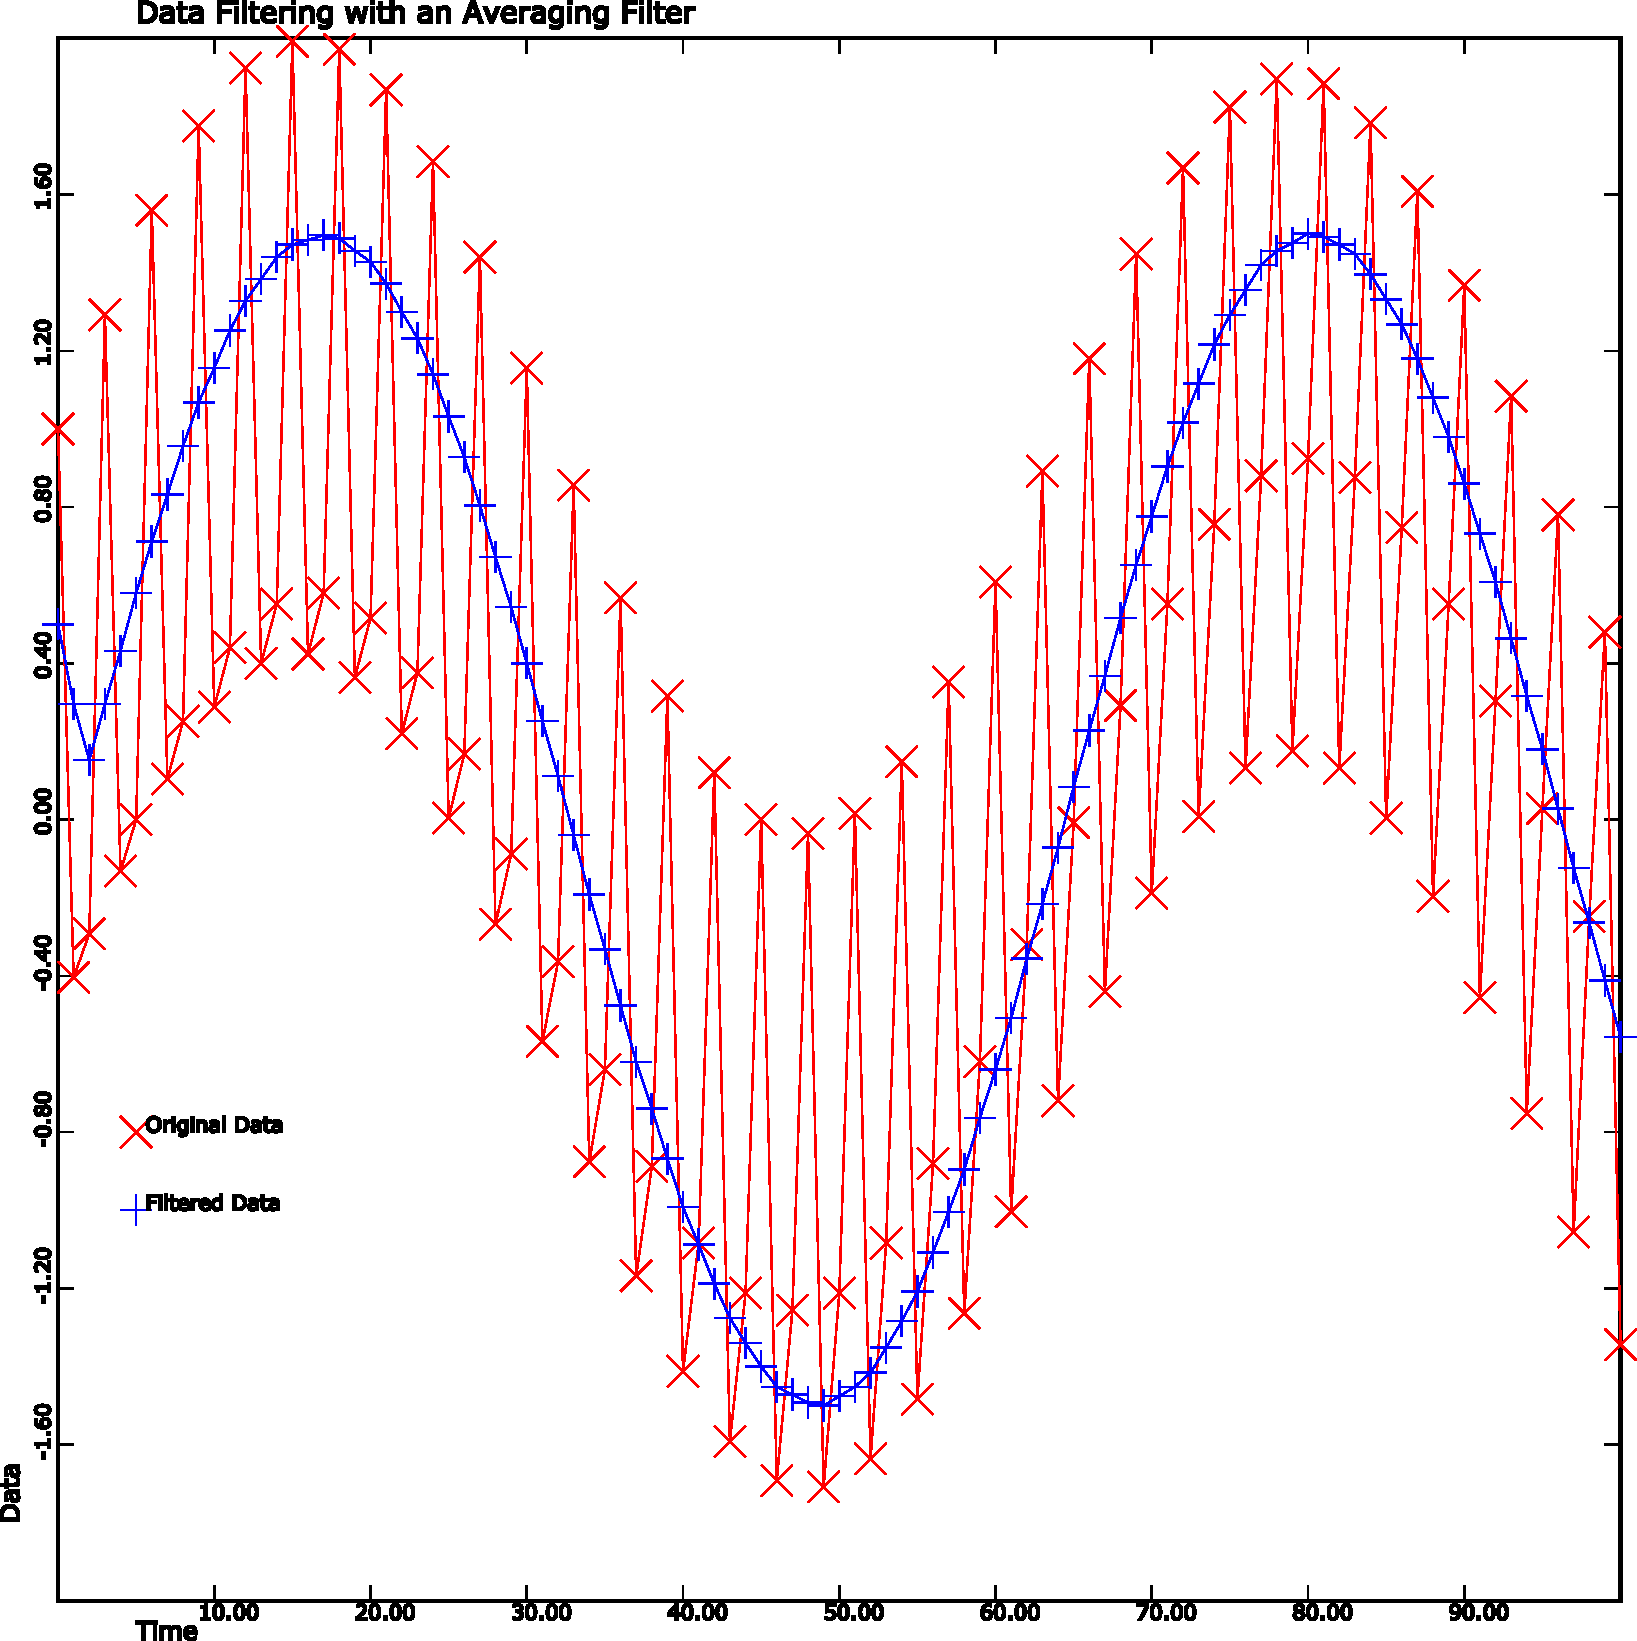
\includegraphics[scale=0.6]{filter-plot.pdf}
  \caption{Example Averaging Filter}
  \label{svg:Ave}
\end{figure}
\end{lstlisting}

Some example figures are shown in Figures \ref{svg:Ave} and \ref{svg:Prob}.

\begin{figure}
  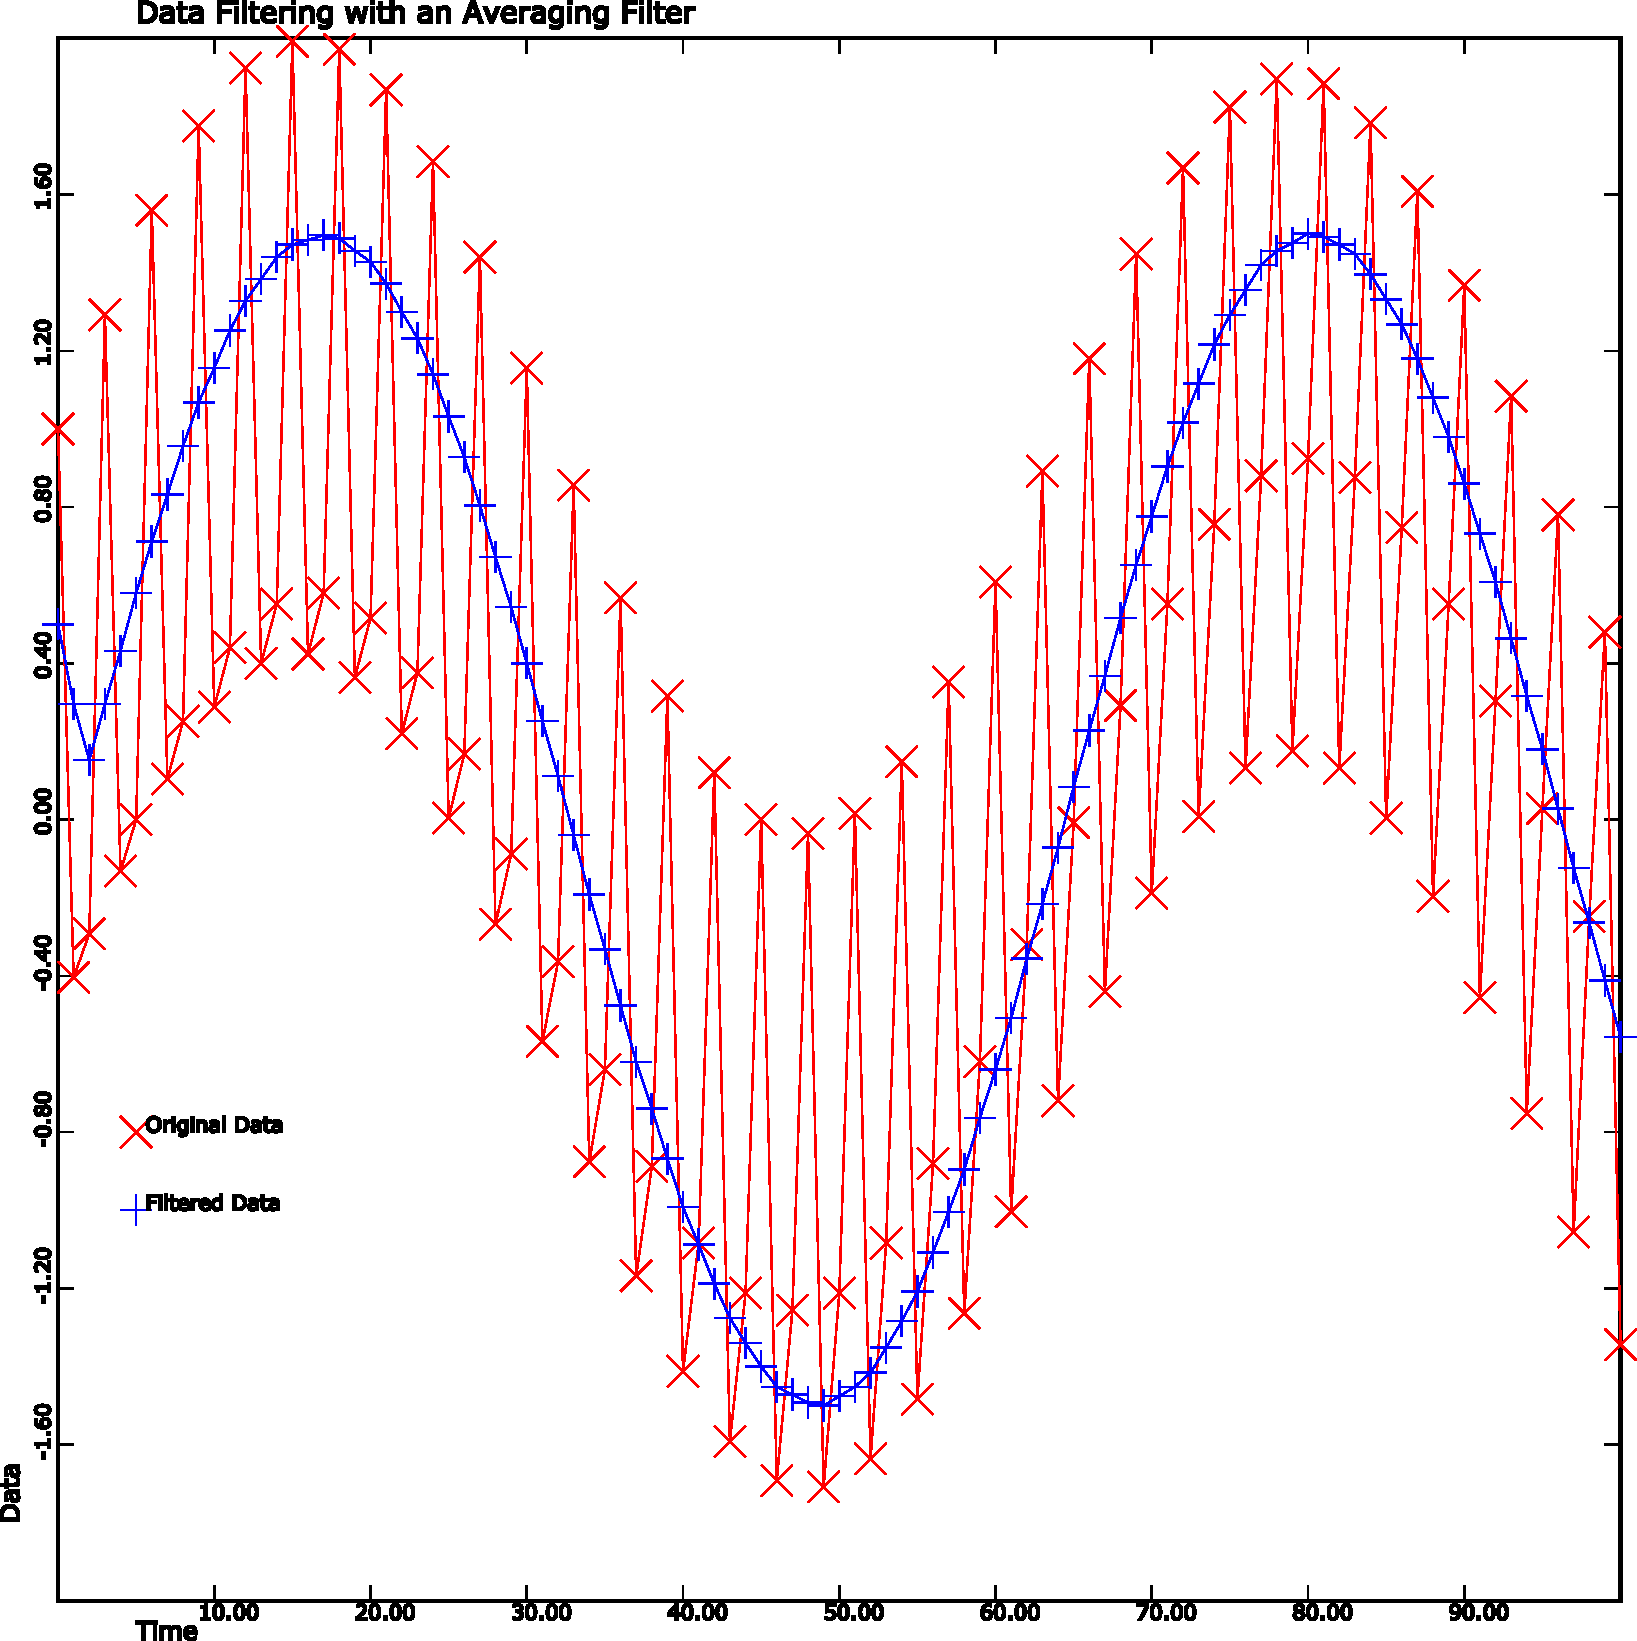
\includegraphics[scale=0.6]{filter-plot.pdf}
  \caption{Example Averaging Filter}
  \label{svg:Ave}
\end{figure}

\begin{figure}
  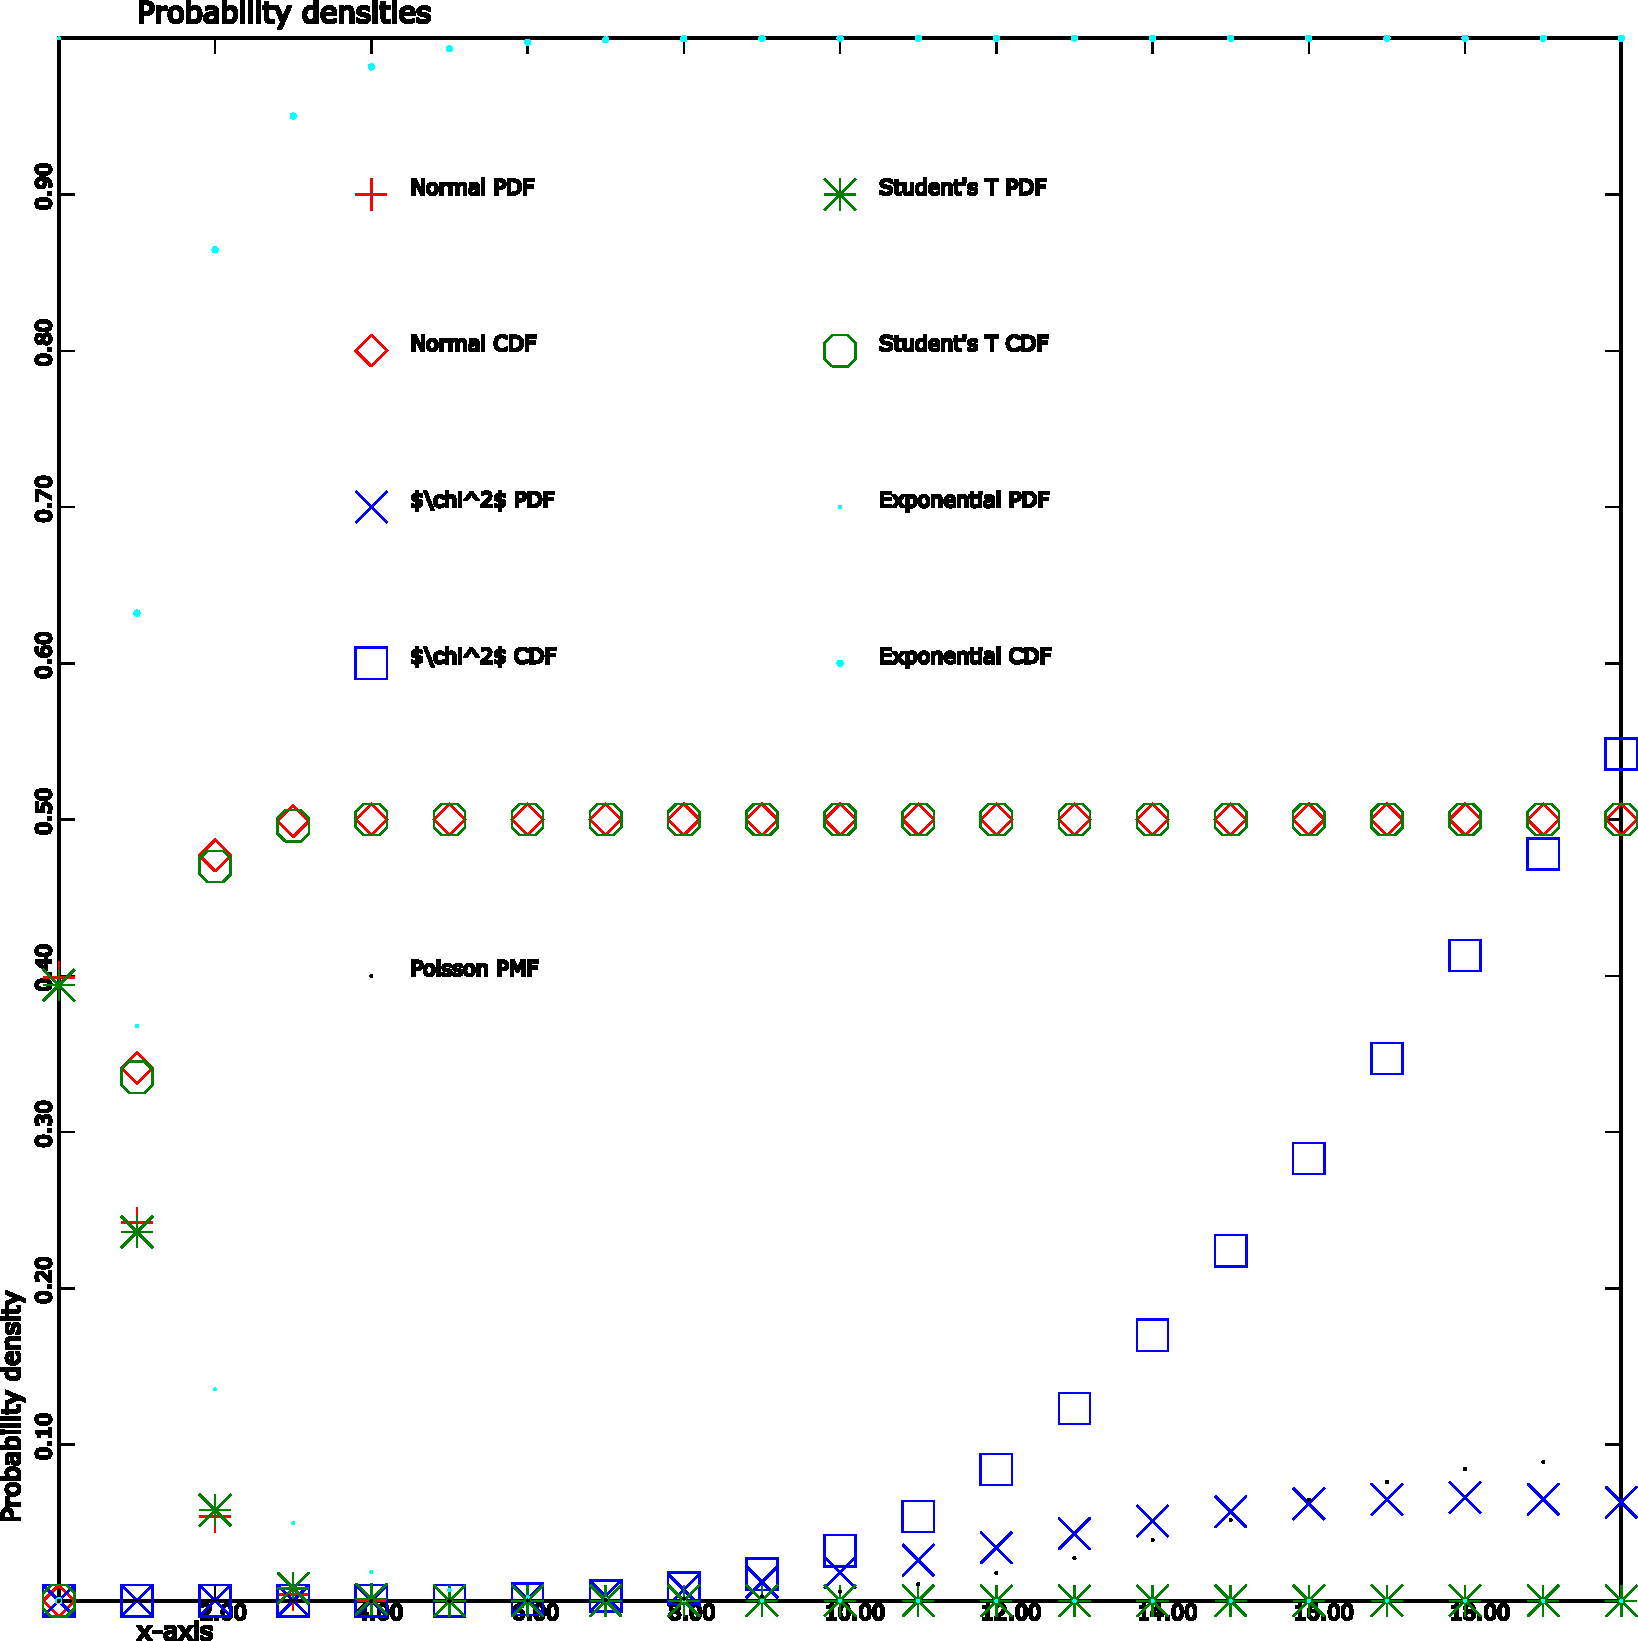
\includegraphics[scale=0.6]{stat-plot.pdf}
  \caption{Probability Density Functions}
  \label{svg:Prob}
\end{figure}

%--------------------------------------------------------------------------------------------------
\section{BBS.Numerical.polynomial\_complex}
This is a generic package with a complex package parameter, \datatype{cmplx}.  This parameter has datatypes \datatype{cmplx.Complex} and \datatype{cmplx.Real}.

The package defines the datatype \datatype{poly} as \datatype{array (Natural range  <>) of cmplx.Complex}, with a constraint that \datatype{poly'First} is equal to 0.  Polynomials are implemented as an array of coefficients where the index in the array represents the exponent of the independent variable.  The index range starts from 0 and extends to the order of the polynomial.  This package contains operations on polynomials with complex number coefficients and independent variable.

\subsection{Basic Operations}
The basic binary operations on polynomials, addition (`+'), subtraction (`-'), and multiplication (`*') are implemented and assigned to the operators.  Unary negation (`-') is implemented and assigned to the `-' operator.  Multiplication of a polynomial by a scalar is implemented and assigned to the `*' operator for both scalar first and scalar last.

Division is based on the \function{polydiv()} implementation of synthetic division in \cite{NR-C}.  It divides two polynomials and returns a remainder and quotient.
\begin{align*}
  \frac{u}{v} = q, r
\end{align*}
\begin{lstlisting}
procedure divide(u, v : poly; q : out poly; r : out poly)
      with pre => (q'Last >= (u'Last - v'Last)) and
                  (r'Last >= (v'Last - 1)) and
                  (u'Last >= v'Last);
\end{lstlisting}
\begin{itemize}
  \item $u$ - The numerator for division.
  \item $v$ - The denominator for division.
  \item $q$ - The quotient result of the division.
  \item $r$ - The remainder from the division.
  \item This is a procedure, thus nothing is returned.
\end{itemize}

\subsection{Other Operations}

Evaluate a polynomial at a specific value of the independent variable.
\begin{lstlisting}
function evaluate(p : poly; x : cmplx.Complex) return cmplx.Complex;
\end{lstlisting}
\begin{itemize}
  \item $p$ - The polynomial to evaluate.
  \item $x$ - The independent variable.
  \item Returns the value of the polynomial evaluated at $x$.
\end{itemize}

Eliminate any leading coefficients with a zero value.  For example $0x^3+x^2+3x+4$ gets trimmed to $x^2+3x+4$.
\begin{lstlisting}
function trim(p : poly) return poly
      with post => (trim'Result'Last <= p'Last);
\end{lstlisting}
\begin{itemize}
  \item $p$ - The polynomial to trim.
  \item Returns the trimmed polynomial of order equal to or less than the original polynomial.
\end{itemize}

Determine the order of a polynomial.  That is the maximum index with a non-zero value.
\begin{lstlisting}
function order(p : poly) return Natural;
\end{lstlisting}
\begin{itemize}
  \item $p$ - The polynomial to determine the order of.
  \item Returns the order of the polynomial.
\end{itemize}

\subsection{Utility}
For development or debugging purposes a simple print polynomial procedure is provided.

\begin{lstlisting}
procedure print(p : poly; fore, aft, exp : Natural);
\end{lstlisting}
\begin{itemize}
  \item $p$ - The polynomial to print.
  \item fore, aft, and exp - values passed in for floating point formatting.
  \item This is a procedure so no value is returned.  A representation of the polynomial is displayed on the default output.
\end{itemize}

\subsection{Calculus}
Integrals and derivatives of polynomials are fairly easy to generate.  So, functions are provided to take a polynomial and return the integral or the derivative.
\begin{align*}
  \int ax^n dx = a\frac{x^{n+1}}{n+1}+C
\end{align*}
The resulting polynomial for integration has order one greater than the original polynomial.
\begin{lstlisting}
function integrate(p : poly; c : cmplx.Complex) return poly
      with post => (integrate'Result'Last = (p'Last + 1));
\end{lstlisting}
\function{integrate(p : poly; c : cmplx.Complex) return poly}
\begin{itemize}
  \item $p$ - The polynomial to integrate.
  \item $c$ - The constant term.
  \item Returns the integral of $p$.
\end{itemize}

\begin{align*}
  \frac{d}{dx}x^n = n x^{n-1}
\end{align*}
The resulting polynomial for differentiation has order one less than the original polynomial.
\begin{lstlisting}
function derivative(p : poly) return poly
      with post => (((derivative'Result'Last = (p'Last - 1)) and (p'Last > 0)) or
                    ((derivative'Result'Last = 0) and (p'Last = 0)));
\end{lstlisting}
\begin{itemize}
  \item $p$ - The polynomial to differentiate.
  \item Returns the derivative of the original polynomial.
\end{itemize}

%--------------------------------------------------------------------------------------------------
\section{BBS.Numerical.polynomial\_real}
This is a generic package with a real type parameter, \datatype{F}.

The package defines the datatype \datatype{poly} as \datatype{array (Natural range  <>) of f'Base}, with a constraint that \datatype{poly'First} is equal to 0.  Polynomials are implemented as an array of coefficients where the index in the array represents the exponent of the independent variable.  The index range starts from 0 and extends to the order of the polynomial.  This package contains operations on polynomials with real number coefficients and independent variable.

\subsection{Basic Operations}
The basic binary operations on polynomials, addition (`+'), subtraction (`-'), and multiplication (`*') are implemented and assigned to the operators.  Unary negation (`-') is implemented and assigned to the `-' operator.  Multiplication of a polynomial by a scalar is implemented and assigned to the `*' operator for both scalar first and scalar last.

Division is based on the \function{poludiv()} implementation of synthetic division in \cite{NR-C}.  It divides two polynomials and returns a remainder and quotient.
\begin{align*}
  \frac{u}{v} = q, r
\end{align*}
\begin{lstlisting}
procedure divide(u, v : poly; q : out poly; r : out poly)
      with pre => (q'Last >= (u'Last - v'Last)) and
                  (r'Last >= (v'Last - 1)) and
                  (u'Last >= v'Last);
\end{lstlisting}
\begin{itemize}
  \item $u$ - The numerator for division.
  \item $v$ - The denominator for division.
  \item $q$ - The quotient result of the division.
  \item $r$ - The remainder from the division.
  \item This is a procedure, thus nothing is returned.
\end{itemize}

\subsection{Other Operations}

Evaluate a polynomial at a specific value of the independent variable.
\begin{lstlisting}
function evaluate(p : poly; x : f'Base) return f'Base;
\end{lstlisting}
\begin{itemize}
  \item $p$ - The polynomial to evaluate.
  \item $x$ - The independent variable.
  \item Returns the value of the polynomial evaluated at $x$.
\end{itemize}

Eliminate any leading coefficients with a zero value.  For example $0x^3+x^2+3x+4$ gets trimmed to $x^2+3x+4$.
\begin{lstlisting}
function trim(p : poly) return poly
      with post => (trim'Result'Last <= p'Last);
\end{lstlisting}
\begin{itemize}
  \item $p$ - The polynomial to trim.
  \item Returns the trimmed polynomial of order equal to or less than the original polynomial.
\end{itemize}

Determine the order of a polynomial.  That is the maximum index with a non-zero value.
\begin{lstlisting}
function order(p : poly) return Natural;
\end{lstlisting}
\begin{itemize}
  \item $p$ - The polynomial to determine the order of.
  \item Returns the order of the polynomial.
\end{itemize}

\subsection{Utility}
For development or debugging purposes a simple print polynomial procedure is provided.
\begin{lstlisting}
procedure print(p : poly; fore, aft, exp : Natural);
\end{lstlisting}
\begin{itemize}
  \item $p$ - The polynomial to print.
  \item fore, aft, and exp - values passed in for floating point formatting.
  \item This is a procedure so no value is returned.  A representation of the polynomial is displayed on the default output.
\end{itemize}

\subsection{Calculus}
Integrals and derivatives of polynomials are fairly easy to generate.  So, functions are provided to take a polynomial and return the integral or the derivative.
\begin{align*}
  \int ax^n dx = a\frac{x^{n+1}}{n+1}+C
\end{align*}
The resulting polynomial for integration has order one greater than the original polynomial.
\begin{lstlisting}
function integrate(p : poly; c : f'Base) return poly
      with post => (integrate'Result'Last = (p'Last + 1));
\end{lstlisting}
\begin{itemize}
  \item $p$ - The polynomial to integrate.
  \item $c$ - The constant term.
  \item Returns the integral of $p$.
\end{itemize}

\begin{align*}
  \frac{d}{dx}x^n = n x^{n-1}
\end{align*}
The resulting polynomial for differentiation has order one less than the original polynomial.
\begin{lstlisting}
function derivative(p : poly) return poly
      with post => (((derivative'Result'Last = (p'Last - 1)) and (p'Last > 0)) or
                    ((derivative'Result'Last = 0) and (p'Last = 0)));
\end{lstlisting}
\begin{itemize}
  \item $p$ - The polynomial to differentiate.
  \item Returns the derivative of the original polynomial.
\end{itemize}

%--------------------------------------------------------------------------------------------------
\section{BBS.Numerical.quaternion}
This is a generic package with a real type parameter, \datatype{F}.

Quaternions are an extension of complex numbers into three dimensions.  A quaternion $q$ is defined as follows:
\begin{align*}
  q=a+b\uvec{i}+c\uvec{j}+d\uvec{k}
\end{align*}
Where
\begin{align*}
  \uvec{i}^2+\uvec{j}^2+\uvec{k}^2=\uvec{i}\uvec{j}\uvec{k}=-1
\end{align*}

This package defines the datatype \datatype{quaternion} as a tagged record with fields $r$, $i$, $j$, and $k$, each of type \datatype{F'Base}.  This means that it is treated as an object and some of the functions can be called in object oriented fashion.

\subsection{Basic Operations}
The basic binary operations on polynomials, addition (`+'), subtraction (`-'), multiplication (`*'), and division (`/') are implemented and assigned to the operators.  Multiplication of a polynomial by a scalar is implemented and assigned to the `*' operator for both scalar first and scalar last.  Note that with quaternions, multiplication is not necessarily commutative.  That is, in general $q_1 q_2 \neq q_2 q_1$.

\subsection{Other Operations}

Compute the magnitude of a quaternion (similar to absolute value) using $|q| = \sqrt{a^2+b^2+c^2+d^2}$.  Note that overflow is possible if any of $a$, $b$, $c$, $d$ are greater than the square root of the maximum value of \datatype{F'Base}.
\begin{lstlisting}
function magnitude(self : in quaternion) return f'Base;
\end{lstlisting}
\begin{itemize}
  \item $self$ - The quaternion to have its magnitude returned.
  \item Returns the magnitude of $self$.
\end{itemize}

Scale a quaternion to have a magnitude of 1 (a unit vector).  Since the magnitude is computed to be used as a scale factor, the same comments about overflow apply here.
\begin{lstlisting}
function normalize(self : in quaternion) return quaternion;
\end{lstlisting}
\begin{itemize}
  \item $self$ - The quaternion to be scaled.
  \item Returns a unit quaternion with the same direction as $self$.
\end{itemize}

%--------------------------------------------------------------------------------------------------
\section{BBS.Numerical.random}
This is not a generic package.

The Ada standard doesn't specify the random number generator to be used.  This package provides two different methods of generating a sequence of pseudo-random numbers.  This package defines an abstract tagged type, \datatype{RNG}, which is used to specify the operations that all random number generators need to provide.  It also defines the type \datatype{double} as \datatype{digits 12}.  This type is used to convert the \datatype{uint32} output of the random number generator into a real number in the range 0.0 to 1.0.

I wrote implementations of these in Java around 2010.  The following routines are based on the Java routines translated into Ada.

\subsection{Linear Congruent Generator}
The linear congruent generator is based on algorithms in \cite{NR-C}.  It provides a datatype \datatype{LCG} which defines an object containing the parameters and state for the generator.  This allows for multiple random number streams with the same or different parameters.

The linear congruent generator is based on the formula:
\begin{align*}
  R_{n+1} = (aR_n + c) \mod modulus
\end{align*}
where $R_0$ is the starting point or seed of the generator.  This generator is fairly fast and has minimal state information.  With a proper choice of parameters, it can produce decent results.  With an improper choice of parameters, the results are not very random.

Initialize the \datatype{LCG} object to some default values.
\begin{lstlisting}
overriding
procedure init(self : in out LCG);
\end{lstlisting}
\begin{itemize}
  \item $self$ - The LCG object to initialize.
\end{itemize}

Initialize the \datatype{LCG} object with specified parameters.  Since the linear-congruent generator is commonly used, parameters can be chosen to emulate the sequence from many other systems.
\begin{lstlisting}
procedure init(self : in out LCG; seed, modulus, a, c : uint32);
\end{lstlisting}
\begin{itemize}
  \item $self$ - The LCG object to initialize.
  \item $seed$ - The initial value for the generator.
  \item $modulus$ - The modulus for the generator.
  \item $a$ - The $a$ coefficient in the generator formula.
  \item $c$ - The $c$ coefficient in the generator formula.
\end{itemize}

The initial, ($seed$) value can be set in a generator without changing the other values.
\begin{lstlisting}
procedure setSeed(self : in out LCG; seed : uint32);
\end{lstlisting}
\begin{itemize}
  \item $self$ - The LCG object to adjust.
  \item $seed$ - The new seed value.
\end{itemize}

Return the next random number in raw format as a \datatype{uint32}.
\begin{lstlisting}
overriding
function getNext(self : in out LCG) return uint32;
\end{lstlisting}
\begin{itemize}
  \item $self$ - The LCG object to get the next random number from.
  \item Returns the next \datatype{uint32} in the sequence.
\end{itemize}

Return the next random number as a floating point in the range 0.0 to 1.0.  This can then be cast to the desired real number type.
\begin{lstlisting}
overriding
function getNextF(self : in out LCG) return double;
\end{lstlisting}
\begin{itemize}
  \item $self$ - The LCG object to get the next random number from.
  \item Returns the next real number in the sequence.
\end{itemize}

\subsection{Mersenne Twister Generator}
The mersenne twister generator is based on algorithms in \cite{MT19937}.  It provides a datatype \datatype{MT} which defines an object containing the parameters and state for the generator.  This allows for multiple random number streams with the same or different parameters.  While this generator is fairly fast, it requires about 624 \datatype{uint32} values of state information, thus considerably more memory than \datatype{LCG}.

Initialize the \datatype{MT} object to some default values.
\begin{lstlisting}
overriding
procedure init(self : in out MT);
\end{lstlisting}
\begin{itemize}
  \item $self$ - The MT object to initialize.
\end{itemize}

Initialize the \datatype{MT} object with specified seed.
\begin{lstlisting}
procedure init(self : in out MT; seed : uint32);
\end{lstlisting}
\begin{itemize}
  \item $self$ - The LCG object to initialize.
  \item $seed$ - The initial value for the generator.
\end{itemize}

Return the next random number in raw format as a \datatype{uint32}.
\begin{lstlisting}
overriding
function getNext(self : in out MT) return uint32;
\end{lstlisting}
\begin{itemize}
  \item $self$ - The MT object to get the next random number from.
  \item Returns the next \datatype{uint32} in the sequence.
\end{itemize}

Return the next random number as a floating point in the range 0.0 to 1.0.  This can then be cast to the desired real number type.
\begin{lstlisting}
overriding
function getNextF(self : in out MT) return double;
\end{lstlisting}
\begin{itemize}
  \item $self$ - The MT object to get the next random number from.
  \item Returns the next real number in the sequence.
\end{itemize}

%--------------------------------------------------------------------------------------------------
\section{BBS.Numerical.regression}
This is a generic package with a real type parameter, \datatype{F}.  It defines the following datatypes:
\begin{itemize}
  \item \datatype{point} which is a record of two fields: $x$ and $y$, both of which are \datatype{F'Base}.
  \item \datatype{data\_array} as an array of \datatype{point}.
  \item \datatype{simple\_linreg\_result} is a record containing the results of simple linear regression.  The fields are:
  \begin{itemize}
    \item $a$ - The Y intercept
    \item $b$ - The slope
    \item $SSe$ - The sum of square errors
    \item $var$ - The sum of square errors normalized by the degrees of freedom ($n-2$).
    \item $Bvar$ - The variance of the slope.
    \item $cor$ - The correlation coefficient (R) (note that correlation does not imply causation).
  \end{itemize}
\end{itemize}

\subsection{Simple Linear Regression}
Given a set of ($x$, $y$) points where $x$ is assumed to have no error, and the errors on $y$ are assumed to have a mean of zero, normal distribution, and constant variance, find the line, $y=ax+b+\epsilon$, where $\epsilon$ is the error, that best fits the data.
\begin{lstlisting}
function simple_linear(d : data_array) return simple_linreg_result;
\end{lstlisting}
\begin{itemize}
  \item $d$ - An array of the data points to analyze.
  \item Returns a record of type \datatype{simple\_linreg\_result} containing the parameters for the line as well as estimates of how good the fit is.
\end{itemize}

%--------------------------------------------------------------------------------------------------
\section{BBS.Numerical.roots\_complex}
This is a generic package with a complex package parameter, \datatype{cmplx}.  This has datatypes \datatype{cmplx.Complex} and \datatype{cmplx.Real}.  It contains methods for finding roots of equations with complex variables.

It defines the following datatypes:
\begin{itemize}
   \item \datatype{test\_func} as \datatype{access function (x : cmplx.complex) return cmplx.complex}
   \item \datatype{errors} as an enumeration of \datatype{(none, bad\_args, no\_solution)}
\end{itemize}

Solve for (possibly) complex roots using Mueller's method.  Mueller's method starts with three initial approximations to the root and solves the parabola through these three points to produce the next approximation.
\begin{lstlisting}
function mueller(test : test_func; x0, x2 : in out cmplx.complex;
         limit : in out Positive; err : out errors) return cmplx.complex;
\end{lstlisting}
\begin{itemize}
  \item $test$ - The function to find a root of.
  \item $x0$ and $x2$ - Starting points for the root finding
  \item $limit$ - The number of iterations.
  \item $err$ - An error code.
  \item Returns an estimate of a root of the function.
\end{itemize}

%--------------------------------------------------------------------------------------------------
\section{BBS.Numerical.roots\_real}
This is a generic package with a real type parameter, \datatype{F}.  It contains methods for finding roots of equations with complex variables.

It defines the following datatypes:
\begin{itemize}
   \item \datatype{test\_func} as \datatype{access function (x : f'Base) return f'Base}
   \item \datatype{errors} as an enumeration of \datatype{(none, bad\_args, no\_solution)}
\end{itemize}

\subsection{Linear Methods}
If there is an odd number of roots between the lower and upper limits, the bisection algorithm will always converge.  Each iteration simply halves the interval between the limits, keeping a root between them.  The result is the midpoint of the final interval after the specified number of iterations.

The lower and upper values are updated during the iterations to provide an interval containing the root.
\begin{lstlisting}
function bisection(test : test_func; lower, upper : in out f'Base;
         limit : Positive; err : out errors) return f'Base;
\end{lstlisting}
\begin{itemize}
  \item $test$ - The function to find a root of.
  \item $lower$ - The lower bound of the interval for the root.
  \item $upper$ - The upper bound of the interval for the root.
  \item $limit$ - The number of iterations.
  \item $err$ - An error code.
  \item Returns an estimate of a root of the function.
\end{itemize}

If there is an odd number of roots between the lower and upper limits, the secant method will always converge.  Each stage of the iteration identifies a point where a line between the lower and upper values crosses the axis.  This point is used instead of the midpoint in the bisection algorithm.

Depending on the function, this can converge to a root much faster than the bisection algorithm.  On the other had, it can also converge much slower.

The lower and upper values are updated during the iterations to provide an interval containing the root.  If the root is exact, the lower and upper values are equal to the returned value.

This method will fail if during the process, the function values at the upper and lower bounds are ever equal.  This will cause a divide by zero error.
\begin{lstlisting}
function seacant(test : test_func; lower, upper : in out f'Base;
         limit : Positive; err : out errors) return f'Base;
\end{lstlisting}
\begin{itemize}
  \item $test$ - The function to find a root of.
  \item $lower$ - The lower bound of the interval for the root.
  \item $upper$ - The upper bound of the interval for the root.
  \item $limit$ - The number of iterations.
  \item $err$ - An error code.
  \item Returns an estimate of a root of the function.
\end{itemize}

\subsection{Mueller's Method}
Mueller's method uses three points to model a quadratic curve and uses that to find a candidate root.    Unlike the bisection method, Mueller's method does not require a root to be located within the three points.  This can potentially be used to find complex roots, however this implementation does not.

This method will fail if the function value at the three points is equal.

In this implementation, the user provides two points and the third is generated as the average of these two points.  This keeps the call the same as the bisection and secant functions.

Note that for this algorithm, the x0 and x2 values are not necessarily meaningful as upper and lower bounds for the root, except that they are both set equal to the return value if the root is exact.

Note that the success may be sensitive to the choice of x0 and x2.  If you know that a root exists and get a no\_solution error, try different values.
\begin{lstlisting}
function mueller(test : test_func; x0, x2 : in out f'Base;
         limit : in out Positive; err : out errors) return f'Base;
\end{lstlisting}
\begin{itemize}
  \item $test$ - The function to find a root of.
  \item $x0$ and $x2$ - Starting points for the root finding
  \item $limit$ - The number of iterations.
  \item $err$ - An error code.
  \item Returns an estimate of a root of the function.
\end{itemize}

%--------------------------------------------------------------------------------------------------
\section{BBS.Numerical.statistics}
This is a generic package with a real type parameter, \datatype{F}.  It contains a number of statistics related routines.  It defines the datatype \datatype{data\_array} as \datatype{array (Integer range <>) of F'Base}.

\subsection{Data Statistics}
These routines compute statistics on the values in a \datatype{data\_array}.

Compute the mean of a set of values.  For $n$ values, computes:
\begin{align*}
  m = \frac{1}{n}\sum_{i=1}^n d_i
\end{align*}
\begin{lstlisting}
function mean(d : data_array) return F'Base;
\end{lstlisting}
\begin{itemize}
  \item $d$ - The array containing the data.
  \item Returns the mean value of the data.
\end{itemize}

Compute the limits of a set of data.
\begin{lstlisting}
procedure limits(d : data_array; min : out F'Base; max : out F'Base);
\end{lstlisting}
\begin{itemize}
  \item $d$ - The array containing the data.
  \item $min$ - Output as the minimum value in the array.
  \item $max$ - Output as the maximum value in the array.
  \item This is a procedure and does not return a value.
\end{itemize}

Compute the variance of a set of data.  Since computing the variance also requires computing the mean, this procedure returns both values.
\begin{lstlisting}
procedure variance(d : data_array; var : out F'Base; mean : out F'Base);
\end{lstlisting}
\begin{itemize}
  \item $d$ - The array containing the data.
  \item $var$ - Output as the variance of the data in the array.
  \item $mean$ - Output as the mean of the data in the array.
  \item This is a procedure and does not return a value.
\end{itemize}

\subsection{Probability Distributions}
Note on naming conventions for probability distributions.  For continuous distribution functions, there are generally two functions.  The one with the ``\_pdf'' suffix is the probability density function.  The one with the ``\_cdf'' suffix is the cumulative distribution function.  For discrete functions, the ``\_pmf'' suffix is for the probability mass function.

\subsubsection{Normal Distribution}
Compute the standard normal distribution where the PDF is given by $x = e^{-p^2}$.
\begin{lstlisting}
function normal_pdf(p : F'Base) return F'Base;
\end{lstlisting}
\begin{itemize}
  \item $p$ - The value.
  \item Returns the probability density at point $p$.
\end{itemize}

Compute the normal distribution with a specified mean and standard deviation ($\sigma$).
\begin{lstlisting}
function normal_pdf(p, mean, sigma : F'Base) return F'Base;
\end{lstlisting}
\begin{itemize}
  \item $p$ - The value.
  \item $mean$ - The mean of the distribution.
  \item $sigma$ - The standard deviation of the distribution.
  \item Returns the probability density at point $p$.
\end{itemize}

Compute the normal cumulative distribution for the standard normal function.  This is computed by integrating the standard normal function from $a$ to $b$.
\begin{align*}
  p = \int^b_a e^{-x^2} dx
\end{align*}
\begin{lstlisting}
function normal_cdf(a, b : F'Base; steps : Positive) return F'Base;
\end{lstlisting}
\begin{itemize}
  \item $a$ - Starting point for integration.
  \item $b$ - Ending point for integration.
  \item $steps$ - Number of steps for Simpson's rule integration.
  \item Returns the cumulative probability between $a$ and $b$.
\end{itemize}

\subsubsection{$\chi^2$ Distribution}
Compute the $\chi^2$ distribution where the PDF is given by:
\begin{align*}
  p = \frac{1}{2^{\frac{k}{2}}\Gamma(\frac{k}{2})}x^{\frac{k}{2}-1}e^{-\frac{x}{2}}
\end{align*}
\begin{lstlisting}
function chi2_pdf(x : f'Base; k : Positive) return f'Base;
\end{lstlisting}
\begin{itemize}
  \item $x$ - The value.
  \item $k$ - The number of degrees of freedom.  Must be greater than zero.
  \item Returns the probability density at point $x$.
\end{itemize}

Compute the cumulative $\chi^2$ between $a$ and $b$.
\begin{lstlisting}
function chi2_cdf(a, b : F'Base; k, steps : Positive) return F'Base;
\end{lstlisting}
\begin{itemize}
  \item $a$ - Starting point for integration.
  \item $b$ - Ending point for integration.
  \item $steps$ - Recursion depth for adaptive Simpson's rule integration.
  \item Returns the cumulative probability between $a$ and $b$.
\end{itemize}

\subsubsection{Student's T Distribution}
Compute the student's t distribution where the PDF is given by:
\begin{align*}
  p = \frac{\Gamma(\frac{\nu+1}{2})}{\sqrt{\pi\nu}\Gamma(\frac{\nu}{2})}(1+\frac{t^2}{\nu})^{-\frac{\nu+1}{2}}
\end{align*}
\begin{lstlisting}
function studentT_pdf(t : f'Base; nu : Positive) return f'Base;
\end{lstlisting}
\begin{itemize}
  \item $t$ - The value.
  \item $nu$ - Shape parameter ($\nu$).
  \item Returns the probability density at point $t$.
\end{itemize}

Compute the cumulative student t between $a$ and $b$.
\begin{lstlisting}
function studentT_cdf(a, b : F'Base; nu, steps : Positive) return F'Base;
\end{lstlisting}
\begin{itemize}
  \item $a$ - Starting point for integration.
  \item $b$ - Ending point for integration.
  \item $steps$ - Recursion depth for adaptive Simpson's rule integration.
  \item Returns the cumulative probability between $a$ and $b$.
\end{itemize}

\subsubsection{Exponential Distribution}
Compute the exponential distribution where the PDF is given by $\lambda e^{-\lambda x}$.
\begin{lstlisting}
function exp_pdf(x, lambda : f'Base) return f'Base;
\end{lstlisting}
\begin{itemize}
  \item $x$ - The value.
  \item $lambda$ - The shape parameter ($\lambda$)
  \item Returns the probability at point $x$.
\end{itemize}

Compute the cumulative exponential between $0$ and $x$.  This is given by $1-e^{-\lambda x}$
\begin{lstlisting}
function exp_cdf(x, lambda : f'Base) return f'Base;
\end{lstlisting}
\begin{itemize}
  \item $x$ - The value.
  \item $lambda$ - The shape parameter ($\lambda$)
  \item Returns the cumulative probability from $0$ to $x$.
\end{itemize}

\subsubsection{Poisson Distribution}
Since the Poisson Distribution is a discrete distribution rather than a cumulative distribution, we compute a probability mass function.  This is given by:
\begin{align*}
  p(k) = \frac{\lambda^k e^{-\lambda}}{k!}
\end{align*}
\begin{lstlisting}
function poisson_pmf(k : Natural; lambda : Positive) return f'Base;
\end{lstlisting}
\begin{itemize}
  \item $k$ - The value.
  \item $lambda$ - The shape parameter ($\lambda$)
  \item Returns the probability of $k$.
\end{itemize}

\subsection{Statistical Tests}
\subsubsection{Student's T Tests}
Use the one sample t test to compare the mean of a sample to a specified mean.  Given the sample mean, $\bar{x}$, the sample standard deviation, $s$, and the sample size, $n$, compute the student's t statistic for the difference between $\bar{x}$ and the specified mean, $\mu_0$.
\begin{lstlisting}
function studentT_one(x_bar, mu0, s, n : f'Base) return f'Base;
\end{lstlisting}
\begin{itemize}
  \item $x_bar$ - The sample mean ($\bar{x}$).
  \item $mu0$ - The specified mean ($\mu_0$).
  \item $s$ - The sample standard deviation ($s$).
  \item $n$ - The number of samples ($n$).
  \item Returns the t statistic for the difference between the $\bar{x}$ and $\mu_0$.
\end{itemize}

%--------------------------------------------------------------------------------------------------
\section{BBS.Numerical.vector}
This is a generic package with a real type parameter, \datatype{F}.  It contains some vector related routines.  It defines the datatype \datatype{vect} as \datatype{array (integer range <>) of f'Base}

\subsection{Basic Operations}
Addition (`+') and subtraction (`-') of vectors is defined and assigned to the operators.  These operations require both vectors to have the same index ranges and return a vector with the same index range.

Multiplication (`*') of vectors is defined and assigned to the operator.  It requires both vectors to have the same index and returns the scaler dot product of the vectors.

Multiplication (`*') of a vector by a scaler is defined and assigned to the operator for both scaler first and scaler last.  It returns a vector with the same index range as the source vector.

\subsection{Other Operations}

Compute the magnitude of a vector by taking the square root of the sum of the squares of the elements.  Note that overflow is possible if any of the elements are greater than the square root of the maximum value of \datatype{F'Base}.
\begin{lstlisting}
function magnitude(self : in vect) return f'Base;
\end{lstlisting}
\begin{itemize}
  \item $self$ - The vector to take the magnitude of.
  \item Returns the magnitude of the vector.
\end{itemize}

Scale the elements in a vector so that the vector has a magnitude of one.  The same overflow warning for the \function{magnitude} function also apply here.
\begin{lstlisting}
function normalize(self : in vect) return vect;
\end{lstlisting}
\begin{itemize}
  \item $self$ - The vector to normalize.
  \item Returns the normalized vector.
\end{itemize}

%========================================================
\clearpage
\addcontentsline{toc}{chapter}{Bibliography}
\nocite{NA3rd}
\bibliographystyle{plain}
\bibliography{Numerical.bib}

\end{document}

